%%%%%%%%% Dokumentenklasse
\documentclass[
	%fontsize=12pt,% Times New Roman
	fontsize=11pt,% Andere
	paper=a4,
	]{scrartcl}


%%%%%%%%% HTW Anforderungen
\usepackage[
	margin=2.5cm,% Seitenränder auf 2,5cm setzen
%1	bottom=3.1cm,
%	showframe,% <- only to show the page layout
]{geometry}
%\usepackage{mathptmx}% Times New Roman
%\usepackage[scaled=0.92]{helvet}% quasi Arial
%\renewcommand{\familydefault}{\sfdefault}
%\usepackage{roboto}% Roboto Font


%%%%%%%%% Literatur
\usepackage[
	backend = biber,
	style=alphabetic,% Alphatischer Style [abc12]
	maxalphanames=3,% Kurzform besteht aus maximal den ersten Buchstaben der Nachnamen der ersten drei Autoren (wenn min. 3 gegeben)
	minalphanames=3,% Kurzform besteht aus minimal drei Buchstaben der Nachnamen der Autoren
	]{biblatex}% Nützliche Anleitung: http://www.nagel-net.de/Latex/DOKU/DTK-2_2008-biblatex-Teil1.pdf
\usepackage{notoccite}% don't show cites in toc, list of figures, etc.


%%%%%%%%% Code
\usepackage[
	newfloat,
%	outputdir=out,
%	cache=false,
	]{minted}% Code highlighting
\usepackage{caption}% Neue Environment um Code-Blöcken eine Caption zu geben
\newenvironment{code}{\captionsetup{type=listing}}{}
\SetupFloatingEnvironment{listing}{name=Quellcode}


%%%%%%%%% Sprachpackages
\usepackage[
	T1
	]{fontenc}% Textzeichen für westeuropäische Sprachen
\usepackage[
	utf8
	]{inputenc}% Umlaute
\usepackage[
	ngerman,% Deutsch
	english,% Englisch
	]{babel}% Automatisch erzeugte Texte werden auf Deutsch ausgegeben
\usepackage[
	ngerman
	]{datetime2}% Datumsformate
\usepackage{csquotes}% This package provides advanced facilities for inline and display quotations; should be loaded after minted
\usepackage{textcomp}% Einige Symbole
\usepackage[
	official
	]{eurosym}% €-Symbol


%%%%%%%%% Blind-Text
\usepackage{lipsum}
\usepackage{draftwatermark}

\SetWatermarkText{Draft: \today}
\SetWatermarkColor[gray]{0.5}
\SetWatermarkFontSize{1cm}
\SetWatermarkAngle{90}
\SetWatermarkHorCenter{20cm}


%%%%%%%%% Mathe & Naturwissenschaften
\usepackage[
%	fleqn
	]{amsmath}% Mathematische Formartierung
\usepackage{
	amssymb,% Mathematische Symbole
	amsfonts,% Mathematische Schriftarten
	}
\usepackage{siunitx}% Saubere Darestellung von SI Einheiten
\sisetup{
	locale = DE,% Deutsche Norm, Kommas werden z.B. erkannt
	per-mode=symbol,% Output a/b as \frac{a}{b} - in der Einheit
	quotient-mode=symbol,% Output a/b as \frac{a}{b} - im Quotienten
	fraction-function=\tfrac,
	range-phrase = {\text{~bis~}},
	sticky-per = true,% \per bleibt bestehen für mehr als eine Einheit
	separate-uncertainty,% Standardabweichung
}
\usepackage{mathtools}
\usepackage[
	version=4,
	]{mhchem}% chemische Gleichungen/Summenformeln


%%%%%%%%% Grafiken und Farben
\usepackage{graphicx}% viele grafische Befehle, z.B. \scalebox
\usepackage{
	xcolor,
	colortbl,
	}% Farben und Farbpaletten
\usepackage[
	export
	]{adjustbox}% Positionieren von Grafiken, left, right, center
\usepackage{float}% Floating Bilder, H-Befehl
\usepackage{mwe}% Für Abbildungsverzeichnis
\usepackage{graphics}% accommodate all needs for inclusion of graphics
\usepackage{subfigure}% support for the manipulation and reference of small or ‘sub’ figures and tables within a single figure or table environment
\usepackage{svg}% einbinden von svg Grafiken


%%%%%%%%% Diagramme
\usepackage{
	tikz,% Grafik-Paket
	stackengine,% versatile way to stack objects vertically in a variety of customizable ways
	}
\usepackage{pgfplots}% Plots
\pgfplotsset{compat=1.14}% Soll man wohl machen
\usetikzlibrary{patterns}% Patterns anstatt Farben


%%%%%%%%% Seitenformatierung
\makeatletter
\usepackage{microtype}% Verbesserte Formatierung; Sollte immer geladen werden
\g@addto@macro\@verbatim{\microtypesetup{activate=false}}
\makeatother
\usepackage[
	headsepline,% Vertikale Linie unterm Header
	plainheadsepline,
	automark,% Section im Header
	singlespacing=true,
	]{scrlayer-scrpage}% Paket zur Manipulation der Kopf- und Fußzeilen
\usepackage{adjustbox}% Elemente skalieren \scalebox
\usepackage{pdflscape}% ermöglicht einzelne Seiten im landscape mode darzustellen
\usepackage{abstract}% Abstract-Umgebung
\usepackage{setspace}% Spacing-Umgebung
\usepackage{verbatimbox}
\usepackage[htt]{hyphenat}% better linebreaks in long \texttt{•} etc.


%%%%%%%%% Tabellenumgebung
\usepackage{booktabs}% enhances the quality of tables
\usepackage{array}% extends the options for column formats
\usepackage{
	multirow,
	makecell
	}% mehrzeilige Tabellenzellen
\usepackage{tabu}% Moderneres tabularx


%%%%%%%%% Custom
\newenvironment{conditions}% New environment - Für saubere Darstellung gegebener Variablen
	{\par\vspace{\abovedisplayskip}\noindent\begin{tabular}{>{$}l<{$} @{${}={}$} l}}
	{\end{tabular}\par\vspace{\belowdisplayskip}}
\makeatletter% Roman Numbers in Text
\newcommand*{\rom}[1]{\expandafter\@slowromancap\romannumeral #1@}
\makeatother
\renewcommand*{\labelalphaothers}{\textsuperscript{+}}% superscript + instead of normal + in literature


%%%%%%%%% Querverweise
\usepackage[
	breaklinks,% URLs/DOIs vernünftig brechen
	]{hyperref}% Links im pdf % Muss das letzte Paket sein was lädt, außer glossaries
\hypersetup{
    colorlinks,
    linkcolor={red!40!black},
    citecolor={blue!50!black},
    urlcolor={blue!80!black}
}


% Kapitel, statt Abschnitt, Unterabschnitt, etc.
\addto\extrasngerman{
	\def
	\sectionautorefname{Kapitel}
}
\addto\extrasngerman{
	\def
	\subsectionautorefname{Kapitel}
}
\addto\extrasngerman{
	\def
	\subsubsectionautorefname{Kapitel}
}


%%%%%%%%% Abkürzungsverzeichnis:
\usepackage[% Paket für Glossaries und Acronym-Glossaries % Muss das letzte Paket sein was lädt
	acronym,
	automake,
	nopostdot,
	toc,
	nomain,
	shortcuts,
	nogroupskip,
	]{glossaries}


%%%%%%%%% Date Range

\renewcommand{\DTMdisplaydate}[6]{\DTMtwodigits{#1}.\DTMtwodigits{#2}.~{--}~\DTMtwodigits{#4}.\DTMtwodigits{#5}.}


%%%%%%%%% Sonstige Custom Befehle:
\def\Arbeit{\glqq Arbeit\grqq{}~}
\def\Arbeitdot{\glqq Arbeit\grqq}
\def\Ausbildung{\glqq Ausbildung\grqq{}~}
\def\dienst{\glqq dienstlich\grqq{}~}
\def\dienstdot{\glqq dienstlich\grqq}
\def\ego{\textit{eGo~100}~}
\def\egodot{\textit{eGo~100}}
\def\Eigenheim{\glqq Eigenheim\grqq{}~}
\def\Eigenheimdot{\glqq Eigenheim\grqq}
\def\Einkauf{\glqq Einkauf\grqq{}~}
\def\Einkaufdot{\glqq Einkauf\grqq}
\def\Erledigung{\glqq Erledigung\grqq{}~}
\def\Erledigungdot{\glqq Erledigung\grqq}
\def\Firmeparkplatz{\glqq Firmenparkplatz\grqq{}~}
\def\Firmeparkplatzdot{\glqq Firmenparkplatz\grqq}
\def\Firmeparkplaetzen{\glqq Firmenparkplätzen\grqq{}~}
\def\Firmeparkplaetzendot{\glqq Firmenparkplätzen\grqq{}}
\def\Freizeit{\glqq Freizeit\grqq{}~}
\def\Freizeitdot{\glqq Freizeit\grqq}
\def\Gewerbeparkplatz{\glqq Gewerbeparkplatz\grqq{}~}
\def\Gewerbeparkplatzdot{\glqq Gewerbeparkplatz\grqq}
\def\Kleinwagen{Szenarette \glqq Kleinwagen\grqq{}~}
\def\Kleinwagendot{Szenarette \glqq Kleinwagen\grqq}
\def\kmean{\textit{k-means-Clustering}~}
\def\kmeans{\textit{k-means-Clusterings}~}
\def\kmeansdot{\textit{k-means-Clusterings}}
\def\Lastgebiet{\glqq Lastgebiet\grqq{}~}
\def\Lastgebiete{\glqq Lastgebiete\grqq{}~}
\def\Lastgebietedot{\glqq Lastgebiete\grqq}
\def\Lastgebietes{\glqq Lastgebietes\grqq{}~}
\def\Lastgebieten{\glqq Lastgebieten\grqq{}~}
\def\nH{\glqq nach Hause\grqq{}~}
\def\nHdot{\glqq nach Hause\grqq}
\def\oeffen{\glqq Öffentlich\grqq{}~}
\def\oeffendot{\glqq Öffentlich\grqq}
\def\Plus{\texttt{+}}
\def\Straszenrand{\glqq Straßenrand\grqq{}~}
\def\Straszenranddot{\glqq Straßenrand\grqq}
\def\SzeFirmenparkplatz{Sensitivität \glqq Firmenparkplatz\grqq{}~}
\def\SzeFirmenparkplatzdot{Sensitivität \glqq Firmenparkplatz\grqq}
\def\UC{Lade~\textit{Use}~\textit{case}~}
\def\UCs{Lade~\textit{Use}~\textit{cases}~}
\def\Wohnanlage{\glqq Wohnanlage\grqq{}~}
\def\Wohnanlagedot{\glqq Wohnanlage\grqq}
\def\zH{\glqq zu Hause\grqq{}~}
\def\zHdot{\glqq zu Hause\grqq}% Packages

\addbibresource{02_lit.bib}% Literatur

% Abkürzungen
% s. documentation https://ctan.org/pkg/glossaries?lang=de
% \newacronym[
% shortplural = {}, -> Hier kann der Plural der Kurzform eigens eingestellt werden
% longplural = {}, -> Hier kann der Plural der ausgeschriebenen Form eigens eingestellt werden
% {html} -> label
% {HTML} -> short form
% {hypertext markup language} -> long form

\makeglossaries

%\setacronymstyle{long-short}
\newacronym[
	]{AC}{AC}{Alternating current}
\newacronym[
	]{BAU}{BAU}{Business as usual}
\newacronym[
    longplural={Biomasseanlagen},
	]{BMA}{BMA}{Biomasseanlage}
\newacronym[
	]{BEV}{BEV}{Battery electric vehicle}
\newacronym[
	]{DC}{DC}{Direct current}
\newacronym[
    longplural={dezentraler Erzeugungsanlagen},
	]{DEA}{DEA}{dezentrale Erzeugungsanlage}
\newacronym[
	longplural={Erneuerbaren-Energien-Gesetz},
	shortplural={EEG}
	]{EEG}{EEG}{Erneuerbare-Energien-Gesetz}
\newacronym[
    longplural={elektrischen Personenkraftwagen},
    shortplural={E-Pkw}
	]{EPKW}{E-Pkw}{elektrischer Personenkraftwagen}
\newacronym[
	]{EV}{EV}{Electric vehicle}
\newacronym[
	longplural={fluktuierenden erneuerbaren Energien}
	]{FEE}{fEE}{Fluktuierende erneuerbare Energien}
\newacronym[
	]{GHD}{GHD}{Gewerbe, Handel, Dienstleistungen}
\newacronym[
    shortplural={HS},
	]{HPC}{HPC}{High Power Charging}
\newacronym[
    shortplural={HS},
	]{HS}{HS}{Hochspannung}
\newacronym[
	longplural={Mobilität in Deutschland},
    shortplural={MiD 2017},
	]{MID}{MiD 2017}{Mobilität in Deutschland}
\newacronym[
	longplural={motorisiertem Individualverkehr},
    shortplural={MIV},
	]{MIV}{MIV}{motorisierter Individualverkehr}
\newacronym[
    shortplural={MS},
	]{MS}{MS}{Mittelspannung}
\newacronym[
	longplural={neuen europäischen Fahrzyklus},
    shortplural={NEFZ},
	]{NEFZ}{NEFZ}{Neuer Europäischer Fahrzyklus}
\newacronym[
    longplural={Netzgebietsklassen},
	]{NGK}{NGK}{Netzgebietsklasse}
\newacronym[
    shortplural={NS},
	]{NS}{NS}{Niederspannung}
\newacronym[
	]{PHEV}{PHEV}{Plug-in hybrid electric vehicle}
\newacronym[
    longplural={Personenkraftwagen},
    shortplural={Pkw}
	]{PKW}{Pkw}{Personenkraftwagen}
\newacronym[
    longplural={Photovoltaikanlagen},
	]{PVA}{PVA}{Photovoltaikanlage}
\newacronym[
    longplural={State of charge},
    shortplural={SOC}
	]{SOC}{SoC}{State of charge}
\newacronym[
    shortplural={V2G},
	]{V2G}{V2G}{Vehicle to grid}
\newacronym[
    longplural={Windenergieanlagen},
	]{WEA}{WEA}{Windenergieanlage}
\newacronym[
    longplural={Wärmepumpen},
    shortplural={WP},
	]{WP}{WP}{Wärmepumpe}% Abkürzungen

% Shortcuts for SI Values
% Grundlagen: https://www.namsu.de/Extra/pakete/Siunitx.html
% Gute Erklärung der Shortcuts: https://texwelt.de/fragen/2588/wie-schreibe-ich-zahlen-mit-einheiten-richtig

%\DeclareSIUnit{\BeladungsDichte}{\kilo\gram_{\textup{H\textup{2}}\per\kilo\gram_{\textup{FeTi}}}}		% Beladungsdichte
%\DeclareDocumentCommand\BeladungsDichte{O{}m}{\SI[#1]{#2}{\BeladungsDichte}}

%\DeclareSIUnit[]\NormVolumen
%{\text{\ensuremath{\cubic\meter_{\textup{i.N.}}}}}

%%%%%%% New SIValues

\DeclareSIUnit\sieuro{\mbox{\euro{}}}
\DeclareSIUnit\kw{\kilo\watt}
\DeclareSIUnit\mw{\mega\watt}
\DeclareSIUnit\gw{\giga\watt}
\DeclareSIUnit\kv{kV}
\DeclareSIUnit\kva{kVA}
\DeclareSIUnit\kwh{kWh}
\DeclareSIUnit\gwh{GWh}
\DeclareSIUnit\twh{TWh}
\DeclareSIUnit\kwhkm{\kwh\per100~\km}
\DeclareSIUnit\MioMen{\text{Millionen~Menschen}}
\DeclareSIUnit\MioStk{\text{Millionen~Stück}}
\DeclareSIUnit\MioStkSC{\text{Mio.~Stk.}}

%%%%%%% New complete Commands

\NewDocumentCommand\DeclareNewQuantity{mmm}{%
	\DeclareSIUnit{#2}{#3}%
	\DeclareDocumentCommand{#1}{O{}m}{\SI[##1]{##2}{#2}}%
}

\DeclareNewQuantity
	\Dichte
	\dichte
	{\kg\per\cubic\meter}% Custom SI-Einheiten

\begin{document}
\selectlanguage{ngerman}

\pagenumbering{Roman}% Roman Page Numbers
\pagenumbering{gobble}% gobble Page Numbers

\begin{titlepage}
    \begin{figure}
    \centering
    \begin{subfigure}{.5\textwidth}
      \hspace*{-1.5cm}
\includegraphics[height=2cm, center]{Bilder/S04_HTW_Berlin_Logo_pos_FARBIG_RGB}
    \end{subfigure}%
    \begin{subfigure}{.5\textwidth}
      \hspace*{1.5cm}
\includegraphics[height=2cm, center]{Bilder/RLI_logo_transparent}
    \end{subfigure}
    \end{figure}

	\vspace*{0.1cm}
    
	\centering
	\par\noindent\rule{\textwidth}{0.5pt}
	{\huge\bfseries Analyse des Einflusses\\
	netzdienlicher Ladestrategien auf Verteilnetze\\
	aufgrund der zunehmenden\\
	Netzintegration von Elektrofahrzeugen\par}
	\par\noindent\rule{\textwidth}{1pt}\par
	
	\vspace*{2cm}
	
	{\Large Kilian \textsc{Helfenbein}\par}
	{\large \textit{554994}\par}
	
	\vspace{1cm}
	
	{\scshape\huge Masterarbeit\par}
	
	\vspace{1cm}
	
	{\scshape\Large Hochschule für Technik und Wirtschaft Berlin \par}
	
	\vspace{1cm}
	
	Im Studiengang:\par
	{\scshape\large Regenerative Energien\par}
	
	\vspace{.5cm}
	
	Am Fachbereich:\par
	{\scshape\large Ingenieurwissenschaften {--} Energie und Information\par}
	
	\vfill
	
	{\large Berlin\\
	\today\par}
	
	\vfill
	
	% Bottom of the page
	{\large Betreuer$^*$in:\par
	Prof.~Dr.-Ing.~Jan Hanno \textsc{Carstens}\\
	Birgit \textsc{Schachler}}
\end{titlepage}% Titlepage

\pagenumbering{Roman}% Roman Page Numbers

\section*{Eigenständigkeitserklärung}

\vspace{1cm}

Ich erkläre hiermit, dass

\begin{itemize}
	\item ich die vorliegende wissenschaftliche Arbeit selbständig und ohne unerlaubte Hilfe angefertigt habe,
	\item ich andere als die angegebenen Quellen und Hilfsmittel nicht benutzt habe,
	\item ich die den benutzten Quellen wörtlich oder inhaltlich entnommenen Stellen als solche kenntlich gemacht habe, 
	\item die Arbeit in gleicher oder ähnlicher Form noch keiner anderen Prüfbehörde vorgelegen hat.
\end{itemize}

\vspace{1cm}

\begin{tabular}{p{10mm}>{\centering\arraybackslash}p{50mm}p{10mm}>{\centering\arraybackslash}p{50mm}}
	&	{\large Berlin}	&	&									\\
	&	{\large \today}	& 	&	\hrulefill 						\\
	&					&	&	{\small Kilian Helfenbein}	
\end{tabular}

\newpage% Selbstständigkeitserklärung

\selectlanguage{english} 

\begin{abstract}

\end{abstract}

\selectlanguage{ngerman}

\begin{abstract}
	
	Das Ziel der Dekarbonisierung des Verkehrssektors macht eine rapide Steigerung des Hochlaufs an direktelektrifizierten Elektrofahrzeugen aus heutiger Sicht unumgänglich.
	Mit dem Hochlauf an Elektrofahrzeugen ist mit einer Zunahme der negativen Auswirkungen auf die Verteilnetze zu rechnen.
	Aus diesem Grund wird in dieser Arbeit untersucht, ob mit Hilfe von netzdienlichen Ladestrategien die Netzintegration von E-Pkw und erweiternd fluktuierenden Erneuerbaren Energien unterstützt werden kann.
	Hierbei werden zwei präventive und eine aktive Ladestrategie auf ihre Wirksamkeit geprüft, um eine Vergleich zwischen den Ansätzen zu ermöglichen.
	Mit \mbox{\textit{simBEV}} wird ein Tool mitentwickelt für die Erstellung von Fahrtprofilen und der Ermittlung des Ladebedarfs von E-Pkw.
	Der Bedarf wird örtlich allokiert und in Form von Lastzeitreihen in die räumlich und zeitlich hochaufgelösten Netzmodelle von fünf typischen Mittelspannungsnetzen, inklusive darunterliegender Niederspannungsnetze, überführt.
	Nachfolgend wird für die Ermittlung von etwaigen Netzproblemen eine Lastflussanalyse durchgeführt.
	Abschließend wird der last- und erzeugerseitige Abregelungsbedarf ermittelt, welcher nötig ist, um die Netzprobleme aufzulösen.
	Anhand dieses Wertes lassen sich Aussagen darüber treffen, inwieweit die Ladestrategien dazu in der Lage sind, kritische Netzbelastungen zu vermeiden beziehungsweise zu reduzieren.
	Es zeigt sich, dass eine präventive Ladestrategie mit reduzierten Ladeleistungen erfolgreich die lastseitigen Belastungen der Netze reduzieren kann.
	Allerdings führen die präventiven Ladestrategien auch zu einer Erhöhung des Abregelungsbedarfs von fluktuierenden Erneuerbaren Energien, da sich der Ladebedarf in Zeiten hoher Einspeisung reduziert.
	Bei der aktiven Ladestrategie, welche sich an der Residuallast im Netzgebiet orientiert, kann der lastseitige Abregelungsbedarf in einzelnen Fällen stärker, aber in den meisten Fällen weniger stark als bei der präventiven Ladestrategie mit reduzierten Ladeleistungen gesenkt werden.
	Auf der anderen Seite bietet die aktive Ladestrategie als einzige Ladestrategie das Potential den erzeugerseitigen Abregelungsbedarf zu senken und somit die Netzintegration von fluktuierenden Erneuerbaren Energien zu unterstützen.	
	Der Erfolg der aktiven Ladestrategie hängt last- und erzeugerseitig von vielen Randbedingungen ab.
	So spiegelt primär in Wind-domierten Netzen die globale Residuallast im Netzgebiet nur schlecht die Situation in den einzelnen Netzabschnitten wider, welches zu negativen Effekten auf den last- als auch erzeugerseitigen Abregelungsbedarf führen kann.
	
\end{abstract}

\clearpage% Abstract Eng + De

\microtypesetup{protrusion=false}
\begin{spacing}{1}% Spacing auf 1 statt 1.5 setzen, damit ToC O.K. aussieht
	\tableofcontents% Inhaltsverzeichnis
\end{spacing}

\newpage

\addcontentsline{toc}{section}{Abbildungsverzeichnis}% Abbildungsverzeichnins
\begin{spacing}{1}
	\listoffigures
\end{spacing}

\newpage

\addcontentsline{toc}{section}{Tabellenverzeichnis}% Tabellenverzeichnis
\begin{spacing}{1}
	\listoftables
\end{spacing}

\newpage

\begin{spacing}{1.5}% Abkürzungsverzeichnis
	\printglossary[
	type=\acronymtype,
	nonumberlist,
	style=super,
	]% Keine Seitenzahl angeben
\end{spacing}

\microtypesetup{protrusion=true}

\newpage
\pagenumbering{arabic}% Arabic Page Numbers% ToC + Abbildungs-, Tabellen- und Abkürzungsverzeichnis

\section{Einleitung}

% BW Verteilnetzstudie: Das Ziel einer weitgehend dekarbonisierten Gesellschaft lässt sich nicht allein durch eine Erhöhung des EE-Anteils an der Stromerzeugung erreichen. Vielmehr ist es notwendig, fossile Energieträger auch in anderen Sektoren, insbesondere im Wärme- und Mobilitätssektor durch CO2-arme Anwendungen zu substituieren. Diese Entwicklung macht sich aktuell vor allem im Voranschreiten der Elektromobilität und einem steigenden Anteil an WP bemerkbar. Dies kann besonders in Verteilnetzen zu einer veränderten Netzbelastung und ggf. zu weiterem Netzausbaubedarf führen.

%\subsection{Zielsetzung und Motivation}

\section{Theoretischer Hintergrund}

\subsection{Allgemeine Definitionen}

\paragraph{Elektrische Flexibilität:}

% s. Anyas Folien vom Workshop - räumlich und zeitlich

\paragraph{Spannungsebenen:}

Innerhalb der Verteilnetze wird grundlegend zwischen drei Spannungsebenen unterschieden. Hierzu zählen die \glspl{HS}-, \glspl{MS}- und \glspl{NS}-Ebene.

{
\renewcommand{\arraystretch}{1.2}% grßerer Zeilenabstand
\sisetup{range-phrase=~oder~}
\begin{table}[H]
	\begin{center}
		\caption{Übliche Spannung und Stromkreislänge der Spannungsebenen im deutschen Verteilnetz}
		\begin{tabu} to \textwidth {X[1] X[1, r] X[1, r]}
			\hline
            Spannungsebene & Spannung               & Stromkreislänge   \\\hline
            Hochspannung   & \SI{110}{\kv}          & \SI{95000}{\km}   \\
            Mittelspannung & \SIrange{20}{10}{\kv}  & \SI{510000}{\km}  \\
            Niederspannung & \SIrange{400}{230}{\V} & \SI{1100000}{\km} \\\hline
            \multicolumn{3}{l}{Quelle: \cite{BDEW2016}}
		\end{tabu}
		\label{tab:Spannungsebenen}
	\end{center}
	\vspace{-3mm}%Put here to reduce too much white space after your table
\end{table}
}

\paragraph{Netztopologie:}

% Strahlen- und Ringnetze

\paragraph{Gleichzeitigkeit:}

\subsection{Elektromobilität}

\paragraph{Ladestrategien:}

Der Ladevorgang von \glspl{EV} kann durch unterschiedliche äußere Anreize gesteuert werden. Grundsätzlich lassen sich hierbei marktorientierte und netzdienliche Ladestrategien unterscheiden.

%ToDo! systemorientiert Ladestrategien ?!?

\subparagraph{Marktorientierte Ladestrategien} haben als Fokus die Minimierung der Kosten für den Strombezug. Dies bedeutet konkret, dass die Ladevorgänge durch ein Preissignal am Großhandelsmarkt ausgelöst beziehungsweise unterbrochen werden. Eine solche Ladestrategie kann sowohl positive als auch negative Effekte aufweisen und erfordern einen geeigneten rechtlichen Rahmen. So führt beispielsweise ein hohes Stromangebot zu niedrigen Großhandelsmarktpreisen, wodurch das beladen der \glspl{EV} ausgelöst wird und ein Ausgleich zwischen Angebot und Nachfrage angestrebt wird. Auf der anderen Seite werden lokale Netzengpässe nicht berücksichtigt und die Gleichzeitigkeit der Ladevorgänge erhöht sich, wodurch sich der Netzausbaubedarf erhöhen kann. \cite{Agora2019} \cite{Dorendorf2019}

% BW Verteilnetzstudie: Bei einem marktorientierten Betrieb von Flexibilitätsoptionen richten sich diese in ihrem Betriebsverhalten nach den Anforderungen eines überregionalen Marktes.
% Als Ergebnis des Analyseschrittes ist bekannt, welches Betriebsverhalten die betrachteten Flexibilitätsoptionen bei einer marktorientierten Nutzung aufweisen können. Hierbei zeigt sich, dass die überregionalen Flexibilitätssignale eine hohe Gleichzeitigkeit im Betrieb insbesondere der lastseitigen Flexibilitätsoptionen auslösen. Besonders bei EV findet eine starke Konzentration der Ladevorgänge auf die frühen Morgenstunden statt (siehe Abbildung 6.6). 

\subparagraph{Netzdienliche Ladestrategien} setzen hingegen auf die Vermeidung von lokalen Engpässen, welche durch eine hohe Nachfrage entstehen können. Hierbei kann zwischen präventiven und kurative Maßnahmen unterschieden werden. Präventive Maßnahmen sollen Kunden dazu bewegen, ihre Ladevorgänge in Zeiten geringer Netzauslastung zu verlegen. Dies kann zum Beispiel über monetäre Anreize aber auch über Quoten erfolgen. Bei kurativen Maßnahmen handelt es sich hingegen um ein aktives Eingreifen durch den Netzbetreiber, welcher bei drohenden Netzengpässen in den Ladevorgang eingreift. \cite{Agora2019}

% präventiv, aktiv, kurativ

\subsection{eDisGo}

\paragraph{Netzausbaubedarf:}

% s. Verteilnetzstudie BW
% Die festgestellten Grenzwertverletzungen werden wie folgt priorisiert:
% 1. Verletzung der thermischen Transformatorbetriebsgrenzen
% 2. Verletzungen des Spannungsbandes
% 3. Verletzung der thermischen Leitungsbetriebsgrenzen

\subparagraph{Minimaler Residuallastfall und Maximaler Residuallastfall}

\subparagraph{Thermischen Betriebsmittelbelastung}

\subparagraph{Maximale Knotenspannungen}

% Spannungsband

\subparagraph{n-1}

\paragraph{Netzausbaumaßnahmen:}

% BW: In der klassischen Netzplanung erfolgt die Bestimmung der auslegungsrelevanten Betriebsfälle anhand der installierten Leistung einzelner Verbraucher, gemessenen Spitzenlasten oder auf Basis von Erfahrungswerten bezüglich der Gleichzeitigkeit bestimmter Verbraucher. Eine Netzplanung auf Basis von Zeitreihen findet in Verteilnetzen in der Regel nicht statt. Da die Analyse des Betriebsverhaltens von Flexibilitätsoptionen jedoch auf der Betrachtung von Zeitreihen aufbaut, ergibt sich das Problem der Übertragbarkeit von Erkenntnissen aus der Zeitreihenanalyse auf die Netzplanung.

\subparagraph{rONT}

% Ergebnis Workshop: i.d.R. zu teuer und unnötig

% BW: Eine häufige Ursache für Netzausbaubedarf bzw. auftretende restriktive Randbedingung für die Integration von DEA in NS-Netze ist die Einhaltung der Spannungsqualität beim Verbraucher gemäß DIN EN 50160 [16]. 

\subparagraph{Spannungsbandaufteilung}

\subparagraph{Optimierte Einstellung eines lastfrei stufbaren Transformators}

% Szenarien und Annahmen

\section{Auswertung bestehender Literatur und Einordnung der Arbeit}\label{chap:Literatur}

In diesem Kapitel erfolgt eine Metaanalyse relevanter Studien, mit dem Fokus auf den getroffenen Annahmen zur Elektromobilität.
Bei den Studien, die sich explizit mit den Auswirkungen der Elektromobilität auf die Verteilnetze beschäftigen, werden zudem die verwendete Methodik und Ergebnisse betrachtet.


\subsection{Fahrzeughochlauf}

Aufgrund der zunehmenden Marktdurchdringung der Elektromobilität rückt die Frage der Rückwirkungen der Ladevorgänge auf die Stromnetze vermehrt in den Vordergrund.
Sind die Auswirkungen heutzutage noch gering, so kann ein stark steigender Markthochlauf auch starken Einfluss auf die Netzlast haben.
Neben der Anzahl an Fahrzeugen haben auch die technischen Parameter der einzelnen Fahrzeugklassen einen starken Einfluss.
Die verwendeten technischen Parameter der Fahrzeuge können \autoref{chap:EMob_Szenarien} entnommen werden.\medskip

In \autoref{fig:RampUpBEV} sind die Annahmen der betrachteten Studien zum Fahrzeugbestand von \glspl{BEV} bis zum Jahr \num{2050} als Box-Plot dargestellt.
Die zugrundeliegenden Daten finden sich im Anhang in \autoref{tab:RampUpBEV}.
Trotz einer starken Streuung zeigt sich bis \num{2050} eine klare Zunahme des Bestandes.
Liegt der Median 2030 noch bei \SI{1.9}{\MioStk}, steigt dieser bis \num{2040} auf \SI{11.0}{\Mio} und erreicht \num{2050} \SI{15.5}{\Mio}.
Die starke Streuung lässt sich zum einen durch unterschiedliche Zielsetzungen der verschiedenen Studien und zum anderen durch den langen Zeithorizont und die damit verbundene Unsicherheit erklären.
In einzelnen Szenarien werden hohe Elektrifizierungsquoten angenommen und das Einhalten des \SIrange[range-phrase=~{--}~]{80}{95}{\percent}-Ziels des Klimaschutzplans \num{2050} \cite{BMU2016} vorausgesetzt, während andere Szenarien eine Fortschreibung der aktuellen Entwicklungen untersuchen.

\begin{figure}[H]
    \centering
    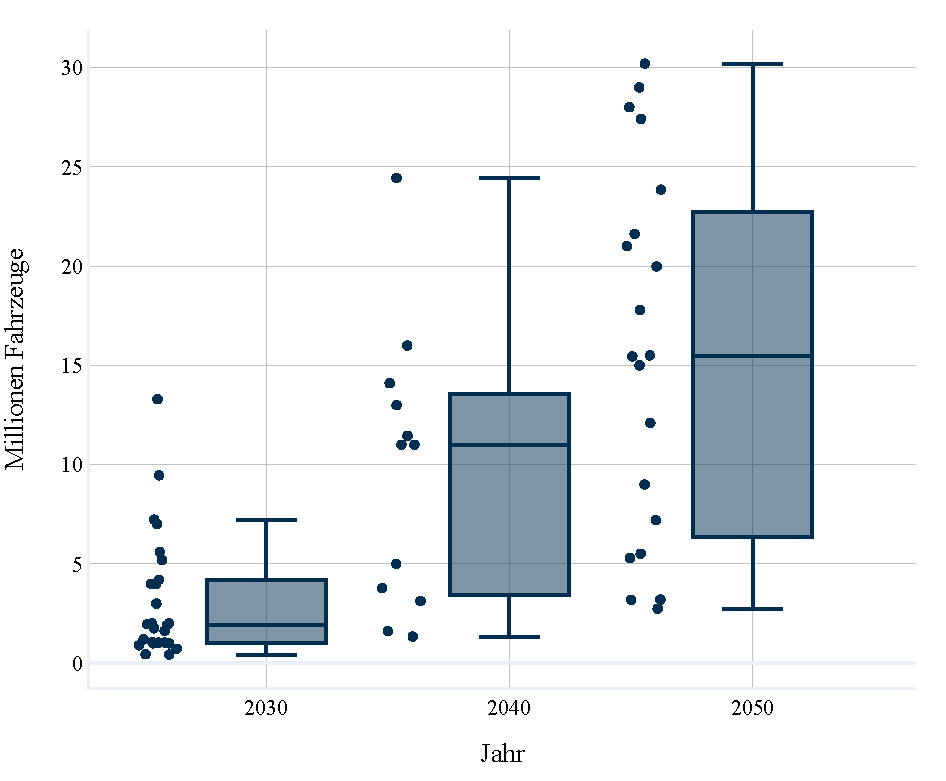
\includegraphics[width=\textwidth]{Bilder/RampUp-BEV-MA}
    \caption{Szenarienvergleich des Fahrzeugbestands von BEV bis zum Jahr \num{2050}}\label{fig:RampUpBEV}
\end{figure}

\clearpage

Neben dem Hochlauf an \glspl{BEV}, ist auch mit einem starken Hochlauf bei den \glspl{PHEV} zu rechnen.
Da ein Großteil der Fahrten von \glspl{PKW} eine Strecke von \SI{50}{\km} nicht überschreiten \cite{Agora2019}, können viele Fahrten auch von \glspl{PHEV} batterieelektrisch zurückgelegt werden.

\autoref{fig:RampUpPHEV} veranschaulicht die Annahmen der betrachteten Studien zum Fahrzeugbestand von \glspl{PHEV} bis zum Jahr \num{2050} als Box-Plot.
Die zugrundeliegenden Daten finden sich im Anhang in \autoref{tab:RampUpPHEV}.
Bei \glspl{PHEV} liegt der Anstieg im Fahrzeugbestand anfangs sogar höher als bei \glspl{BEV}.
So liegt der Median 2030 bereits bei \SI{3.7}{\MioFZs}.
Anschließend fällt der Fahrzeugbestand von \glspl{PHEV} hinter den der \glspl{BEV} zurück.
Bis \num{2040} steigt dieser auf \SI{8.2}{\Mio} und \num{2050} auf \SI{9.6}{\MioStk}.
Je nach Studie und Szenario sinkt der Fahrzeugbestand nach \num{2040} sogar wieder, da zur Erreichung der Klimaziele oder aus ökonomischen Gründen der Umstieg auf \glspl{BEV} als sinnvoller eingeschätzt wird.

\begin{figure}[H]
    \centering
    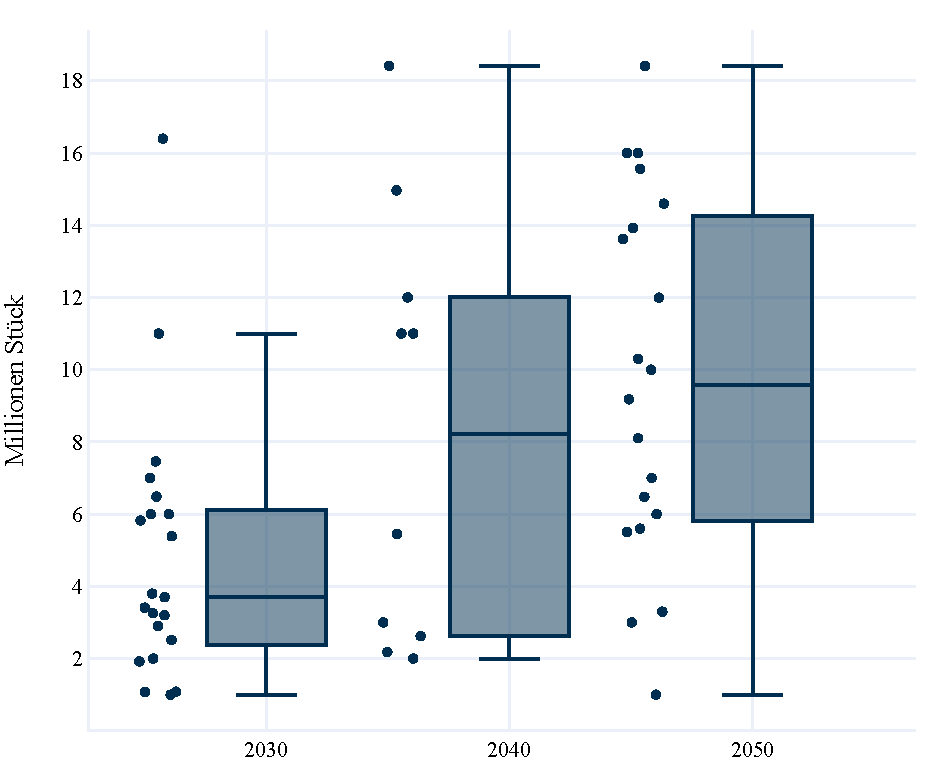
\includegraphics[width=\textwidth]{Bilder/RampUp-PHEV-MA}
    \caption{Szenarienvergleich des Fahrzeugbestands von PHEV bis zum Jahr \num{2050}}\label{fig:RampUpPHEV}
\end{figure}


\subsection{Methodik zur Modellierung der Elektromobilität}

Von den betrachteten Studien quantifizieren drei Studien den Netzausbaubedarf auf Verteilnetzebene und werden vertieft betrachtet.
Hierzu zählen die dena-Leitstudie \textit{Integrierte Energiewende} \cite{DEAGH2018}, die BCG Studie \textit{Klimapfade für Deutschland} \cite{BCG2018} und die Agora Studie \textit{Verteilnetzausbau für die Energiewende} \cite{Agora2019}.\medskip

In \autoref{fig:DSCAPEXMeta} werden die Ergebnisse der Studien für den Investitionsbedarf in die Verteilnetze bis zum Jahr \num{2050} aufgeteilt auf die drei Spannungsebenen \gls{NS}, \gls{MS} und \gls{HS} dargestellt.
Deutlich wird hierbei, dass die dena-Leitstudie die mit Abstand höchsten Kosten für den Netzausbau auf der \gls{NS}- und \gls{HS}-Ebene ermittelt.
Die Agora Studie untersucht hingegen die Netzausbaukosten nicht auf der \gls{HS}-Ebene, ermittelt jedoch die höchsten Ausbaukosten aller Studien auf der \gls{MS}-Ebene.
Ein direkter Vergleich der Ergebnisse ist jedoch nur bedingt möglich, da die drei Studien unterschiedliche Grundsätze für ihre Szenarien und die Bestimmung des Netzausbaubedarfs ansetzen.
An dieser Stelle sollen die Unterschiede und Gemeinsamkeiten zwischen den drei Studien in der Methodik zur Einbindung von \glspl{EPKW} in das Netzmodell dargestellt werden.

\begin{figure}[H]
    \centering
    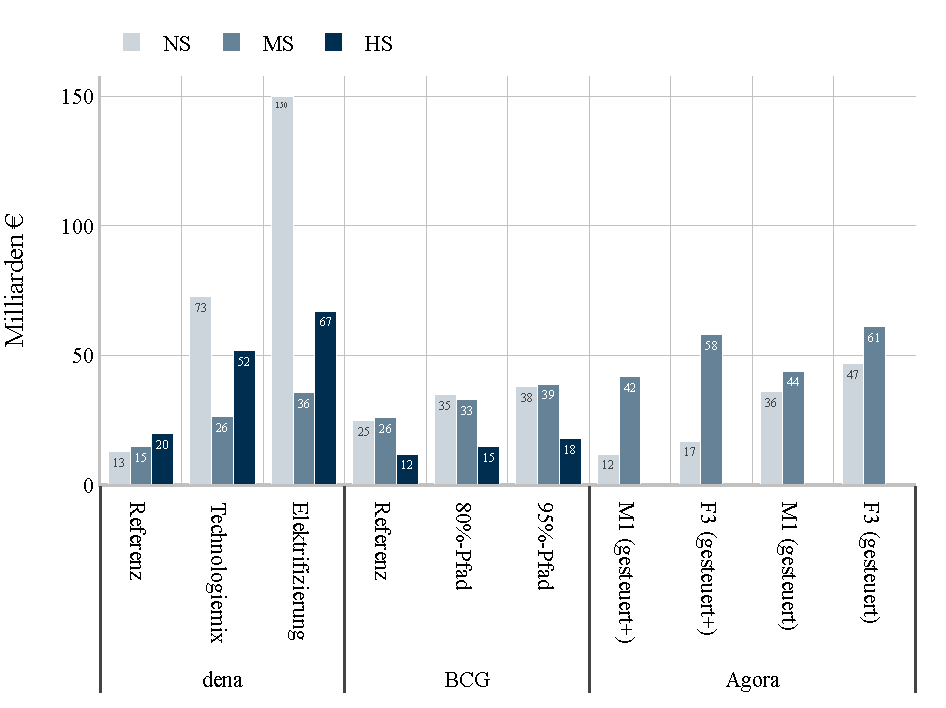
\includegraphics[width=\textwidth]{Bilder/DS-CAPEX-MA}
    \caption{Investitionsbedarf in die Verteilnetze bis zum Jahr \num{2050} je Spannungsebene}\label{fig:DSCAPEXMeta}
\end{figure}


\subsubsection{Bedarfsabschätzung}

Die Studien treffen bereits beim Hochlauf der Elektromobilität je Szenario stark unterschiedliche Annahmen, weshalb die Bedarfsabschätzung zwischen den Szenarien unterschiedlich ausfällt.
Die Zahlen für direktelektrifizierte Fahrzeuge in den ambitionierten Szenarien der Studien liegen mit minimal \SI{35}{\MioFZs} (BCG) und \SI{45}{\MioFZs} (Agora) allerdings in einer ähnlichen Dimension.
Der Verbrauch von \glspl{EPKW} wurde in der Agora Studie als homogen angenommen, während die dena-Leitstudie und die BCG Studie beim Verbrauch zwischen \glspl{BEV} und \glspl{PHEV} unterscheiden.
In der dena-Leitstudie und der BCG Studie wird eine Abschätzung der Veränderung im Mobilitätsverhalten vorgenommen, wodurch sich die Verkehrsleistung von \glspl{PKW} leicht verändert.
Demgegenüber wird bei der Agora Studie keine Veränderung der Verkehrsleistung gegenüber dem heutigen Stand angenommen.
Die Abschätzung der lokalen Belastungen durch die Elektromobilität erfolgt innerhalb der dena-Leitstudie und der Agora Studie anhand einer Evaluierung der Gleichzeitigkeit in Abhängigkeit vom Ladeort und der Anzahl der Fahrzeuge.
Die Evaluierung der Gleichzeitigkeit erfolgt in beiden Fällen anhand einer Monte-Carlo-Simulation simulierter Lastgänge, wobei das \SI{95}{\percent}-Quantil als auslegungsrelevant für die Netzplanung angesehen wird.
Die Agora Studie erweitert diese Annahme um die Abhängigkeit der Gleichzeitigkeit von der Ladeleistung.


\subsubsection{Ladestrategien}

Ein deutlicher Unterschied entsteht durch die Annahme der dena-Leitstudie, dass eine Steuerung der Ladevorgänge von neuen Verbrauchern nicht stattfindet.
Stattdessen geht die Studie davon aus, dass die zusätzliche Last durch \glspl{EPKW} und \glspl{WP} gleichzeitig mit der bisherigen Spitzenlast auftritt und der auslegungsrelevante Starklastfall somit deutlich erhöht wird.
Im Gegensatz zur dena-Leitstudie wird in der BCG-Studie von einem gesteuerten Laden der neuen Verbraucher ausgegangen.
Hierbei reagieren \SI{80}{\percent} der \glspl{EPKW} auf Strommarktsignale und werden nur geladen, wenn der \gls{SOC} auf weniger als \SI{50}{\percent} fällt oder eine lange Fahrt ansteht.
Bei der Agora Studie wird ein starker Fokus auf den Einfluss von aktiven netzdienlichen Ladestrategien auf den Netzausbaubedarf gelegt, indem eine Residuallastglättung innerhalb eines Netzgebietes angestrebt wird (gesteuert).
Ergänzend wurde ein erweitertes netzdienliches Ladekonzept (gesteuert\Plusdot) untersucht, welches zusätzlich zur Residuallastglättung die Verschiebung der Ladevorgänge über mehrere Standzeiten und eine Kappung von Lastspitzen erlaubt.
Das gesteuerte und gesteuert\Plus Laden werden in Form eines Reduktionsfaktors in der Netzplanung berücksichtigt.


\subsection{Abgrenzung zur vorliegenden Literatur}

In der ausgewerteten Literatur werden die Auswirkungen einer zunehmenden Netzintegration von \glspl{EPKW} auf die Verteilnetze in Deutschland bereits in ihrer Gesamtheit betrachtet.
In dieser Arbeit werden ergänzend die Auswirkungen auf fünf konkrete Referenznetzgebiete untersucht, welche jeweils stark unterschiedliche Charakteristika besitzen und grob in die Kategorien \gls{PV}-, Wind- bzw. Last-dominiert eingeteilt werden können.
Hierbei wird der Einfluss verschiedener netzdienlicher Ladestrategien untersucht und der Erfolg von präventiven und aktiven Ansätzen miteinander verglichen.
Somit soll eine Aussage darüber möglich werden, ob aktive Ansätze gegenüber präventiven Ansätzen einen wesentlichen Vorteil bieten.

In dieser Arbeit soll erweiternd zur vorliegenden Literatur ein verstärkter Fokus auf eine detaillierte Modellierung des direktelektrifizierten Fahrzeugbestandes mit verschiedenen Fahrzeugklassen von \glspl{EPKW} gelegt werden.
Weiterhin werden für die Untersuchung der Auswirkungen auf die Verteilnetze nicht feste Gleichzeitigkeiten und Reduktionsfaktoren ermittelt, sondern konkrete Bedarfszeitreihen verwendet.


\clearpage


\section{Methodik}\label{chap:Methodik}

Aufgrund ihrer Wichtigkeit für diese Arbeit werden zunächst die verwendeten Netztopologien sowie deren Clusterung zur Bestimmung repräsentativer Netze, anhand welcher die Untersuchungen vorgenommen werden, beschrieben und vorgestellt.
Anschließend werden mit Hilfe des Software Tools \gls{SIMBEV} Fahrtprofile von \glspl{EPKW} erstellt und die untersuchten Ladestrategien beschrieben.
Damit der Ladebedarf in die Netzmodelle integriert werden kann, muss dieser räumlich auf eine entsprechende georeferenzierte Ladeinfrastruktur verteilt werden.
Abschließend erfolgt eine Beschreibung der Methodik zur Bestimmung von Netzproblemen und der Ermittlung des Abregelungsbedarfs im Netzgebiet mit Hilfe des Open Source Tools \gls{EDISGO}.


\subsection{Verwendete Verteilnetztopologien}\label{chap:dingo_theo}

Eine der Grundlagen für die Nutzung des Netzplanungsinstruments \glspl{EDISGO} sind die zu untersuchenden Netztopologien der \gls{MS}- und \gls{NS}-Ebene.
Aufgrund der mangelnden Datenlagen von realen Netztopologien, wird auf synthetisch erzeugte Netztopologien zurückgegriffen, die innerhalb des \gls{OPENEGO} Projektes \cite{Mueller2019} mit Hilfe des Open Source Tools \gls{DINGO} erzeugt wurden.
Das Tool ist in der Lage ländliche und suburbane Netzstrukturen für Gesamtdeutschland zu synthetisieren und kann auf \textit{GitHub} \cite{dingo2019} öffentlich eingesehen und frei verwendet werden.
Weiterhin ist auf \textit{Read the Docs} \cite{dingo-docs2019} eine ausführliche Dokumentation nachzulesen.\medskip

Die Synthetisierung der Netztopologien ist nicht Teil dieser Arbeit und erfolgte innerhalb des \gls{OPENEGO} Projektes.
Die Netztopologien werden auf der Datengrundlage des Jahres \num{2015} gebildet und entsprechend ausgebaut.
Urbane Netzgebiete können derzeit nicht durch \gls{DINGO} abgebildet und können deshalb innerhalb dieser Arbeit nicht betrachtet werden.\medskip

In der konventionellen Netzplanung werden Betriebsmittel in der Regel überdimensioniert ausgelegt, um eine möglichst lange Betriebszeit zu garantieren.
Da die Netzgebiete des \gls{OPENEGO} Projektes so ausgebaut werden, dass die Versorgungsaufgabe des Jahres \num{2015} möglichst genau übernommen werden kann, werden die Netzgebiete zusätzlich ausgebaut.
Es wird angenommen, dass die Betriebsmittel mit einem Überdimensionierungsfaktor für die Scheinleistungs- bzw. Stromstärkenbelastbarkeit von mindestens \num{1.3} geplant und entsprechend ausgebaut werden.
Dies gilt sowohl für die Transformator-Stationen als auch die Kabel innerhalb des Netzgebietes.
Die verwendeten Betriebsmittel können der Dokumentation \glspl{EDISGO} \cite{edisgoDocs2017a} entnommen werden.
Sollte die maximal auftretende Scheinleistungsbelastung einer Transformator-Station größer sein als der größte verfügbare Transformator, so werden entsprechend benötigte Transformatoren parallel betrieben, um den Anforderungen gerecht zu werden.


\subsubsection{Mittelspannung}

Die einzelnen \gls{MS}-Netze werden alle als offene Ringnetze betrieben.
Im städtischen Bereich werden hauptsächlich Erdkabel mit einer Nennspannung von \SI{10}{\kv} eingesetzt, während im ländlichen Raum größtenteils Freileitungen mit einer Nennspannung von \SI{20}{\kv} eingesetzt werden. \cite{Mueller2019}\medskip

Die Modellierung der Mittelspannungstopologie erfolgt als Tourenplanungsproblem (\gls{CVRP}) in Kombination mit der Beachtung der historisch lastorientierten Entwicklung und den Planungsprinzipien von Verteilnetzen.
Ein besonderer Fokus liegt dabei auf der Beachtung von Leitungsüberlastungen und Verletzungen des Spannungsbandes.
Eine genau Beschreibung der Methodik findet sich in \textit{The eGo grid model} \cite{Amme2018}.


\subsubsection{Niederspannung}

Die \gls{NS}-Ebene wird mit Hilfe von \num{46} Referenznetzsträngen synthetisiert und die einzelnen \gls{NS}-Netze werden als Strahlennetz abgebildet.
Die Referenznetzstränge stehen jeweils repräsentativ für eine bestimmte Anzahl an Hausanschlüssen innerhalb einer Netzklasse, wobei letztere nach Land-, Dorf- und Vorstadtnetzen unterschieden werden.
Auf Grundlage der Anzahl an Hausanschlüssen je Ortsnetzstation wird ein \gls{NS}-Netz einer Netzklasse zugeordnet.
Die verschiedenen Referenznetzstränge der entsprechenden Netzklasse werden anschließend so miteinander kombiniert, dass für die entsprechende Anzahl an Hausanschlüssen ein typisches Netz generiert wird. \cite{Mueller2019}


\subsubsection{K-Means-Clustering}

Innerhalb Deutschlands wurden insgesamt \num{3354} Netzgebiete \cite{Schachler} identifiziert und mit Hilfe des Open Source Tools \gls{DINGO} synthetisiert.
Bei der Synthese der Netztopologien wurde auf eine hohe räumliche und zeitliche Auflösung des Netzdatenmodells geachtet.
Die große Anzahl an Netzgebieten und die hohe Auflösung führen zu inakzeptabel hohen Rechenzeiten.
Um die Komplexität des Modells zu reduzieren, wurden in  mit Hilfe des \kmeans Referenznetzgebiete ausgewählt, die stellvertretend für eine möglichst große Zahl an Netzgebieten stehen.
Das \kmean wurde im Rahmen des \gls{OPENEGO} Projektes \cite{Mueller2019} entwickelt und wurde innerhalb \textit{E-Mobility Study} \cite{Schachler} unverändert angewendet.
Innerhalb dieser Arbeit soll eine Teilmenge der ermittelten \num{15} Netzgebiete mit stark unterschiedlichen Charakteristiken untersucht werden.
An dieser Stelle soll das grundlegende Vorgehen erläutert werden. \medskip

Grundlage des \kmeans bildet der \gls{EMA} des Python Paketes \textit{scikit learn} \cite{scikit-learn2011}.
Hierbei kann jedes \gls{MS}-Netzgebiet durch die Definition mehrerer numerischer Attribute als Punkt im mehrdimensionalen Raum beschrieben werden.
Der Algorithmus bildet anschließend eine vorgegebene Anzahl an Clustern $k$ durch die Minimierung der Summe der quadrierten gewichteten euklidischen Abstände zwischen den originalen Netzknoten und den Clusterzentren.
Für die Bildung der Cluster werden die folgenden vier Attribute verwendet, um die einzelnen \gls{MS}-Netzgebiet zu repräsentieren:

\begin{itemize}
	\item Entwicklung der installierten \gls{PV}-Kapazitäten
	\item Entwicklung der installierten Wind-Kapazitäten
	\item Spitzenlast durch \glspl{WP}
	\item Spitzenlast durch \gls{EPKW}
\end{itemize}

Die Regionalisierung der \gls{PV}-, Wind- und \gls{WP}-Kapazitäten erfolgt nach \autoref{chap:Szenariorahmen}.
Da die Simulation aller \gls{EPKW} aufgrund der großen Anzahl nicht für jedes \gls{MS}-Netzgebiet durchgeführt werden kann, muss die Spitzenlast durch \gls{EPKW} bereits im Voraus abgeschätzt werden.
So wird angenommen, dass nach den Hochlaufzahlen des Antriebswende-Szenarios jeder \gls{PKW} durch einen \gls{EPKW} ersetzt wird und jeder \gls{EPKW} im Jahr \SI{12000}{\km} zurücklegt.
Anhand eines durchschnittlichen Verbrauches von \SI{20}{\kwhkm} wird anschließend der Ladebedarf je Gemeinde abgeschätzt.
Anschließend wird der Ladebedarf mit einem beispielhaften Lastprofil auf die Netzgebiete anhand des Flächenanteils der Gemeinde im Netzgebiete verteilt.


\subsubsection{Auswahl repräsentativer Verteilnetztopologien}

Auf der \gls{MS}-Ebene gibt es \num{3354} Netzgebiete mit einer mittleren Fläche von \SI{99}{\km\squared}.
\autoref{fig:grid_176_map} zeigt den Aufbau eines beispielhaften Mittelspannungsnetzes, welches mit Hilfe von \gls{DINGO} erzeugt wurde und innerhalb dieser Arbeit untersucht wird.

\begin{figure}[H]
    \centering
    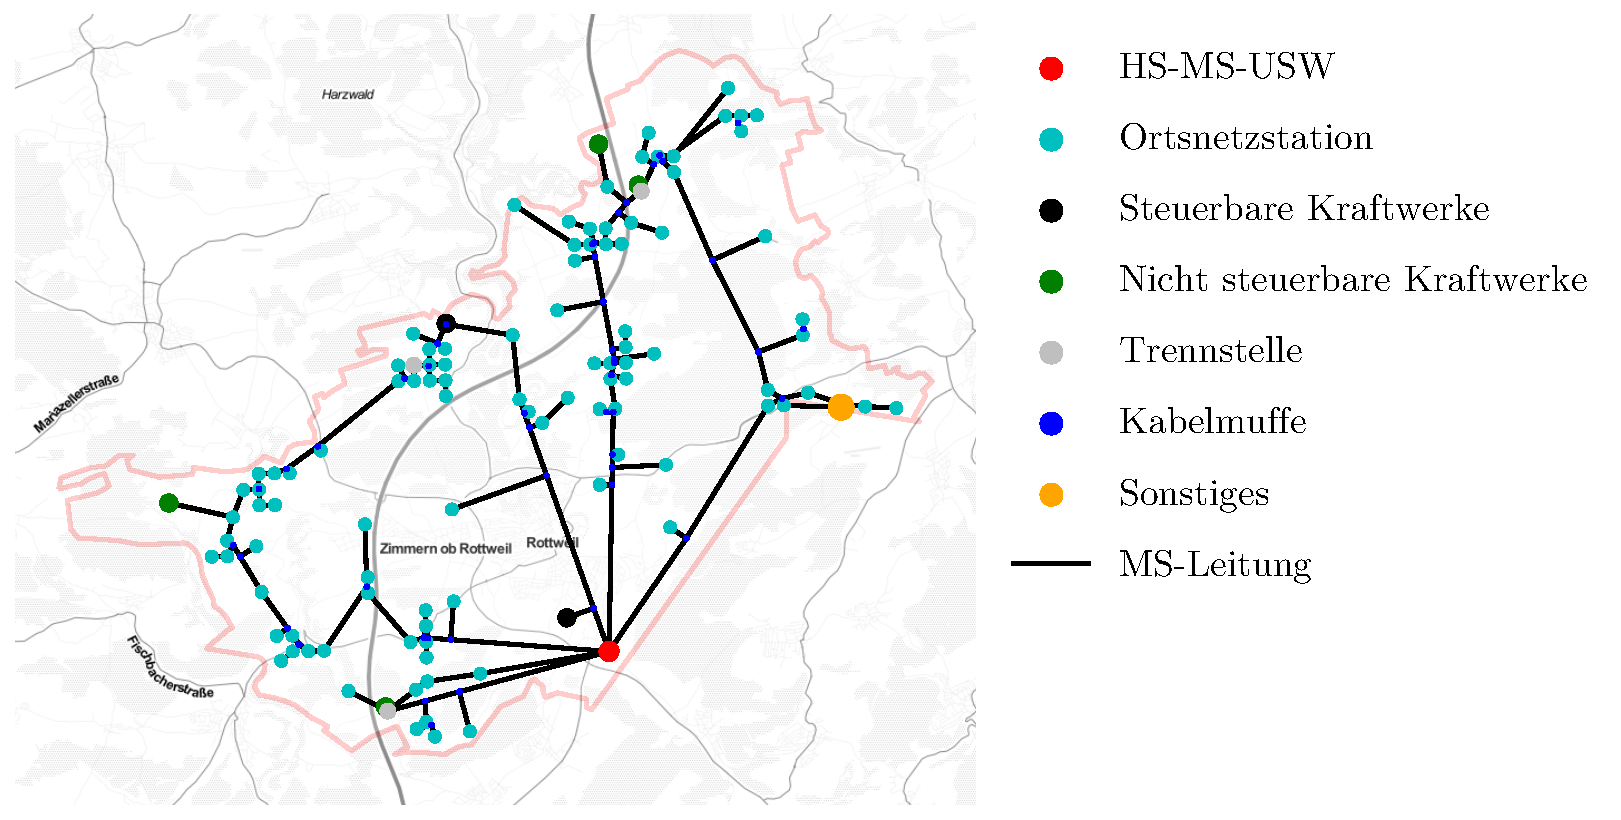
\includegraphics[width=\textwidth]{Bilder/grid_176_map}
    \caption{Beispielhafte Darstellung des MS-Netzes \num{176} mit allen Umspannwerken, Erzeugerkapazitäten und sonstigen Betriebsmitteln}\label{fig:grid_176_map}
\end{figure}

Um mit dieser Arbeit eine Ergänzung zur \textit{E-Mobility Study} \cite{Schachler} zu liefern, werden die Ergebnisse des Clusterings aus der \textit{E-Mobility Study} übernommen und von den \num{15} identifizierten repräsentativen Netzgebieten eine Teilmenge untersucht.
So werden jeweils zwei Netzgebiete der Kategorien \gls{PV}- und Wind-dominiert und ein Netzgebiet der Kategorie Last-dominiert ausgewählt, die stellvertretend für viele Netzgebiete stehen.
Auf diese Weise wird sichergestellt, dass die Effekte der Netzintegration der Elektromobilität für unterschiedliche Netzklassen aufgezeigt werden können.
Insgesamt werden somit fünf Netzgebiete untersucht, die repräsentativ für \num{1495} der \num{3354} Netzgebiete stehen.
In \autoref{tab:grid_IDs} werden die untersuchten \gls{MS}-Netzgebiet nach ihrem \gls{ID} kategorisiert und die Anzahl an repräsentierten Netzgebieten dargestellt, wobei der Index der Netz \glspl{ID} für die jeweilige Netzkategorie steht.

{
\renewcommand{\arraystretch}{1.2}% grßerer Zeilenabstand
\sisetup{range-phrase=~{--}~}% Gedankenstrich statt "bis" bei SIrange
\begin{table}[H]
	\begin{center}
		\caption{Anzahl der repräsentierten Netzgebiete und Kategorie der untersuchten Mittelspannungsnetze}
		\begin{tabu} to \textwidth {X[1] X[1] X[1, r] }
			\hline
			Netz ID    & Kategorie      & Anzahl repräsentierter Netze \\ \hline
			\num{176}  & PV-dominiert   & \num{413}                    \\
			\num{1056} & PV-dominiert   & \num{197}                    \\
			\num{1690} & Wind-dominiert & \num{141}                    \\
			\num{1811} & Wind-dominiert & \num{78}                     \\
			\num{177}  & Last-dominiert & \num{666}                    \\
			\num{2534} & Last-dominiert & \num{347}                    \\ \hline
		\end{tabu}
		\label{tab:grid_IDs}
	\end{center}
	\vspace{-3mm}%Put here to reduce too much white space after your table
\end{table}
}

In \autoref{fig:bar_representatives} werden die wichtigsten Charakteristika der untersuchten \gls{MS}-Netzgebiete dargestellt.
Hierzu zählen die installierten \gls{PV}- und Wind-Kapazitäten, sowie die Spitzenlast der \glspl{EPKW} beim Referenz-Laden (s. \autoref{chap:theo_strategies}) im Antriebswende-Szenario und des konventionellen Stromverbrauches inklusive \glspl{WP}.
Weiterhin wird in \autoref{fig:map_representatives} eine Karte der repräsentierten \gls{MS}-Netzgebiete, eingeteilt in die Kategorien \gls{PV}-, Wind- und Last-dominiert, dargestellt.

\begin{figure}[H]
    \centering
    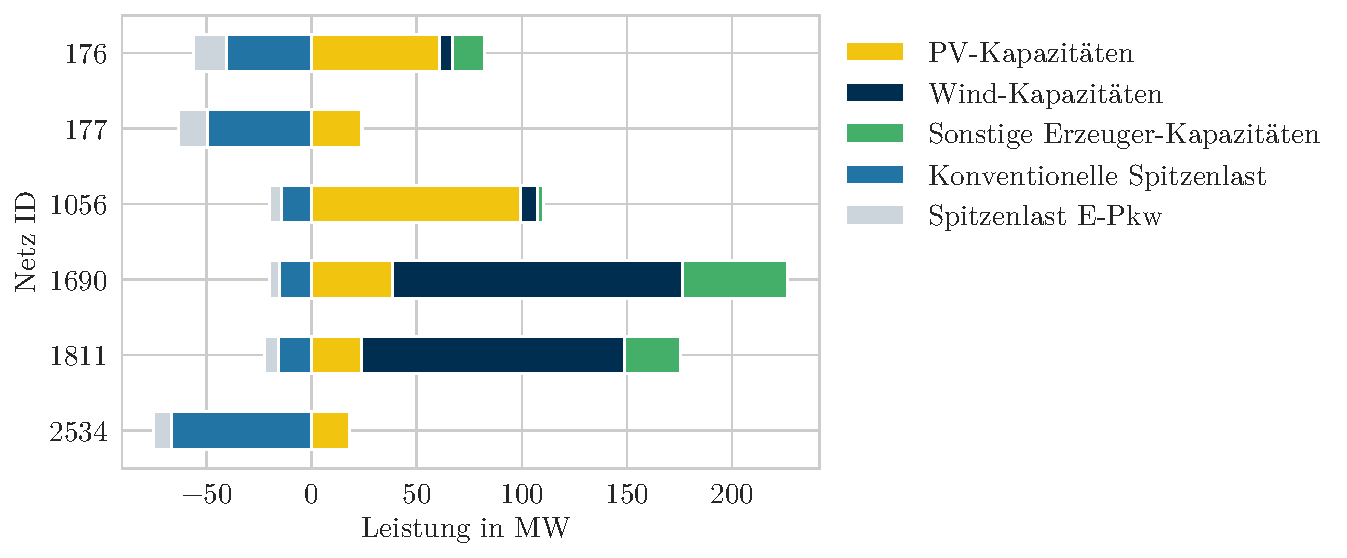
\includegraphics[width=\textwidth]{Bilder/Installed_cap_peak_load_representatives}
    \caption{Kumulierte Wirkleistung von PV-, Wind- und sonstigen Erzeuger-Kapazitäten sowie die kumulierte konventionelle und mobilitätsbedingte Spitzenlast in den Referenznetzgebieten}\label{fig:bar_representatives}
\end{figure}

\begin{figure}[H]
    \centering
    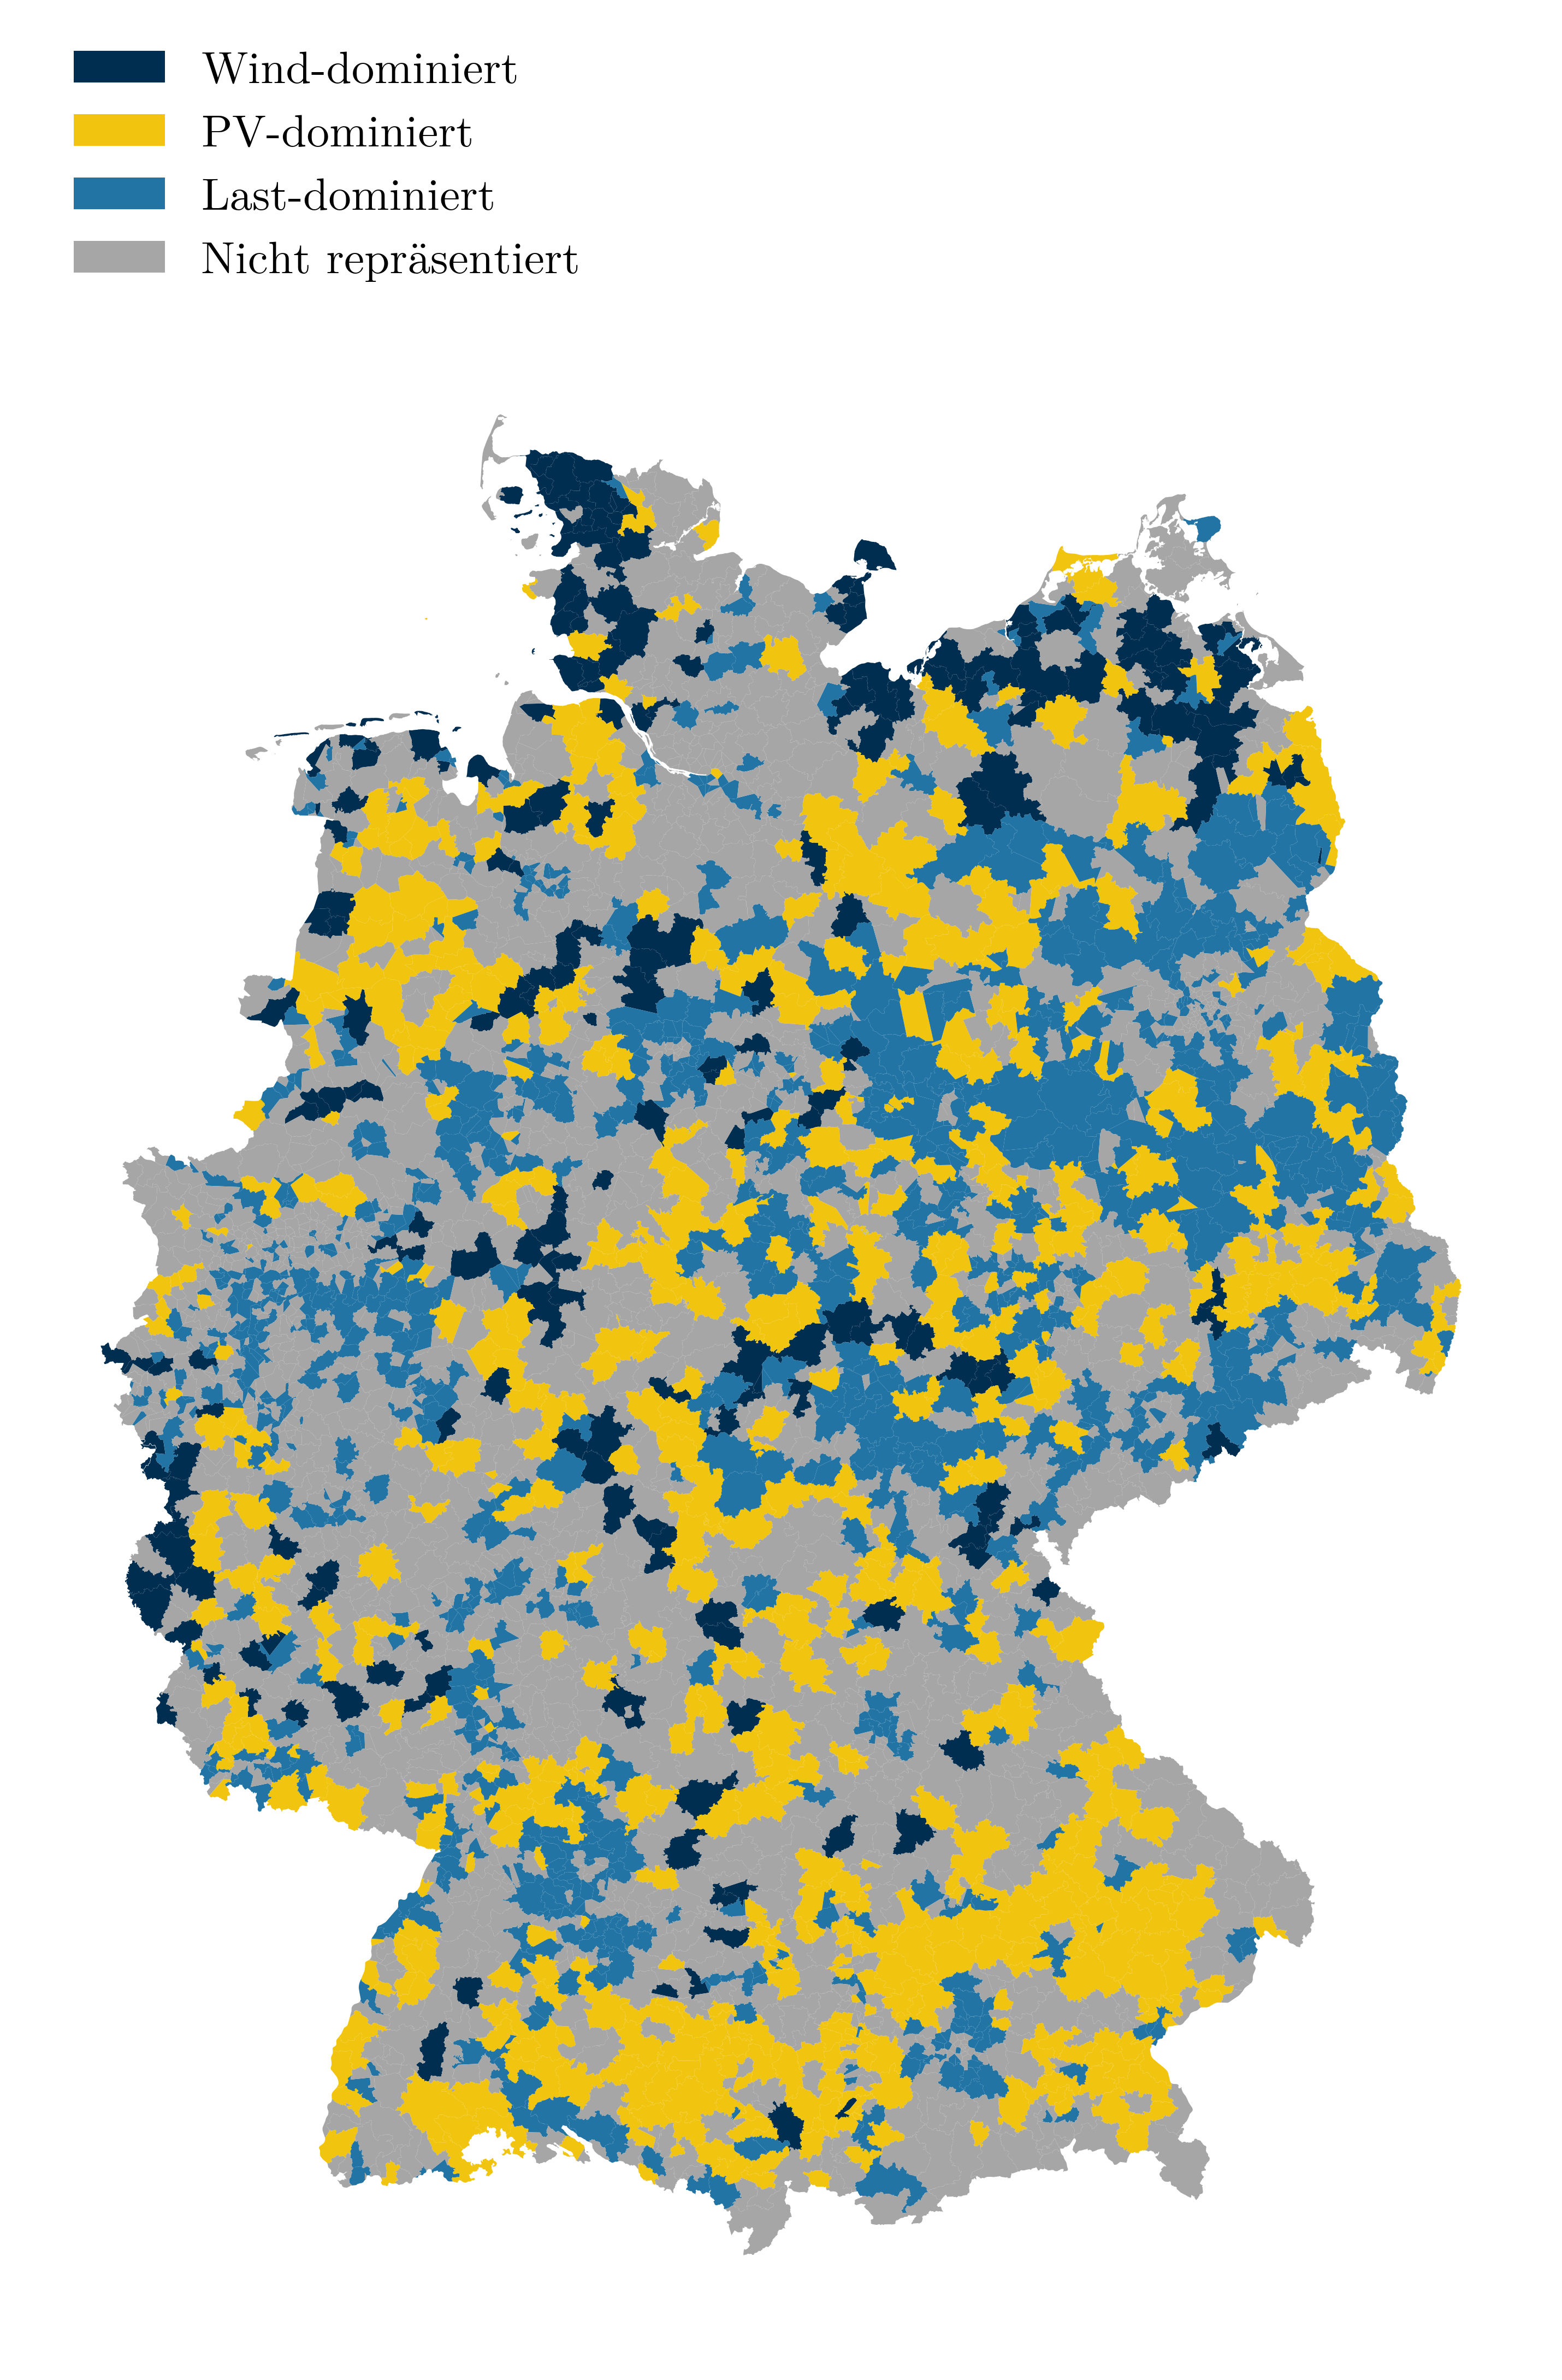
\includegraphics[width=\textwidth]{Bilder/clusters_representatives}
    \caption{Repräsentierte Netzgebiete in Deutschland}\label{fig:map_representatives}
\end{figure}


\subsection{Erstellung der Fahrtprofile der E-Pkw}\label{chap:simbev_theo}

Mit Hilfe des im Rahmen dieser Arbeit mitentwickelten Software Tools \gls{SIMBEV} können die Fahrtprofile für eine beliebige Anzahl an \glspl{EPKW} verschiedener Fahrzeugklassen erstellt werden.
Grundlage von \gls{SIMBEV} bildet die Befragung \gls{MID} \cite{ISGH2017}.
Nachfolgend wird zunächst die Datengrundlage und anschließend die Methodik zur Erstellung der Fahrtprofile mit Hilfe von \gls{SIMBEV} beschrieben.


\subsubsection{Mobilität in Deutschland}\label{chap:MID}

Das Ziel der Befragung \gls{MID} \cite{ISGH2017} ist es, eine Datengrundlage für das alltägliche Mobilitätsverhalten von Personen und Haushalten über ein Jahr zu bilden.
Für diese Arbeit sind vor allem die Erhebungen der sieben Hauptwegezwecke entscheidend.
Diese sind: \textit{Arbeit}, \textit{dienstlich}, \textit{Ausbildung}, \textit{Einkauf}, \textit{Erledigung}, \textit{Freizeit} und \textit{Begleitung}.
In \autoref{tab:wegezweck} wird die prozentuale Aufteilung der Hauptwegezwecke am \gls{PKW}-Verkehrsaufkommen in Wegen beschrieben.

{
\renewcommand{\arraystretch}{1.2}% grßerer Zeilenabstand
\sisetup{range-phrase=~oder~}
\begin{table}[H]
	\begin{center}
		\caption{Anteil der Fahrtzwecke am Pkw-Verkehrsaufkommen (Wege)}
		\begin{tabu} to 0.6\textwidth {X[1] X[1, r]}
			\hline
			Wegezweck  & Verkehrsaufkommen \\ \hline
			Arbeit     & \SI{28}{\percent} \\
			dienstlich & \SI{21}{\percent} \\
			Ausbildung & \SI{1}{\percent}  \\
			Einkauf    & \SI{8}{\percent}  \\
			Erledigung & \SI{13}{\percent} \\
			Freizeit   & \SI{24}{\percent} \\
			Begleitung & \SI{6}{\percent}  \\ \hline
            \multicolumn{2}{l}{Quelle: \cite{Nobis2019}}
		\end{tabu}
		\label{tab:wegezweck}
	\end{center}
	\vspace{-3mm}%Put here to reduce too much white space after your table
\end{table}
}

Der Wegezweck \glqq Begleitung\grqq{} wird innerhalb von \gls{SIMBEV} nicht abgebildet, da hierfür keine zusätzliche Fahrt angetreten wird.
Der Rückweg der Wegezwecke wird getrennt als Wegezweck \nH berücksichtigt, da dem Laden zu Hause eine besonders wichtige Rolle zukommt.
Weiterhin dient \gls{SIMBEV} nur der Erstellung von Fahrtprofilen für \glspl{PKW}, weshalb ausschließlich die Ergebnisse der Befragung zu Fahrten mit dem Hauptverkehrsmittel \gls{PKW} betrachtet werden.
Die für diese Arbeit entscheidenden Befragungsergebnisse sind somit die Fahrtzeiten, Fahrtstrecken und anschließenden Standzeiten je Hauptwegezweck für Fahrten mit \glspl{PKW}.
Bei den Befragungsergebnissen kann zusätzlich zwischen den in \autoref{tab:RegioStaR} aufgelisteten \glspl{REGIOSTAR} unterschieden werden.

{
\renewcommand{\arraystretch}{1.2}% grßerer Zeilenabstand
\sisetup{range-phrase=~oder~}
\begin{table}[H]
	\begin{center}
		\caption{Regionalstatistische Raumtypologien 7}
		\begin{tabu} to \textwidth {X[1] X[2]}
			\hline
			Raumtypologie ID	 	& Regionalstatistische Raumtypologie                        \\ \hline
			\num{71}       			& Metropolen                                                \\
			\num{72}       			& Regiopolen und Großstädte                                 \\
			\num{73}       			& Mittelstädte, städtischer Raum einer Stadtregion          \\
			\num{74}       			& Kleinstädtischer dörflicher Raum einer Stadtregion        \\
			\num{75}       			& Zentrale Städte einer Ländlichen Region                   \\
			\num{76}       			& Mittelstädte, städtischer Raum                            \\
			\num{77}       			& Kleinstädtischer, dörflicher Raum einer Ländlichen Region \\ \hline
            \multicolumn{2}{l}{Quelle: \cite{BMVI2020}}
		\end{tabu}
		\label{tab:RegioStaR}
	\end{center}
	\vspace{-3mm}%Put here to reduce too much white space after your table
\end{table}
}

Mit Hilfe dieser detaillierteren Unterscheidung kann ein raumtypenspezifisches Fahrverhalten abgebildet werden, welches eine erhöhte Genauigkeit bei der Erstellung der Fahrtprofile nach sich zieht.
In \autoref{tab:RegioStaR} wird die mittlere Fahrleistung pro Person und pro \gls{PKW} sowie die mittlere Fahrtweite von \gls{PKW}-Fahrten nach Raumtyp dargestellt, um die Differenzen zwischen den einzelnen Raumtypen aufzuzeigen.

{
\renewcommand{\arraystretch}{1.2}% grßerer Zeilenabstand
\sisetup{range-phrase=~oder~}
\begin{table}[H]
	\begin{center}
		\caption{Mittlere jährliche Fahrleistung und mittlere Fahrweite für Pkw}
		\begin{tabu} to 0.7\textwidth {X[0.5] X[1, r] X[1, r]}
			\toprule
			ID       & Mittlere Fahrleistung & Mittlere Fahrtweite \\ \midrule
			\num{71} & \SI{13200}{\km}       & \SI{17}{\km}        \\
			\num{72} & \SI{14100}{\km}       & \SI{15}{\km}        \\
			\num{73} & \SI{14600}{\km}       & \SI{15}{\km}        \\
			\num{74} & \SI{15800}{\km}       & \SI{16}{\km}        \\
			\num{75} & \SI{14300}{\km}       & \SI{15}{\km}        \\
			\num{76} & \SI{14500}{\km}       & \SI{14}{\km}        \\
			\num{77} & \SI{15900}{\km}       & \SI{16}{\km}        \\ \bottomrule
            \multicolumn{2}{l}{Quelle: \cite{Nobis2019}}
		\end{tabu}
		\label{tab:mid_fahrleistung}
	\end{center}
	\vspace{-3mm}%Put here to reduce too much white space after your table
\end{table}
}


\subsubsection{simBEV}

Die Fahrtprofile werden über einen probabilistischen Ansatz auf Grundlage der Befragung \gls{MID} erstellt.
Dabei erhält jeder simulierte Zeitschritt eine Wahrscheinlichkeit für einen bestimmten Wegezweck, um eine Fahrt zu beginnen.
Wird eine Fahrt ausgelöst, wird abhängig vom Wegezweck und Regionstyp der Fahrt, ebenfalls probabilistisch, eine Streckenlänge und eine anschließende Standzeit zugeteilt.
Der hierbei entstehende Verbrauch des \gls{EPKW} muss anschließend gedeckt werden.
Ob am Zielort ein Ladevorgang stattfindet, hängt vom \gls{SOC} des \gls{EPKW} und dem Vorhandensein eines Ladepunktes ab.
Mit Hilfe der Wahrscheinlichkeiten aus \autoref{tab:WegezweckProbability2050} wird die Verfügbarkeit eines Ladepunktes am Zielort und die entsprechende Ladeleistung ermittelt.
Ladepunkte besitzen pauschal einen Wirkungsgrad von \SI{90}{\percent} \cite{EliaGroup2020}.
Die Bestimmung des Vorhandenseins eines Ladepunktes für die Wegezwecke \nH und \Arbeit erfolgt je \gls{EPKW} einmalig.
Für alle anderen Wegezwecke erfolgt jedesmal eine erneute Bestimmung.
Wird dem Zielort ein Ladepunkt zugeordnet, wird davon ausgegangen, dass die Fahrzeugnutzerin oder der Fahrzeugnutzer einen Ladevorgang erst ab einem bestimmten \gls{SOC} einleitet, da dies einen zusätzlichen Aufwand für die Nutzerin oder den Nutzer bedeutet.
Dabei wird angenommen, dass das Laden des \gls{EPKW} am Wohnort und am Arbeitsplatz bereits ab einem \gls{SOC} von \SI{95}{\percent} stattfindet.
Im öffentlichen Raum bedeutet das Anfahren und der Anschluss an einen Ladepunkt einen größeren Aufwand für die Nutzerin oder den Nutzer als im privaten Raum.
Deshalb wird angenommen, dass oberhalb eines \glspl{SOC} von \SI{80}{\percent} keine Ladevorgänge stattfinden.
Es gilt, je niedriger der \gls{SOC}, desto wahrscheinlicher ist es, dass die öffentliche Ladeinfrastruktur genutzt wird.
Ab einem \gls{SOC} von \SI{50}{\percent} findet, wann immer möglich, eine Ladung statt.
Zwischen den beiden Stützwerten erfolgt eine lineare Interpolation, welche in \autoref{fig:soc_charging_prob} visualisiert wird.

\begin{figure}[H]
    \centering
    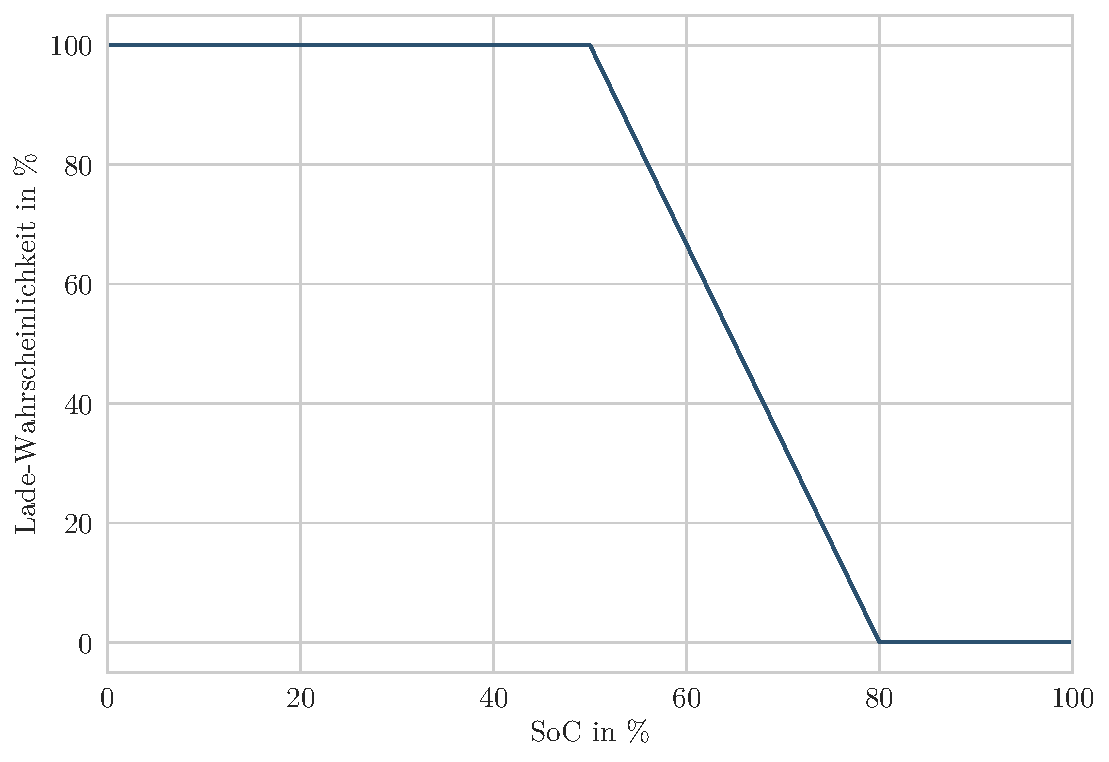
\includegraphics[width=0.9\textwidth]{Bilder/soc_charging_prob}
    \caption{Abhängigkeit der Ladewahrscheinlichkeit vom SoC an öffentlichen Standorten}\label{fig:soc_charging_prob}
\end{figure}

Schnellladeinfrastruktur besitzt aufgrund des zusätzlichen Fahrt- und Zeitaufwandes eine geringere Attraktivität für den Nutzer.
Deshalb wird eine Schnellladung in dieser Simulation nur dann ausgelöst, wenn es wirklich nötig ist.
Sinkt der \gls{SOC} eines \gls{EPKW} unter \SI{20}{\percent}, wird eine Schnellladestation angefahren und der \gls{EPKW} für \SI{15}{\Minuten} geladen.
Im Unterschied zu \glspl{BEV} können \glspl{PHEV} auch mit einem \gls{SOC} von \SI{0}{\percent} ihre Fahrt mit Hilfe des Verbrennungsmotors fortsetzen.
Aus diesem Grund wird bei \glspl{PHEV} kein Schnellladevorgang ausgelöst.\medskip

Derzeit können mit \gls{SIMBEV} nur Fahrtprofile mit einer Länge von einer Woche simuliert werden.
Da hierdurch ein Initialproblem eines vollständig geladenen Fahrzeugbestandes am ersten Tag der Simulation dominant hervortritt, wird zu Beginn der Simulation \SI{15}{\percent} der \glspl{EPKW} ein zufälliger \gls{SOC} zwischen \SIrange[range-phrase=~bis~]{30}{100}{\percent} zugeordnet.
Um abschließend ein Fahrtprofil für ein ganzes Jahr zu erhalten, werden die Fahrtprofile solange mit sich selbst verlängert und logisch verknüpft, bis die gewünschte Länge erreicht wird.


\subsubsection{Regionalisierung des Fahrzeugbestandes}

Um die Anzahl an \glspl{EPKW} je \gls{MS}-Netzgebiet zu bestimmen, muss der Gesamtbestand an \glspl{EPKW} je Szenario (s. \autoref{tab:SzenarienRampUp} und \autoref{tab:CarSplit}) regionalisiert werden.
Die Regionalisierung der \glspl{EPKW} findet vorerst auf Ebene der Landkreise statt.
Als Grundlage hierfür dient der aktuelle \gls{PKW}-Bestand nach Zulassungsbezirken \cite[][Stand: \DTMdate{2020-01-01}]{KBAPLZ2020}.
Es wird davon ausgegangen, dass es zu keiner Verschiebung des Bestandanteils zwischen den Zulassungsbezirken kommt.
Dies bedeutet, dass die Gesamtanzahl der \glspl{EPKW} je Fahrzeugklasse und Szenario entsprechend des heutigen Bestandes anteilig verteilt wird.
Die Aufteilung der \glspl{EPKW} in Klassen erfolgt anhand der Einteilung des \gls{PKW}-Bestandes in Hubraum-Klassen, welche ebenfalls dem \gls{PKW}-Bestand nach Zulassungsbezirken entnommen werden können.\medskip

Die geographische Einteilung der Landfläche in \glspl{REGIOSTAR} erfolgt auf Gemeindeebene, weshalb eine weitere Regionalisierung der \glspl{EPKW} innerhalb eines Landkreises auf die jeweiligen Gemeinden notwendig ist.
Da auf Gemeindeebene keine Daten zum \gls{PKW}-Bestand vorliegen, erfolgt die Regionalisierung anhand der Bevölkerungszahl der Gemeinden.
Die Grundlage hierfür bildet der Datensatz \textit{Gemeindegrenzen 2017 mit Einwohnerzahl} \cite[][Stand: \DTMdate{2017-12-31}]{EDG2020}.
Die Verteilung der Anzahl der \glspl{EPKW} erfolgt proportional zur Bevölkerungszahl in der jeweiligen Gemeinde.
Jedes \gls{MS}-Netzgebiet streckt sich dabei in der Regel über mehrere Gemeinden, wobei einzelne Gemeinden auch nur anteilig innerhalb eines Netzgebietes liegen können.\medskip

Um abschließend die Fahrtprofile erzeugen zu können, muss jeder Gemeinde eine \gls{REGIOSTAR} Nummer zugeordnet werden.
Die entsprechende Zuordnung für das Jahr \num{2018} kann dem Datensatz \textit{Referenzdateien zur regionalstatistischen Raumtypologie} \cite[][Stand: \DTMdate{2018-01-01}]{BMVIa2020} entnommen werden.


\subsection{Räumliche Verteilung der Ladevorgänge}\label{chap:theo_distribution}

Die räumliche Verteilung der Ladevorgänge innerhalb eines geographischen Gebietes kann starken Einfluss auf die Auswirkungen der Netzintegration von \glspl{EPKW} haben.
So können beispielsweise regionale Konzentrationen von Ladepunkten einzelne Leitungen stark beanspruchen und den Netzausbaubedarf erhöhen.\medskip

Innerhalb dieser Arbeit erfolgt die Verteilung der Ladevorgänge immer innerhalb des untersuchten geographischen Gebietes.
In der Realität wird es vorkommen, dass \glspl{EPKW} außerhalb ihres während der Regionalisierung zugewiesenen geographischen Gebietes geladen werden.
Dies betrifft vor allem den Pendel- und Urlaubsverkehr.
Ein Laden in anderen geographischen Gebieten oder das Laden von \glspl{EPKW} aus anderen Gebieten im untersuchten Gebiet kann nicht abgebildet werden.
Es wird davon ausgegangen, dass sich die hierdurch entstehende Verschiebung des Ladebedarfs zwischen den einzelnen Gebieten ungefähr ausgleicht und keinen großen Einfluss auf die Ergebnisse dieser Untersuchung hat.
Es ist vorstellbar, dass in einzelnen Fällen auch größere Verschiebungen entstehen, wenn beispielsweise innerhalb eines geographischen Gebietes ein großer Ladepark gebaut wird oder ein großes Unternehmen ansässig ist, welches als Anlaufpunkt für eine Vielzahl von \glspl{EPKW} aus anderen Gebieten dient. 
Ein solcher Fall kann somit nicht innerhalb dieser Arbeit abgebildet werden.\medskip

Grundlage für die Ermittlung von möglichen Standorten mitsamt einer Gewichtung bietet eine geoinformatische Auswertung der untersuchten geographischen Gebiete.
Das hierfür verwendete Software Tool wird unabhängig von der vorliegenden Arbeit am \textit{Reiner Lemoine Institut} entwickelt und ist noch nicht veröffentlicht.
Erweiternd zu der Identifizierung der möglichen Ladeinfrastruktur wurde innerhalb dieser Arbeit eine Methodik für die Zuteilung der Ladevorgänge auf die Ladeinfrastruktur entwickelt.


\subsubsection{Private Ladeinfrastruktur}

Die private Ladeinfrastruktur beinhaltet alle Ladevorgänge, die am Eigenheim, in Wohnanlagen oder auf dem Firmenparkplatz stattfinden.
Eine genaue Beschreibung der \UCs findet sich in \autoref{chap:Szenariorahmen}.
Um mögliche Standorte für die Ladeinfrastruktur am Eigenheim oder in Wohnanlagen identifizieren zu können, wird die Anzahl an Wohneinheiten auf einem \SI{100 x 100}{\m} Raster aus dem \textit{Zensus 2011} \cite{StatistischesBundesamt2011} verwendet.
So wird jedem Raster mit mehr als einer Wohneinheit und einer Einwohnerzahl größer Null ein möglicher Anschlusspunkt für Ladeinfrastruktur zugeordnet und anhand der Gesamtanzahl von Wohneinheiten im Raster gewichtet. \medskip

Für private Ladeinfrastruktur auf Firmenparkplätzen werden die Klassifizierungen der Landflächen nach Nutzungsart der \gls{OSM} \cite{OpenStreetMapFoundation} verwendet.
Hierbei wird jeder Landfläche mit der Nutzungsart \textit{commercial}, \textit{retail} oder \textit{industrial} ein möglicher Anschlusspunkt für Ladeinfrastruktur zugeordnet.
Die Gewichtung erfolgt anhand der Fläche des Gebietes multipliziert mit einem Flächennutzungsfaktor.
Der Flächennutzungsfaktor liegt für \textit{commercial} bei \num{3}, für \textit{retail} bei \num{2} und für \textit{industrial} bei \num{1}.


\subsubsection{Öffentliche Ladeinfrastruktur}

Die öffentliche Ladeinfrastruktur beinhaltet die Ladeinfrastruktur, die nicht der privaten Ladeinfrastruktur zugeordnet werden kann.
Grundsätzlich lässt sich hierbei zwischen Normal- und Schnellladeinfrastruktur unterscheiden.
Für die Normalladeinfrastruktur wird allen \glspl{POI} aus der \gls{OSM} \cite{OpenStreetMapFoundation} in dem untersuchten Gebiet jeweils ein möglicher Anschlusspunkt für Ladeinfrastruktur zugeordnet.
Die Gewichtung der Anschlusspunkte erfolgt hierbei anhand der Gesamtanzahl an \glspl{POI} in der Nähe des Anschlusspunktes.\medskip

Für Schnellladeinfrastruktur wird jeder Tankstelle aus der \gls{OSM} \cite{OpenStreetMapFoundation} im untersuchten Gebiet jeweils ein Anschlusspunkt zugeordnet.
Liegt innerhalb des Gebietes keine Tankstelle, so wird ein zufälliger Anschlusspunkt der öffentlichen Ladeinfrastruktur verwendet.
Eine Gewichtung findet in diesem Fall nicht statt.


\subsubsection{Zuteilung der Ladevorgänge auf die Ladeinfrastruktur}

Die klassifizierten Landflächen nach Nutzungsart der \gls{OSM} entsprechen häufig sehr großen Landflächen, die in der Regel nicht nur einem Unternehmen zugewiesen werden können.
Da hierdurch unter Umständen nur wenige Anschlusspunkte generiert werden, werden ergänzend \SI{50}{\percent} der möglichen öffentlichen Normalladeinfrastruktur für Ladeinfrastruktur auf Firmenparkplätzen genutzt.
Den zusätzlichen Anschlusspunkten wird eine geringe Gewichtung zugeordnet, da durch diese vor allem kleine Betriebe abgebildet werden sollen.
Die Gewichtung orientiert sich dabei an der ermittelten Gewichtung der öffentlichen Ladeinfrastruktur.
Bei der privaten Ladeinfrastruktur am Eigenheim oder in Wohnanlagen liegen innerhalb eines Rasters in der Regel mehrere Wohneinheiten, weshalb davon auszugehen ist, dass je identifiziertem Anschlusspunkt mehrere unabhängige Ladepunkte bzw. -parks betrieben werden.
Auch bei der öffentlichen Normalladeinfrastruktur können unter Umständen mehrere unabhängige Ladepunkte bzw. -parks betrieben werden.
Deshalb werden in diesen drei Fällen die möglichen Anschlusspunkte mehrfach vergeben.
Dabei wird für die Ladeinfrastruktur am Eigenheim oder in Wohnanlagen ein Belegungsfaktor von \num{7}, auf Firmenparkplätzen von \num{5} und für die öffentlichen Normalladeinfrastruktur von \num{2} verwendet.\medskip

Jedem Anschlusspunkt wird vor der Zuteilung der Ladevorgänge eine maximale Anzahl an möglichen Ladepunkten zugeordnet.
Diese entspricht dem Verhältnis von \glspl{EPKW} im \gls{MS}-Netzgebiet und der Anzahl möglicher Ladepunkte je \UC multipliziert mit einem Faktor von \num{5}.
Nachdem einem Anschlusspunkt ein Ladepunkt zugeordnet wird, wird die Gewichtung des Anschlusspunktes linear abgesenkt, sodass die Gewichtung des Anschlusspunktes auf Null fällt, sobald die maximale Anzahl an möglichen Ladepunkten erreicht wurde.\medskip

Die Zuteilung der Ladevorgänge auf die Ladeinfrastruktur erfolgt mit Hilfe des Gewichtungsfaktors der Anschlusspunkte.
Dabei erfolgt eine zufällige und gewichtete Auswahl eines Anschlusspunktes je Ladevorgang.
Im Falle der privaten Ladeinfrastruktur wird für jeden \gls{EPKW} ein eigener Ladepunkt eingerichtet.
Diesem Ladepunkt werden alle Ladevorgänge des jeweiligen \glspl{EPKW} und \UC zugeordnet.\medskip

Für die öffentliche Ladeinfrastruktur erfolgt die Zuweisung dezidiert pro Ladevorgang.
So wird je Ladevorgang untersucht, ob bereits ein passender Ladepunkt zur Verfügung steht.
Hierbei wird beachtet, ob in dem entsprechenden Zeitraum der Ladepunkt durch einen anderen \gls{EPKW} besetzt ist und ob dieser die entsprechende Ladeleistung zur Verfügung stellen kann.
Sollte kein passender Ladepunkt zur Verfügung stehen, wird analog zum Vorgehen bei der privaten Ladeinfrastruktur ein Ladepunkt zufällig und gewichtet ausgewählt und eingerichtet.\medskip

Da die \gls{MS}-Netzgebiete nicht immer die Gesamtfläche einer Gemeinde abdecken, muss abschließend geprüft werden, ob die generierten Anschlusspunkte innerhalb des Netzgebietes liegen.
Liegt ein Anschlusspunkt innerhalb eines \gls{MS}-Netzgebietes, so wird er diesem zugeordnet.
Wenn nicht, dann fallen die zugeordneten Ladevorgänge innerhalb eines angrenzenden \gls{MS}-Netzgebietes an und sind somit nicht Teil der abschließenden Auswertungen.


\subsubsection{Netzintegration der Ladeinfrastruktur}

Die Netzintegration der Ladeinfrastruktur erfolgt automatisiert mit Hilfe der \textit{integrate\_component} Funktionalität \glspl{EDISGO}.
Der Anschluss erfolgt hierbei bis zu einer Anschlussleistung von \SI{0.3}{\mva} in der \gls{NS}-Ebene und bei höheren Anschlussleistungen direkt in der \gls{MS}-Ebene.
Bei einem Anschluss in der \gls{NS}-Ebene erfolgt der Anschluss immer innerhalb des \gls{NS}-Netzes, dessen \gls{MS}-\gls{NS}-\gls{USW} am nächsten an dem anzuschließenden Anschlusspunkt liegt.
Ab einer Leistung von \SI{0.1}{\mva} erfolgt der Anschluss über eine Kabelverbindung direkt an der \gls{MS}-\gls{NS}-Station.
Unter einer Leistung von \SI{0.1}{\mva} hängt die Art des Anschlusses von dem \textit{use case} der Ladestation ab.
Für den \UC \zH wird die Ladestation an der nächstgelegenen Haushaltslast im identifizierten \gls{NS}-Netz angeschlossen.
Im Falle des \UC \Firmeparkplatz erfolgt der Anschluss an dem nächstgelegenen gewerblichen, industriellen oder landwirtschaftlichen Verbraucher.
Demgegenüber erfolgt im Falle von öffentlicher Ladeinfrastruktur der Netzanschluss der Ladestation an dem nächstgelegen Verbraucher, der keine Haushaltslast darstellt.\medskip

Erfolgt der Anschluss in der \gls{MS}-Ebene, wird die Ladestation über ein Kabel an dem nächstgelegenen Netzknoten oder Kabel angeschlossen.
Hierbei wird ausgeschlossen, dass ein Ladestation an eine andere Ladestation angeschlossen wird.
Wird ein Kabel ausgewählt, wird die Leitung an der nächstgelegenen Stelle zur Ladestation aufgetrennt und eine neue Kabelmuffe hinzugefügt, an welcher die Ladestation angeschlossen wird.
Liegt die Anschlussleistung der Ladestation über \SI{4.5}{\mva}, erfolgt der Anschluss der Ladestation über eine Kabelverbindung direkt an dem \gls{HS}-\gls{MS}-\gls{USW}.\medskip

Es wird angenommen, dass die Anschlussleistung einer Ladestation bis zu einer Leistung von \SI{0.3}{\mva} immer der kumulierten Leistung aller Ladepunkte der Ladestation entspricht.
Ab einem Anschluss in der \gls{MS}-Ebene wird davon ausgegangen, dass immer eine Optimierung der Spitzenlast der \UCs \zH und \Firmeparkplatz stattfindet (s. \autoref{chap:theo_strategies}).
Aus diesem Grund wird ab einem Anschluss in der \gls{MS}-Ebene eine Abhängigkeit der Anschlussleistung von der kumulierten Leistung vorgenommen.
Hierbei wird ein linearer Zusammenhang des Anschlussleistungsfaktors von der kumulierten Leistung der Ladepunkte einer Ladestation nach \autoref{fig:connection_rating} angenommen.
Die Anschlussleistung einer Ladestation ergibt sich anschließend aus dem Produkt des Anschlussleistungsfaktors mit der kumulierten Leistung der Ladepunkte der Ladestation.

\begin{figure}[H]
    \centering
    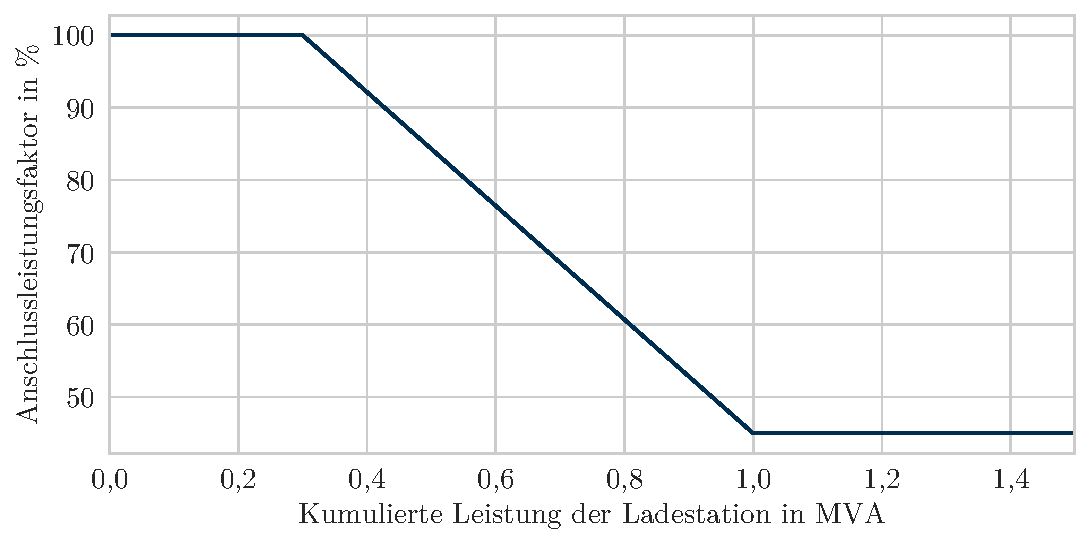
\includegraphics[width=\textwidth]{Bilder/connection_rating_factor}
    \caption{Abhängigkeit des Anschlussleistungsfaktors von der kumulierten Leistung aller Ladepunkte einer Ladestation}\label{fig:connection_rating}
\end{figure}


\subsection{Ladestrategien}\label{chap:theo_strategies}

Innerhalb dieser Arbeit werden zwei präventive Ladestrategien und eine aktive Ladestrategie untersucht.
Auf diese Weise soll analysiert werden, inwieweit eine aktive Ladestrategie gegenüber präventiven Ladestrategien Vorteile aufweist.
Da für aktive Ladestrategien der Aufwand im Betrieb höher ist und zusätzliche Technik benötigt wird, liegen die Kosten für solche Ladestrategien deutlich höher.\medskip

Das Ziel der Ladestrategien ist es, ein möglichst netzfreundliches Verhalten der Ladevorgänge zu erzeugen, ohne den Komfort für Endverbraucher$^*$innen einzuschränken.
Deshalb gilt als Randbedingung aller Ladestrategien, dass der Ladebedarf jedes Ladevorgangs zu \SI{100}{\percent} gedeckt werden muss.
Dies bedeutet, dass Ladevorgänge nur dann flexibilisiert werden können, wenn innerhalb der Standzeit eine Vollladung des \gls{EPKW} möglich ist.
Weiterhin können nur private Ladevorgänge flexibilisiert werden, da bei öffentlichen Ladevorgängen die Erfüllung der Dienstleistung im Vordergrund steht.
Um die drei Ladestrategien bewerten zu können, wird zusätzlich eine Referenz-Ladestrategie untersucht.


\subsubsection{Referenz-Laden}

Bei der Referenz-Ladestrategie wird für Ladevorgänge in der \gls{NS}-Ebene ein vollkommen ungesteuertes Laden der \glspl{EPKW} angenommen.
Da bei großen privaten Ladeparks ein ungesteuertes Laden als unrealistisch einzuschätzen ist, wird davon ausgegangen, dass ab einem Anschluss in der \gls{MS}-Ebene der Betreiber eine Reduktion der Spitzenlast anstrebt.
In diesen Fällen kommt auch bei der Referenz-Ladestrategie das reduzierte Laden zum Einsatz, welches anschließend erläutert wird.


\subsubsection{Ladegruppen}

Das Ziel der Ladegruppen ist es, die Netzbelastung präventiv durch die Senkung der Gleichzeitigkeit der Ladevorgänge zu reduzieren.
Hierfür werden die einzelnen Ladepunkte in zwei Gruppen eingeteilt.
Beiden Gruppen werden alternierend 15-minütige Ladezeitfenster zugewiesen, in denen bei voller Ladeleistung der Ladebedarf gedeckt wird.
Reichen die zugewiesenen Ladezeitfenster nicht aus, um den Ladebedarf des Ladevorgangs zu decken, werden auch die Ladezeitfenster der anderen Gruppe verwendet, bis der Ladebedarf gedeckt werden kann.
Die Ladezeitfenster der eigenen Gruppe werden dabei priorisiert behandelt.
Es wird darauf geachtet, dass die Zuweisung der Gruppen nicht nur innerhalb eines \gls{MS}-Netzgebietes möglichst leistungshomogen erfolgt, sondern detailliert bis in die einzelnen Stränge der \gls{NS}-Ebene.
Innerhalb eines \gls{NS}-Stranges wird weiterhin darauf geachtet, dass auch die einzelnen Leistungsklassen der Ladeinfrastruktur gleichmäßig auf die Gruppen verteilt werden.
Erfolgt der Anschluss einer Ladestation auf der \gls{MS}-Ebene, wird diese Ladestation wie ein eigener \gls{NS}-Strang behandelt und die einzelnen Ladepunkte dementsprechend in die Gruppen eingeteilt.
In \autoref{fig:group_vis} wird beispielhafte die Einteilung von Ladepunkten auf die zwei Gruppen innerhalb eines \gls{NS}-Stranges dargestellt. \cite{Schachler2021}

\begin{figure}[H]
    \centering
    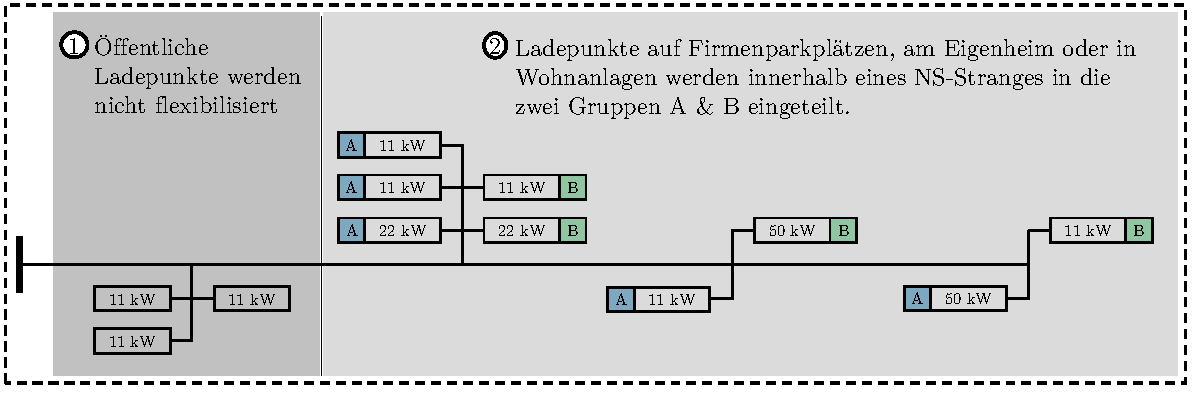
\includegraphics[width=\textwidth]{Bilder/grouped_charging_vis_cropped}
    \caption{Einteilung der Ladepunkte eines NS-Stranges in die Gruppen A und B für das gruppierte Laden}\label{fig:group_vis}
\end{figure}


\subsubsection{Reduziertes Laden}

Im Gegensatz zu den Ladegruppen soll beim reduzierten Laden die Senkung der Netzbelastung präventiv durch die Reduzierung der Ladeleistung der einzelnen Ladevorgänge erreicht werden.
Hierbei wird durch eine Absenkung der Ladeleistung möglichst die gesamte Standzeit des \gls{EPKW} für den Ladevorgang genutzt.
Die Flexibilität dieser Ladestrategie wird durch eine Mindestladeleistung von \SI{10}{\percent} der Nennleistung des angefahrenen Ladepunktes technisch begrenzt.
Hierdurch soll ein Kompromiss zwischen einer möglichst großen Reduktion der Ladeleistung und den technischen Anforderungen der Ladeinfrastruktur gefunden werden.
Im Gegensatz zur Referenz-Ladestrategie werden unabhängig von der Netzebene beim reduzierten Laden alle privaten Ladevorgänge flexibilisiert. \cite{Schachler2021}


\subsubsection{Residuallast-Laden}

Bei dem Residuallast-Laden handelt es sich um eine aktive Ladestrategie, welche an das gesteuerte Laden der Agora Studie \textit{Verteilnetzausbau für die Energiewende} \cite{Agora2019} angelehnt ist.
Der Ladevorgang eines \gls{EPKW} findet hierbei immer innerhalb der Zeitpunkte der Standzeit statt, welche die geringste Residuallast innerhalb des \gls{MS}-Netzgebietes aufweisen, wodurch eine Glättung der Residuallast erreicht werden soll.
Die Zuweisung findet auf Viertelstundenbasis und die Ladevorgänge immer bei voller Ladeleistung statt.
Das Ziel der Optimierung kann so formuliert werden, dass eine Minimierung der \glspl{MQA} nach \autoref{eq:residual} der Residuallast vom Mittelwert der Residuallast angestrebt wird.

\begin{equation}
	\text{MQA} = \frac{1}{n} \sum_i^n \left( P_{\text{R}_i} - \overline{P}_{\text{R}} \right)^2
	\label{eq:residual}
\end{equation}

\noindent Wobei:

\addvbuffer[12pt 12pt]{
	\begin{tabular}{>{$}r<{$}@{\ :\ }l}
		P_{\text{R}_i}				& Residuallast zum Zeitschritt $i$  \\
		\overline{P}_{\text{R}}		& Mittelwert der Residuallast 		\\
		n							& Anzahl an Zeitschritten			\\
		i							& Index des Zeitschrittes 			\\
	\end{tabular}
}

Durch die Abhängigkeit der Residuallast von den einzelnen Ladevorgängen sind auch die Ergebnisse der Optimierung der einzelnen Ladevorgänge voneinander abhängig.
Hierdurch entsteht ein komplexes Optimierungsproblem.
Um die Rechenzeit in einem akzeptablen Maß zu halten, wird eine Näherung an eine optimale Lösung angestrebt.
Für jeden Ladevorgang wird ermittelt, wie viel überschüssige Standzeit zur Flexibilisierung der Ladevorgänge zur Verfügung steht.
Die Ladevorgänge werden anschließend in Abhängigkeit dieses Kriteriums in aufsteigender Reihenfolge sortiert und einzeln betrachtet.
So werden für jeden Ladevorgang die nötigen Zeitschritte für den Ladevorgang ausgewählt, welche innerhalb der Standzeit die geringste Residuallast aufweisen.
Zusätzlich wird die Residuallast entsprechend angepasst und somit die Abhängigkeit der einzelnen Ladevorgänge voneinander gewährleistet.
Auf diese Weise werden Ladevorgänge mit einem geringen Flexibilitätsband vorrangig behandelt und eine möglichst optimale Lösung bei einem geringen Rechenaufwand erreicht.


\subsection{Überführung der Fahrtprofile in Lastzeitreihen}

Die Fahrtprofile der \gls{EPKW} und die Lastzeitreihen der Ladestrategien werden auf \SI{15}{\Minuten} Basis generiert.
In vielen Zeitschritten kann der {--} verbleibende {--} Ladebedarf in weniger als \SI{15}{\Minuten} nachgeladen werden.
Aus diesem Grund wird durch zwei Maßnahmen ein Kompromiss angestrebt, um sowohl realistische Gleichzeitigkeiten abzubilden, die Auswikungen auf die Netzbelastung haben, als auch die Differenz zwischen dem Ladebedarf der Fahrtprofile nach \gls{SIMBEV} und den Lastzeitreihen der Ladestrategien minimal zu halten.

\begin{enumerate}
	\item Dem Gesamtladebedarf eines Ladevorgangs wird nur dann der Ladebedarf des letzten Zeitschritts zugeordnet, wenn bei maximaler Ladeleistung mindestens \SI{20}{\percent} des Zeitschritts benötigt werden, um den Ladebedarf zu decken.
	\item Wenn einem Ladevorgang der Ladebedarf des letzten Zeitschritts zugeordnet wird, dann wird dies in den Lastzeitreihen in allen für die Ladung auch nur anteilig benötigten Zeitschritten durch die zugewiesene Ladeleistung widergespiegelt.
\end{enumerate}

Wenn ein Ladevorgang von diesen Maßnahmen betroffen ist, dann wird der Ladebedarf dieses Ladevorgangs entweder erhöht oder reduziert in den Lastzeitreihen wiedergegeben.
Bei dem reduzierten Laden entsteht diese Problematik bei den flexibilisierbaren Ladevorgängen nicht, da sich die Ladeleistung flexibel nach dem gegebenen Ladebedarf und der zur Verfügung stehenden Standzeit ausrichten kann.
Hierdurch entsteht jedoch eine Differenz in dem Gesamtenergiebedarf der Lastzeitreihen zwischen dem reduzierten Laden und den sonstigen Ladestrategien.
Um dies zu vermeiden werden die zuvor beschriebenen Maßnahmen vor der Erstellung der Lastzeitreihen durchgeführt und der Ladebedarf bereits in den Fahrtprofilen nach \gls{SIMBEV} angepasst.
Auf diese Weise wird sichergestellt, dass sich der Gesamtenergiebedarf der Lastzeitreihen zwischen den Ladestrategien nicht unterscheidet.
Dies soll kurz an zwei Beispielen veranschaulicht werden:

\begin{enumerate}
	\item Beträgt der Ladebedarf eines Fahrzeuges nach \gls{SIMBEV} beispielsweise \SI{12}{\kwh} und die fahrzeugseitige Wirkleistung \SI{9.9}{\kw}, dann werden insgesamt rund \SI{73}{\Minuten} für die Ladung benötigt. In diesem Fall wird in den Lastzeitreihen insgesamt fünf Zeitschritten und somit \SI{75}{\Minuten} die Ladeleistung zugeordnet. Aus diesem Grund wird der Ladebedarf des Ladevorgangs in den Fahrtprofilen nach \gls{SIMBEV} auf \SI{12.375}{\kwh} erhöht.
	\item Wenn hingegen der Ladebedarf bei einer gleichbleibenden Ladeleistung \SI{10}{\kwh} beträgt, dann werden nur rund \SI{61}{\Minuten} für die Ladung benötigt. In diesem Fall wird die Ladeleistung in den Lastzeitreihen nur in vier Zeitschritten und somit \SI{60}{\Minuten} abgebildet. Der Ladebedarf des Ladevorgangs in den Fahrtprofilen nach \gls{SIMBEV} wird entsprechend auf \SI{9.9}{\kwh} reduziert.
\end{enumerate}


\subsection{Netzuntersuchung}\label{chap:edisgo_theo}

Das Open Source Tool \gls{EDISGO} stellt eine Toolbox zur Verfügung, um Verteilnetze auf Netzprobleme zu untersuchen.
Gleichzeitig können mit \gls{EDISGO} Maßnahmen zur Behebung der Netzprobleme bewertet werden.
Dabei bilden synthetische Netztopologien, die mit Hilfe des Open Source Tools \gls{DINGO} erzeugt wurden, die Grundlage für die Berechnungen mit \gls{EDISGO}.
\gls{EDISGO} kann über \textit{GitHub} \cite{edisgoGit2019} abgerufen werden und ist auf \textit{Read the Docs} \cite{edisgoDocs2017} dokumentiert.
Innerhalb dieses Kapitels werden die wichtigsten Funktionalitäten \glspl{EDISGO} für die Durchführung der Berechnungen innerhalb dieser Arbeit dargestellt und erläutert.


\subsubsection{Ermittlung von Netzproblemen}\label{chap:grid_issues}

Die Überprüfung der einzelnen Netze auf Netzprobleme erfolgt in zwei Schritten.
Vorerst wird eine nichtlineare Lastflussanalyse durchgeführt, um anschließend die Einhaltung der Spannungsanforderungen und technischen Richtlinien bezüglich der Betriebsmittelbelastungen zu überprüfen.
Die Durchführung der Lastflussanalyse erfolgt mit Hilfe des Open Source Tools \textit{PyPSA} \cite{Brown2020}.
In diesem Kapitel soll auf die theoretischen Grundlagen der Lastflussanalyse, den Umfang der Analyse und die Spannungsanforderungen sowie die technischen Richtlinien bezüglich der Gerätebelastungen eingegangen werden.\medskip

Das Ziel der Lastflussanalyse ist es, dass zwischen allen Verbindungen der Netzknoten $i$ und $k$ die folgende Gleichung erfüllt wird:

\begin{equation}
	S_i = P_i + j Q_i = V_i I_i^* = V_i \left(\sum_j Y_{i,k} V_k \right)^*
	\label{eq:pf}
\end{equation}

\noindent Wobei:

\addvbuffer[12pt 12pt]{
	\begin{tabular}{>{$}r<{$}@{\ :\ }l}
		S_i 		& Scheinleistung am Netzknoten $i$ \\
		P_i	 		& Wirkleistung am Netzknoten $i$ \\
		Q_i			& Blindleistung am Netzknoten $i$ \\
		V_i			& Komplexe Spannung am Netzknoten, wobei $V_i = \left| V_i \right|e^{j \theta_i}$ \\
		I_i			& Stromstärke am Netzknoten \\
		Y_{i,k}		& Admittanz der Leitung zwischen den Netzknoten $i$ und $k$ \\
	\end{tabular}
}

Der Winkel der komplexen Spannung ist relativ zum Bilanzknoten.
Unter dem Bilanzknoten wird ein Netzknoten verstanden, an welchem der Wirk- und Blindleistungsfluss frei eingestellt werden kann.
Mit Hilfe des Bilanzknotens kann über einen iterativen Prozess die Konvergenz nach \autoref{eq:pf} des Systems erreicht werden.
Eine genau Beschreibung der Lastflussanalyse des Open Source Tools \textit{PyPSA} kann auf \textit{Read the Docs} \cite{Brown2020a} abgerufen werden.
Da die Spannung der Sekundärseite des \gls{HS}-\gls{MS}-\glspl{USW} eingestellt werden kann, eignet sich dieser Punkt besonders gut und wird entsprechend als Bilanzknoten verwendet.
Alle weiteren Netzknoten werden mit gegebenen Wirk- und Blindleistungen modelliert. \cite{Schachler}\medskip

Die Lastflussanalyse der Netze berücksichtigt sowohl \gls{MS}- und \gls{NS}-Leitungen als auch die \gls{MS}-\gls{NS}-Umspannebene.
Gegenüber einer Aggregation der Erzeugung und des Bedarfs der einzelnen \gls{NS}-Netze an dem jeweiligen \gls{MS}-\gls{NS}-\gls{USW} bietet diese besonders tiefgehende Betrachtung die Möglichkeit, die Auswirkungen der teilweise hohen Ladeleistungen der Ladeinfrastruktur genauer zu betrachten und den Einfluss verschiedener Ladestrategien umfassender bestimmen zu können.
Da die Sekundärseite des \gls{HS}-\gls{MS}-\glspl{USW} als Bilanzknoten modelliert wird, können an dieser keine Spannungsprobleme auftreten.
Jedoch entspricht die Scheinleistung des Bilanzknotens der Lastflussanalyse der Leistung, die über das \gls{HS}-\gls{MS}-\gls{USW} geleitet wird.
Anhand dieses Wertes können zusätzlich Aussagen über die Belastung des \gls{HS}-\gls{MS}-\glspl{USW} getroffen werden.
In \autoref{fig:scope} ist eine Übersicht über den Umfang der Lastflussanalyse dargestellt. \cite{Schachler}

\begin{figure}[H]
    \centering
    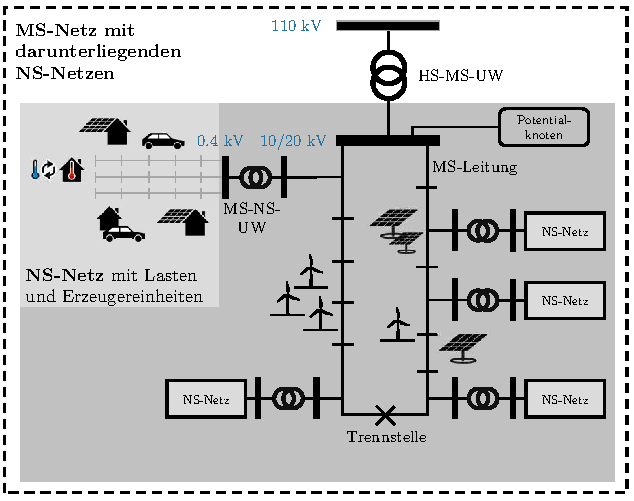
\includegraphics[width=\textwidth]{Bilder/scope_power_flow_kh_cropped}
    \caption[Umfang der Lastflussanalyse mit eDisGo]{Umfang der Lastflussanalyse mit eDisGo \cite{Schachler}}\label{fig:scope}
\end{figure}

Mit Hilfe der durch die Lastflussanalyse ermittelten Belastungen und Spannungsabweichungen an den Betriebsmitteln können abschließend Überlastungen und Spannungsprobleme festgestellt werden.
Im Rahmen dieser Arbeit gilt als Planungsgrundsatz, dass der zulässige Belastungsfaktor aller Betriebsmittel \SI{100}{\percent} beträgt.
Die zulässigen Spannungsabweichungen liegen für Endkunden in der \gls{NS}-Ebene bei \SI{\pm 10}{\percent}.
Dieses Spannungsband wird nach \autoref{tab:Spannungsband} auf die \gls{MS}, \gls{MS}-\gls{NS}- und \gls{NS}-Ebene aufgeteilt.
Im Lastfall spiegelt das in der \gls{NS}-Ebene größere zulässige Spannungsband wider, dass in dieser Ebene die Mehrzahl der Verbraucher angeschlossen ist.
Demgegenüber wird im Rückspeisefall ein größeres Spannungsband für die \gls{MS}-Ebene reserviert.
Es gelten die in \autoref{tab:Spannungsband} Spannungsabweichungen, welche aus \textit{Integrated Techno-Economic Power System Planning of Transmission and Distribution Grids} \cite{Mueller2019a} entnommen wurden und auf der \textit{Verteilnetzstudie für das Land Baden-Württemberg} \cite{Rehtanz2017} basieren.

{
\renewcommand{\arraystretch}{1.2}% grßerer Zeilenabstand
\sisetup{range-phrase=~bis~}
\begin{table}[H]
	\begin{center}
		\caption{Zulässige Spannungsabweichungen der Betriebsmittel in der MS- und NS-Ebene}
		\begin{tabu} to 0.5\textwidth {X[1.2] X[1, r] X[1, r]}
			\toprule
			Spannungsebene & Lastfall               & Rückspeisefall             \\ \midrule
			MS             & \SI{-1.5}{\percent}    & \SI[retain-explicit-plus]{+5.0}{\percent}   	 \\
			MS-NS          & \SI{-2.0}{\percent}    & \SI[retain-explicit-plus]{+1.5}{\percent}   	 \\
			NS             & \SI{-6.5}{\percent}    & \SI[retain-explicit-plus]{+3.5}{\percent}   	 \\ \bottomrule
            \multicolumn{3}{l}{Quelle: \cite{Rehtanz2017}}
		\end{tabu}
		\label{tab:Spannungsband}
	\end{center}
	\vspace{-3mm}%Put here to reduce too much white space after your table
\end{table}
}


\subsubsection{Ermittlung des Abregelungsbedarfs für die Auflösung von Netzüberlastungen}

Die Ermittlung des Abregelungsbedarfs für die Auflösung von Spannungsbandverletzungen und Betriebsmittelüberbelastungen erfolgt in einem iterativen Prozess.
Vorerst werden etwaige Netzprobleme und die entsprechenden Zeitschritte, in denen die Netzprobleme auftreten, mit Hilfe der zuvor beschriebenen Lastflussanalyse ermittelt.
Anschließend wird die Last bzw. die Einspeisung in \SI{5}{\percent}-Schritten innerhalb der ermittelten Zeitschritte reduziert.
Beides wird so lange wiederholt, bis keine Netzprobleme mehr auftreten.\medskip

Um die Rechenzeit innerhalb eines akzeptablen Maßes zu halten, erfolgt die Ermittlung des Abregelungsbedarfs für zwei Wochen des Jahres.
Hierbei werden die Wochen untersucht, die im \gls{MS}-Netzgebiet die minimale bzw. maximale durchschnittliche Residuallast aufweisen.
Auf diese Weise sollen möglichst extreme Belastungssituationen abgedeckt werden.\medskip

Aufgrund der hohen Anzahl an \glspl{EPKW}, \glspl{WP} und erneuerbaren Erzeugereinheiten kommt es in einigen Fällen dazu, dass die Lastflussanalyse nicht konvergiert.
Aus diesem Grund werden zuerst die \gls{NS}-Netze eines \gls{MS}-Netzgebiets einzeln betrachtet, um dort extreme Belastungssituationen abzufangen, die eine Konvergenz des Gesamtsystems verhindern können.\medskip
% Durch die vorgeschaltete Einzelbetrachtung der \gls{NS}-Netze kann der Abregelungsbedarf eindeutig der \gls{NS}- bzw. \gls{MS}-Ebene zugeordnet werden.\medskip

Bei der Lösung der Netzprobleme werden vorerst Spannungsprobleme und abschließend Überlastungen behandelt.
Weiterhin werden Probleme in der \gls{NS}-Ebene behandelt, bevor Probleme in der \gls{MS}-\gls{NS}-Umspannebene und abschließend in der \gls{MS}-Ebene gelöst werden.
Durch die Auflösung von Netzproblemen auf tieferen Spannungsebenen können unter Umständen bereits Netzprobleme in darüber liegenden Spannungsebenen gelöst, entspannt oder auch verstärkt werden.
Weiterhin werden Netzprobleme innerhalb der \gls{NS}- bzw. \gls{MS}-Ebene anhand ihrer Entfernung zur übergeordneten Umspannebene priorisiert.
So kann auch hier die Lösung von weiter entfernten Netzproblemen bereits vorgeschaltete Netzprobleme auflösen oder entspannen.
Für jeden Zeitschritt, in dem Überlastungs- oder Spannungsprobleme an einem Netzknoten auftreten, wird geprüft, ob die Netzprobleme durch hohe Nachfrage oder hohe Einspeisung entstehen.
Anhand dieser Information wird entschieden, ob Last oder Einspeisung abgeregelt werden soll.
Die gesamte notwendige Abregelung für das \gls{MS}-Netzgebiet ergibt sich aus der Summierung aller nötigen Abregelungen von Last und Erzeugung.
In \autoref{fig:scope_curtailment} ist das Vorgehen veranschaulicht.

\begin{figure}[H]
    \centering
    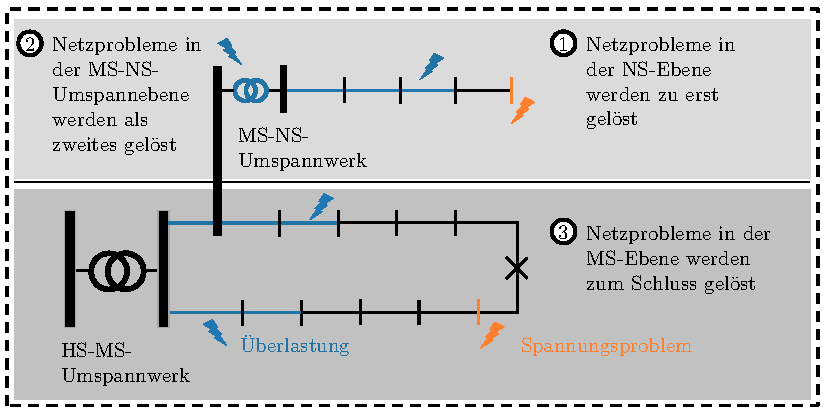
\includegraphics[width=\textwidth]{Bilder/grid_issues_scope_cropped}
    \caption[Umfang der Ermittlung des Abregelungsbedarfs für die Auflösung von Spannungsbandverletzungen und Betriebsmittelüberbelastungen]{Umfang der Ermittlung des Abregelungsbedarfs für die Auflösung von Netzüberlastungen \cite{Schachler}}\label{fig:scope_curtailment}
\end{figure}


\clearpage



\section{Szenariorahmen}\label{chap:Szenariorahmen}

Innerhalb des Workshops \glqq Neue Verbraucher und elektrische Flexbilitäten\grqq{} wurden Fragestellungen diskutiert, die sich mit der Integration neuer Verbraucher und der Nutzung elektrischer Flexibilitäten in Übertragungs- und Verteilnetzen befassen \cite{RLI2020}.
Hierbei wurden unter anderem die Ergebnisse der Metaanalyse (s. \autoref{chap:Literatur}) genutzt, um mit Branchenexpertinnen und -experten Forschungsfragen zu entwerfen und zukünftige Entwicklungen abzuwiegen.
Die wichtigsten Ergebnisse des Workshops werden kurz vorgestellt und dienen als Leitlinien für die Erstellung eines geeigneten Szenariorahmens für diese Arbeit innerhalb diesen Kapitels.


\subsection{Ergebnisse des Workshops \glqq Neue Verbraucher und elektrische Flexbilitäten\grqq{}}

In diesem Kapitel werden die für diese Arbeit wichtigsten Ergebnisse des Workshops \glqq Neue Verbraucher und elektrische Flexbilitäten\grqq{} aufgelistet.
Zu den Teilnehmern$^*$innen des Workshops zählten mehrheitlich Mitarbeiter$^*$innen von Netzbetreibern, Forschungsinstituten und energiewirtschaftlichen Unternehmen.
Die folgende Auflistung entspricht den relevantesten Ergebnissen mehrerer Diskussionen und Umfragen innerhalb des Workshops.

\begin{itemize}
%	\item Die Untersuchung eines Mobilitätswende-Szenarios ist von besonders hohem Interesse
	\item Private Ladeinfrastruktur zu Hause oder an Firmenparkplätzen besitzt die größte Attraktivität für Verbraucher
%	\item Es wird davon ausgegangen, dass \num{2050} etwa \num{15} \glspl{EPKW} auf einen öffentlichen Ladepunkt kommen
	\item Eine regionale Konzentration von \glspl{EPKW} wird nur während der Markthochlaufphase eine relevante Rolle spielen
	\item Marktorientierte Ladestrategien können Gleichzeitigkeiten und damit den Netzausbaubedarf erhöhen
	\item Die Umsetzung von \gls{V2G}-Anwendungen wird als unwahrscheinlich eingestuft
	
\end{itemize}


\subsection{Szenarien}

In diesem Kapitel erfolgt eine Beschreibung der Annahmen zu den untersuchten Szenarien und somit den Eingangsparametern für die Simulation des Einflusses der Netzintegration von \gls{EPKW}.
Hierzu zählen der Ausbau regenerativer Energien, der konventionelle Stromverbrauch, der Hochlauf von \glspl{WP} und \glspl{EPKW} sowie deren technische Parameter.
Der Fokus liegt hierbei auf der Aufstellung von Annahmen zum Hochlauf von \glspl{EPKW} und zur Verfügbarkeit der Ladeinfrastruktur.
Insgesamt werden drei Szenarien und eine daraus abgeleitete Sensitivität in Form einer Szenarette untersucht.


\subsubsection{Ausbau regenerativer Energien}

Die Annahmen zu dem Hochlauf der regenerativen Erzeugerkapazitäten werden über die Szenarien hinweg als konstant angenommen.
Hierdurch werden Vermischungseffekte durch die Änderung mehrerer Eingangsparameter verhindert und der Einfluss der Elektromobilität kann getrennt betrachtet werden.
Die Annahmen zum Hochlauf der Erzeugerkapazitäten werden aus dem Szenario \ego des \gls{OPENEGO} Projekts \cite{Mueller2019} entnommen.
Die Regionalisierung der Erzeugerkapazitäten erfolgte im Rahmen des \gls{OPENEGO} Projektes und ist nicht Teil dieser Arbeit.
An dieser Stelle erfolgt eine zusammenfassende Beschreibung der Methodik.
Eine genaue Beschreibung der Regionalisierung findet sich im \gls{OPENEGO} Projektabschlussbericht.\medskip

Um den Status Quo abzubilden, werden offizielle, öffentliche Verzeichnisse, welche Informationen zu den einzelnen Kraftwerken bereitstellen zusammengeführt.
Da die Daten hierbei in unterschiedlichen Qualitäten und Detailgraden vorliegen, müssen diese auf ein einheitliches Format ergänzt werden.
Ziel ist es dabei allen Anlagen einen geografischen Bezugspunkt, sowie eine Netzebene zuzuordnen.
Je nach Datensatz werden hierbei die angegebene Spannungsebene, die eingetragene Technologie und die installierte Leistung der Kraftwerke als Identifikator genutzt.\medskip

Für das Szenario \ego werden die Hochlaufzahlen für regenerative Erzeugerkapazitäten aus der Studie \textit{e-Highway 2050 - Modular Development Plan of the Pan-European Transmission System 2050} \cite{EEHPG2015} übernommen, welche sich in \autoref{tab:EE-RampUp} finden.
Auf Grundlage des zuvor erstellten Status Quo werden die Erzeugerkapazitäten entsprechend der aktuellen Verteilung gewichtet verteilt.
Hierbei werden maximale Ausbaupotentiale berücksichtigt, indem beispielsweise Weißflächen für den Ausbau von Onshore Windkraftanlagen berücksichtigt werden.

{
\renewcommand{\arraystretch}{1.2}% grßerer Zeilenabstand
\sisetup{range-phrase=~{--}~}% Gedankenstrich statt "bis" bei SIrange
\begin{table}[H]
	\begin{center}
		\caption{Hochlaufzahlen der regenerativen Erzeugerkapazitäten}
		\begin{tabu} to 0.45\textwidth {X[1] X[1.5, r]}
			\toprule
			              & Erzeugerkapazitäten \\ \midrule
			Wind Onshore  & \SI{98.4}{\gw}                      \\
			Wind Offshore & \SI{27.0}{\gw}                      \\
			Photovoltaik  & \SI{97.8}{\gw}                      \\
			Biomasse      & \SI{27.8}{\gw}                      \\
			Wasserkraft   & \SI{3.2}{\gw}                       \\ \bottomrule
		\end{tabu}
		\label{tab:EE-RampUp}
	\end{center}
	\vspace{-3mm}%Put here to reduce too much white space after your table
\end{table}
}

Die Zeitreihen für die Erzeugung aus Wind- und \gls{PV}-Anlagen werden der \gls{OEP} \cite{OEP} entnommen und sind frei verfügbar.
Im Falle der Energieerzeugung aus Biomasse und Wasserkraft wird eine konstante Erzeugung angenommen.
So waren in Deutschland im Jahr \num{2019} \SI{9983}{\mw} an Biomasse- und \SI{5595}{\mw} an Wasserkraftwerken installiert die insgesamt \SI{50009}{\gwh} und \SI{20058}{\gwh} Energie erzeugten \cite{BMWi2020}.
Der hieraus resultierende Leistungsfaktor von \num{0.57} und \num{0.41} wird auf alle Biomasse- und Wasserkraft-Erzeugerkapazitäten unverändert umgelegt.
In den untersuchten Netzgebieten finden sich keine konventionellen Kraftwerke.


\subsubsection{Konventioneller Stromverbrauch}

Bei dem konventionellen Stromverbrauch handelt es sich um geographisch hochaufgelöste Zeitreihen, die jeweils einem sogenannten \Lastgebiet zugeordnet werden.
Der konventionelle Stromverbrauch entstammt parallel zum Ausbau der regenerativen Energien aus dem \gls{OPENEGO} Projekt und wurde im entsprechenden Projektbericht \cite{Mueller2019} ausführlich beschrieben.
An dieser Stelle soll die Methodik kurz zusammengefasst werden.\medskip

Die \Lastgebiete entsprechen einer geographischen Einheit, der ein elektrischer Verbrauch zugeordnet wird.
Um die Datenmengen möglichst gering zu halten, werden innerhalb eines \Lastgebietes räumlich nahe liegende Landnutzungsflächen zusammengefasst.
Zusätzlich wird den \Lastgebieten eine Bevölkerungsanzahl und der Anteil an den Gesamtlandnutzungsflächen (\gls{GHD}, Industrie, Wohnen und Landwirtschaft) zugeordnet.
Anhand dieser Charakteristiken erfolgt abschließend eine anteilige Zuordnung des Stromverbrauches und der Zeitreihen der vier Sektoren auf die \Lastgebietedot.


\subsubsection{Wärmepumpen}

Der Hochlauf an \glspl{WP} in Deutschland wird über die Szenarien hinweg als feste Eingangsgröße angenommen.
Die Hochlaufzahlen und der Jahresverbrauch entsprechen dem Szenario C~\num{2035} des \glspl{NEP} \numrange[range-phrase=~{--}~]{2021}{2035} \cite{BNetzA2020} und finden sich in \autoref{tab:WP-RampUp}.

{
\renewcommand{\arraystretch}{1.2}% grßerer Zeilenabstand
\sisetup{range-phrase=~{--}~}% Gedankenstrich statt "bis" bei SIrange
\begin{table}[H]
	\begin{center}
		\caption{Hochlaufzahlen für Wärmepumpen}
		\begin{tabu} to 0.6\textwidth {X[1.5] X[1, r]}
			\hline
										 & Wärmepumpen \\ \hline
			Anzahl in \si{\MioStkSC}     & \num{7.0}   \\
			Leistung in \si{\gw}         & \num{21.0}  \\
			Jahresverbrauch in \si{\twh} & \num{22.4}  \\ \hline
		\end{tabu}
		\label{tab:WP-RampUp}
	\end{center}
	\vspace{-3mm}%Put here to reduce too much white space after your table
\end{table}
}

Der Jahresstromverbrauch der \glspl{WP} wird anhand des Anteils des Stromverbrauches des Haushaltssektors eines Netzgebietes bezogen auf den Gesamtstromverbrauch des Haushaltssektors im Szenario \ego auf die einzelnen Netzgebiete verteilt.
Innerhalb eines Netzgebietes erfolgt die Regionalisierung gewichtet anhand des Stromverbrauches der einzelnen Haushaltslasten.
Die zeitliche Verteilung der Last wird der nichtöffentlichen Studie \textit{E-Mobility Study {--} Assessment of coordinated charging considering distribution grid restrictions} \cite{Schachler} entnommen.


\subsubsection{Elektromobilität}\label{chap:EMob_Szenarien}

Bei der Elektromobilität müssen neben Annahmen zu den Zahlen zum Fahrzeughochlauf auch die technischen Daten der Fahrzeuge und die Verfügbarkeit der Ladeinfrastruktur berücksichtigt werden.


\paragraph{Fahrzeughochlauf:}
Der Fahrzeughochlauf unterscheidet sich je nach Szenario.
Insgesamt spiegeln alle Szenarien unterschiedlich starke Durchdringungen des \glspl{MIV} mit \gls{EPKW} wider.\medskip

Das erste Szenario entspricht mit einem Fahrzeughochlauf von \SI{14}{\MioStk} den Annahmen des Szenarios C~\num{2035} des \gls{NEP} \numrange[range-phrase=~{--}~]{2021}{2035} \cite{BNetzA2020}.
Die Hochlaufzahlen für das Referenzszenario entsprechen mit \SI{25.1}{\MioStk} den summierten Medianen der Literaturrecherche für den Fahrzeughochlauf an \glspl{BEV} und \glspl{PHEV} im Jahr \num{2050}.
% Beim Mobilitätswende-Szenario wurde der Fahrzeugbestand des Effizienz-Plus Szenarios des Renewbility~III Projekts \cite{Institut2016} übernommen und von einer vollständigen Elektrifizierung ausgegangen.
Das Antriebswende-Szenario geht hingegen von einer vollständigen Elektrifizierung des Fahrzeugbestandes von \SI{47.7}{\MioStk} vom \DTMdate{2020-01-01} \cite{KBA2020} aus.

{
\renewcommand{\arraystretch}{1.2}% grßerer Zeilenabstand
\sisetup{range-phrase=~{--}~}% Gedankenstrich statt "bis" bei SIrange
\begin{table}[H]
	\begin{center}
		\caption{E-Pkw Hochlaufzahlen je Szenario}
		\begin{tabu} to 0.6\textwidth {X[1] X[2, r]}
			\hline
			Szenario         & E-PKW in \si{\MioStk}	\\ \hline
			NEP C~\num{2035} & \num{14.0}               \\
			Referenz         & \num{25.1}               \\
			Mobilitätswende  & \num{37.7}               \\
			Antriebswende    & \num{47.7}               \\ \hline
		\end{tabu}
		\label{tab:SzenarienRampUp}
	\end{center}
	\vspace{-3mm}%Put here to reduce too much white space after your table
\end{table}
}

Die Aufteilung des Fahrzeugbestandes in \glspl{BEV} und \glspl{PHEV} erfolgt anhand des ermittelten Medians der Literaturrecherche für den Fahrzeughochlauf an \glspl{BEV} und \glspl{PHEV} für das Stützjahr \num{2050}.
Innerhalb der Fahrzeugtypen erfolgt weiterhin eine Einteilung in die Fahrzeugklassen Kleinwagen, Mittelklasse und Oberklasse.
Es wird davon ausgegangen, dass sich die Einteilung in Fahrzeugklassen zwischen \glspl{BEV} und \glspl{PHEV} nicht unterscheidet.
So gibt es in den Szenarien zwar insgesamt mehr \glspl{BEV} als \glspl{PHEV}, aber das Verhältnis zwischen den Fahrzeugklassen ist zwischen den beiden Fahrzeugtypen konstant.
Die Einteilung in \autoref{tab:CarSplit} entspricht der Statistik des Kraftfahrt-Bundesamtes \cite{KBASegments2020} vom \DTMdate{2020-01-01}.
Es wird somit von einer Fortschreibung des aktuellen Verbraucherverhaltens ausgegangen.
Eine genaue Zuordnung der \gls{PKW}-Segmente in die Klassen findet sich im Anhang in \autoref{tab:KBASegments} und \autoref{tab:Segments}.

{
\renewcommand{\arraystretch}{1.2}% grßerer Zeilenabstand
\sisetup{range-phrase=~{--}~}% Gedankenstrich statt "bis" bei SIrange
\begin{table}[H]
	\begin{center}
		\caption{Aufteilung der E-Pkw auf die einzelnen Fahrzeugtypen und -klassen}
		\begin{tabu} to 0.4\textwidth {X[1.5] X[1, r]}
			\toprule
			Fahrzeugklasse    & Anteil  \\ \midrule
			BEV Kleinwagen    & \SI{15.9}{\percent}               \\
			BEV Mittelklasse  & \SI{35.3}{\percent}               \\
			BEV Oberklasse    & \SI{10.5}{\percent}               \\
			PHEV Kleinwagen   & \SI{9.8}{\percent}                \\
			PHEV Mittelklasse & \SI{21.9}{\percent}               \\
			PHEV Oberklasse   & \SI{6.5}{\percent}                \\ \bottomrule
		\end{tabu}
		\label{tab:CarSplit}
	\end{center}
	\vspace{-3mm}%Put here to reduce too much white space after your table
\end{table}
}


\paragraph{Technische Daten:}

Die technischen Daten der Fahrzeuge sind klassenspezifisch und werden innerhalb ihrer Klasse als homogen angenommen.
In \autoref{tab:TechPowerCap} finden sich die fahrzeugseitige maximale Ladeleistung und die nutzbare Batteriekapazität der jeweiligen Fahrzeugklassen.
Die Annahmen wurden dem Szenario \textit{Verstärkte Elektrifizierung} für das Jahr \num{2049} aus der Studie \textit{Automobile Wertschöpfung 2030/2050} \cite{Kaul2019} entnommen.
Eine Limitierung der Ladeleistung durch die Unterscheidung in Normal- und Schnellladung erfolgt im Simulationsmodell von Seiten der Ladeinfrastruktur.

{
\renewcommand{\arraystretch}{1.2}% grßerer Zeilenabstand
\sisetup{range-phrase=~{--}~}% Gedankenstrich statt "bis" bei SIrange
\begin{table}[H]
	\begin{center}
		\caption{Maximale Ladeleistung und nutzbare Batteriekapazität je Fahrzeugklasse}
		\begin{tabu} to \textwidth {X[0.9] X[1.3, r] X[1.5, r]}
				\hline
				Fahrzeugklasse    & Maximale Ladeleistung in \si{\kw} & Nutzbare Batteriekapazität in \si{\kwh} \\ \hline
				BEV Kleinwagen    & \num{120}                         & \num{70}                                \\
				BEV Mittelklasse  & \num{350}                         & \num{100}                               \\
				BEV Oberklasse    & \num{350}                         & \num{120}                               \\
				PHEV Kleinwagen   & \num{120}                         & \num{25}                                \\
				PHEV Mittelklasse & \num{120}                         & \num{30}                                \\
				PHEV Oberklasse   & \num{120}                         & \num{40}                                \\ \hline
            \multicolumn{3}{l}{Quelle: Szenario \textit{Verstärkte Elektrifizierung} für das Jahr \num{2049} \cite{Kaul2019}}
		\end{tabu}
		\label{tab:TechPowerCap}
	\end{center}
	\vspace{-3mm}%Put here to reduce too much white space after your table
\end{table}
}

Der elektrische Energieverbrauch der Fahrzeuge wird aus den Annahmen der Studie \textit{eMobil 2050} \cite{Hacker2014} abgeleitet.
Es wird angenommen, dass Kleinwagen gegenüber Mittelklasse Fahrzeugen einen um \SI{20}{\percent} reduzierten Energieverbrauch aufweisen.
Oberklasse Fahrzeuge weisen hingegen einen um \SI{20}{\percent} erhöhten Energieverbrauch auf.\medskip

Weiterhin bietet die Studie \textit{eMobil 2050} nur Verbrauchsangaben nach dem \glspl{NEFZ}, welche nicht realen Verbrauchsdaten entsprechen.
Nach \textit{Informationen zur Umweltpolitik - 189} \cite{Heinfellner2015} lag der Realverbrauch \num{2013} gegenüber einer Messung nach \gls{NEFZ} im Mittel um \SI{27}{\percent} höher.
Die Werte für das Jahr \num{2050} der Studie \textit{eMobil 2050} werden um diesen Faktor erhöht und die Ergebnisse in \autoref{tab:TechVerbrauch} zusammengefasst.

{
\renewcommand{\arraystretch}{1.2}% grßerer Zeilenabstand
\sisetup{range-phrase=~{--}~}% Gedankenstrich statt "bis" bei SIrange
\begin{table}[H]
	\begin{center}
		\caption{Durchschnittlicher elektrischer Energieverbrauch je Fahrzeugklasse}
		\begin{tabu} to 0.6\textwidth {X[1] X[1.2, r]}
			\toprule
			Fahrzeugklasse    & Verbrauch in \si{\kwhkm} \\ \midrule
			BEV Kleinwagen    & \num{11.9}              \\
			BEV Mittelklasse  & \num{14.8}              \\
			BEV Oberklasse    & \num{17.8}              \\
			PHEV Kleinwagen   & \num{12.1}              \\
			PHEV Mittelklasse & \num{15.2}              \\
			PHEV Oberklasse   & \num{18.2}              \\ \bottomrule
		\end{tabu}
		\label{tab:TechVerbrauch}
	\end{center}
	\vspace{-3mm}%Put here to reduce too much white space after your table
\end{table}
}


\paragraph{Ladeinfrastruktur:}

Die Ladeinfrastruktur wird im Gegensatz zu den Annahmen zum Fahrzeughochlauf nicht in absoluten Zahlen ausgedrückt.
Stattdessen werden den einzelnen Wegezwecken der Fahrzeuge Wahrscheinlichkeiten zugeordnet, dass ein Fahrzeug am Zielort geladen werden kann.
Weiterhin wird diese Wahrscheinlichkeit auf verschiedene Ladeleistungen aufgeteilt.
Dabei wird grundsätzlich zwischen Normal- und Schnellladung unterschieden.


\subparagraph{Normalladung} beinhaltet in dieser Arbeit die Leistungsklassen \SI{3.7}{\kw}, \SI{11}{\kw}, \SI{22}{\kw} und \SI{50}{\kw}.
Um zu bestimmen, mit welcher Ladeleistung an einem Zielort geladen werden kann, werden den unterschiedlichen Wegezwecken nach \glspl{MID} (s. \autoref{chap:MID}) dezidiert Wahrscheinlichkeiten zugeordnet, ob und mit welcher Ladeleistung geladen werden kann.
Eine Zuordnung der Leistungsklassen auf die einzelnen Wegezwecke erfordert vorerst eine Zuordnung der \UCs auf die Wegezwecke.
Unter den \UCs werden die fünf Standortarten Eigenheim, Wohnanlage, Firmenparkplatz, Gewerbeparkplatz und Straßenrand verstanden.
In \autoref{tab:WegLadeUseCase} findet sich die entsprechende prozentuale Aufteilung der \UCs auf die Wegezwecke.

{
\renewcommand{\arraystretch}{1.2}% grßerer Zeilenabstand
\sisetup{range-phrase=~{--}~}% Gedankenstrich statt "bis" bei SIrange
\begin{table}[H]
	\begin{center}
		\caption{Prozentuale Zuordnung der Lade Use cases auf die verschiedenen Wegezwecke}
		\begin{tabu} to \textwidth {X[1.2] X[1.1, r] X[1.3, r] X[1.7, r] X[1.8, r] X[1.2, r]}
			\toprule
			Wegezweck  & Eigenheim         & Wohnanlage        & Firmenparkplatz   & Gewerbeparkplatz  & Straßenrand       \\ \midrule
			Arbeit     & \SI{0}{\percent}  & \SI{0}{\percent}  & \SI{65}{\percent} & \SI{0}{\percent}  & \SI{35}{\percent} \\
			dienstlich & \SI{0}{\percent}  & \SI{0}{\percent}  & \SI{38}{\percent} & \SI{6}{\percent}  & \SI{56}{\percent} \\
			Ausbildung & \SI{0}{\percent}  & \SI{0}{\percent}  & \SI{65}{\percent} & \SI{0}{\percent}  & \SI{35}{\percent} \\
			Einkauf    & \SI{0}{\percent}  & \SI{0}{\percent}  & \SI{0}{\percent}  & \SI{77}{\percent} & \SI{24}{\percent} \\
			Erledigung & \SI{0}{\percent}  & \SI{0}{\percent}  & \SI{0}{\percent}  & \SI{38}{\percent} & \SI{62}{\percent} \\
			Freizeit   & \SI{0}{\percent}  & \SI{0}{\percent}  & \SI{0}{\percent}  & \SI{39}{\percent} & \SI{62}{\percent} \\
			nach Hause & \SI{43}{\percent} & \SI{25}{\percent} & \SI{0}{\percent}  & \SI{0}{\percent}  & \SI{31}{\percent} \\ \bottomrule
		\end{tabu}
		\label{tab:WegLadeUseCase}
	\end{center}
	\vspace{-3mm}%Put here to reduce too much white space after your table
\end{table}
}

Derzeit leben in Deutschland ungefähr \SI{44.2}{\MioMen} in Gebäuden mit maximal zwei Wohnungen und \SI{37.2}{\MioMen} in Mehrfamilienhäusern.
Etwa \SI{80}{\percent} der \linebreak Fahrzeugbesitzer$^*$innen in Gebäuden mit maximal zwei Wohnungen verfügen über einen Stellplatz in der Garage oder unter einem Carport.
In Mehrfamilienhäusern verfügen hingegen nur \SI{55}{\percent} der Fahrzeugbesitzer$^*$innen über einen Stellplatz für ihr Fahrzeug \cite{dena2020}.
Unter der vereinfachenden Annahme einer gleichmäßigen Verteilung von Fahrzeugen zwischen Fahrzeugbesitzern$^*$innen in Ein- und Mehrfamilienhäusern ergibt sich hieraus die ermittelte Aufteilung der \UCs auf den Wegezweck \nHdot.\medskip

Die Aufteilung der \UCs auf die Wegezwecke \Einkaufdot, \Erledigung und \Freizeitdot, ergeben sich aus den Wegeanteilen nach Fahrtzweck im \gls{MIV}-Privatverkehr \cite{Rikus2015}.
Im Falle des Wegezwecks \Einkauf, wird angenommen, dass Lebensmittelgschäfte einen Gewerbeparkplatz für jeden Kunden vorhalten.
Weiterhin wird angenommen, dass im Falle von sonstigen Waren und sonstigen Dienstleistungen in \SI{50}{\percent} der Fälle ein Gewerbeparkplatz zur Verfügung steht.
Bei dem Wegezweck \Erledigung wird davon ausgegangen, dass beim Besuch von Behörden, Banken, Post und Geldautomaten ein Gewerbeparkplatz vorhanden ist und bei sonstigen Erledigungen in \SI{50}{\percent} der Fälle.
Für den Wegezweck \Freizeitdot, wird angenommen, dass bei kulturellen Einrichtungen und Veranstaltungen ein Gewerbeparkplatz vorhanden ist.
Bei sonstigen Freizeitaktivitäten wird angenommen, dass in \SI{50}{\percent} der Fälle ein Gewerbeparkplatz vorhanden ist.
In allen verbleibenden Fällen erfolgt ein Parken am Straßenrand.\medskip

Für die Abschätzung der Wahrscheinlichkeit auf einem Firmenparkplatz für den Wegezweck \Arbeit parken zu können, wurde die Parkplatzsituation am Arbeitsplatz zugrunde gelegt.
Demnach werden \SI{67}{\percent} aller Arbeitswege mit dem \gls{PKW} zurückgelegt, wenn die Parkplatzsituation am Arbeitsplatz als nicht schwierig eingestuft wird.
Demgegenüber werden bei einer schwierigen Parkplatzsituation nur \SI{36}{\percent} der Arbeitswege mit dem \gls{PKW} zurückgelegt.
Insgesamt werden mit dem \gls{PKW} \SI{56}{\percent} aller Arbeitswege zurückgelegt \cite{Ecke2020}.
Unter der Annahme, dass eine nicht schwierige Parkplatzsituation am Arbeitsplatz gleichbedeutend mit einem Firmenparkplatz und eine schwierige Parkplatzsituation mit dem Parken am Straßenrand ist, ergeben sich hieraus die ermittelten Anteile für den Wegezweck \Arbeitdot.
Weiterhin wird angenommen, dass dieses Verhältnis auf den Wegezweck \Ausbildung~übertragen werden kann.\medskip

Für den Wegezweck \dienstdot, wird die Aufteilung nach dem üblichen Stellplatz am Fahrtziel im Wirtschaftsverkehr verwendet \cite{Rikus2015}.
Demnach parken gewerbliche Halter im Wirtschaftsverkehr in \SI{30}{\percent} der Fälle am Straßenrand und in \SI{26}{\percent} der Fälle auf einem Privatgrundstück.
Im Wirtschaftsverkehr handelt es sich in der Regel nicht um das eigene Privatgrundstück, weswegen diese Art des Parkens ebenfalls als Parken am Straßenrand gewertet wird.
In \SI{6}{\percent} der Fälle erfolgt das Parken auf einem Gewerbeparkplatz und in \SI{38}{\percent} der Fälle auf einem Firmenparkplatz.\medskip

Anschließend erfolgt je \UC eine Abschätzung der Wahrscheinlichkeiten, ob eine Ladung des Fahrzeuges stattfinden kann und mit welcher Ladeleistung geladen werden kann.
In \autoref{tab:UCProbability2050} finden sich die entsprechenden Annahmen.

{
\renewcommand{\arraystretch}{1.2}% grßerer Zeilenabstand
\sisetup{range-phrase=~{--}~}% Gedankenstrich statt "bis" bei SIrange
\begin{table}[H]
	\begin{center}
		\caption{Wahrscheinlichkeitverteilung der Ladeleistungen je Lade Use case}
		\begin{tabu} to \textwidth {X[1.7] X[1.3, r] X[1, r] X[1, r] X[1, r] X[1, r]}
			\hline
			Lade Use   Case  & keine Ladung      & \SI{3.7}{\kw}    & \SI{11}{\kw}      & \SI{22}{\kw}      & \SI{50}{\kw}      \\ \hline
			Eigenheim        & \SI{8}{\percent}  & \SI{0}{\percent} & \SI{69}{\percent} & \SI{23}{\percent} & \SI{0}{\percent}  \\
			Wohnanlage       & \SI{25}{\percent} & \SI{8}{\percent} & \SI{60}{\percent} & \SI{8}{\percent}  & \SI{0}{\percent}  \\
			Firmenparkplatz  & \SI{25}{\percent} & \SI{0}{\percent} & \SI{30}{\percent} & \SI{30}{\percent} & \SI{15}{\percent} \\
			Gewerbeparkplatz & \SI{25}{\percent} & \SI{0}{\percent} & \SI{8}{\percent}  & \SI{45}{\percent} & \SI{23}{\percent} \\
			Straßenrand      & \SI{75}{\percent} & \SI{0}{\percent} & \SI{10}{\percent} & \SI{10}{\percent} & \SI{5}{\percent}  \\ \hline
		\end{tabu}
		\label{tab:UCProbability2050}
	\end{center}
	\vspace{-3mm}%Put here to reduce too much white space after your table
\end{table}
}

In allen \UCs wird davon ausgegangen, dass die Ladevorgänge in Zukunft mit immer höheren Ladeleistungen stattfinden.
Für den \UC \Eigenheim wird angenommen, dass jede Besitzerin und Besitzer eines \gls{EPKW} eine Ladevorrichtung vorhält, wenn die technischen Voraussetzungen gegeben sind.
Bei rund \SI{15}{\percent} der Stellplätze von Gebäuden mit einer oder zwei Wohnungen besteht kein Zugang zum Stromnetz \cite{dena2020}.
Es wird angenommen, dass von diesem Bestand die Hälfte einen Zugang zum Stromnetz erhält.
Die Aufteilung der Ladeleistungen erfolgt hierbei in Anlehnung an \textit{Bedarfsgerechte und wirtschaftliche öffentliche Ladeinfrastruktur} \cite{NPZMAVE2020}.
Es wird davon ausgegangen, dass der Anteil von Ladevorgängen mit einer Leistung von \SI{3.7}{\kw} keine Rolle mehr spielt.
Der Anteil an Ladevorgängen mit \SI{11}{\kw} wird weiter wachsen, allerdings langsamer als der Anteil an Ladevorgängen mit \SI{22}{\kw}.
Eine Ladung mit \SI{50}{\kw} wird im privaten Bereich ebenfalls keine Rolle spielen.
Das prozentuale Verhältnis zwischen den Ladeleistungen beträgt \(0:75:25:0\)\medskip

Stellplätze von Mehrfamilienhäusern besitzen in ungefähr \SI{50}{\percent} der Fälle Zugang zum Stromnetz \cite{dena2020}.
Es wird angenommen, dass bei der Hälfte der Stellplätze ohne Zugang zum Stromnetz dieser nachgerüstet wird.
Abschließend wird angenommen, dass alle Stellplätze von Besitzerinnen und Besitzern eines \gls{EPKW} mit den entsprechenden technischen Vorraussetzungen mit einer Ladevorrichtung ausgestattet werden.
In Wohnanlagen werden hohe Ladeleistungen eine Ausnahme bleiben.
Insgesamt wird von einem Verhältnis zwischen den Ladeleistungen von \(10:80:10:0\) ausgegangen.\medskip

Bei Firmen- bzw. Gewerbeparkplätzen wird davon ausgegangen, dass zukünftig Mitarbeiter$^*$innen bzw. Kundinnen und Kunden in \SI{75}{\percent} der Fälle Zugriff auf einen Ladepunkt haben.
Die Verteilung der Ladeleistungen geschieht in Anlehnung an das Ladesäulenregister der Bundesnetzagentur \cite[][Stand: \DTMdate{2020-09-09}]{BundesnetzagenturElektrizitaet2020} und der Stromtankstellen Statistik des \textit{GoingElectric} Forums \cite[][Stand: \DTMdate{2020-10-21}]{Weemaes2020}.
Demnach besitzt ein Großteil (\SIrange[range-phrase=~bzw.~]{80}{51}{\percent}) der heutigen öffentlich zugänglichen Ladepunkte eine Ladeleistung von \SIrange{22}{42}{\kw}.
Insgesamt wird davon ausgegangen, dass sich der Trend zu hohen Ladeleistungen weiter fortsetzt.
Dies gilt jedoch vor allem für Gewerbeparkplätze, da hohe Ladeleistungen und die Verfügbarkeit von Ladepunkten zur Kundenakquise genutzt werden.
Bei Firmenparkplätzen wird mit einem Verhältnis von \(0:40:40:20\) gerechnet.
Demgegenüber wird bei Gewerbeparkplätzen mit einem Verhältnis von \(0:10:60:30\) gerechnet.\medskip

Im Falle des \UCs \Straszenranddot, wird angenommen, dass zukünftig noch in \SI{75}{\percent} der Fälle kein Ladepunkt zur Verfügung steht.
Weiterhin entspricht das Verhältnis der Ladeleistungen dem von Firmenparkplätze.\medskip

Aus den zuvor getroffenen Annahmen können nun die Wahrscheinlichkeiten für die Ladevorgänge je Wegezweck berechnet werden.
Die entsprechenden Ergebnisse finden sich in \autoref{tab:WegezweckProbability2050}.

{
\renewcommand{\arraystretch}{1.2}% grßerer Zeilenabstand
\sisetup{range-phrase=~{--}~}% Gedankenstrich statt "bis" bei SIrange
\begin{table}[H]
	\begin{center}
		\caption{Wahrscheinlichkeitverteilung der Ladeleistungen je Wegezweck}
		\begin{tabu} to \textwidth {X[1.2] X[1.2, r] X[1, r] X[1, r] X[1, r] X[1, r]}
			\toprule
			Wegezweck  & keine Ladung      & \SI{3.7}{\kw}    & \SI{11}{\kw}      & \SI{22}{\kw}      & \SI{50}{\kw}      \\ \midrule
			Arbeit     & \SI{43}{\percent} & \SI{0}{\percent} & \SI{23}{\percent} & \SI{23}{\percent} & \SI{11}{\percent} \\
			dienstlich & \SI{53}{\percent} & \SI{0}{\percent} & \SI{17}{\percent} & \SI{20}{\percent} & \SI{10}{\percent} \\
			Ausbildung & \SI{43}{\percent} & \SI{0}{\percent} & \SI{23}{\percent} & \SI{23}{\percent} & \SI{11}{\percent} \\
			Einkauf    & \SI{37}{\percent} & \SI{0}{\percent} & \SI{8}{\percent}  & \SI{37}{\percent} & \SI{18}{\percent} \\
			Erledigung & \SI{56}{\percent} & \SI{0}{\percent} & \SI{9}{\percent}  & \SI{23}{\percent} & \SI{12}{\percent} \\
			Freizeit   & \SI{56}{\percent} & \SI{0}{\percent} & \SI{9}{\percent}  & \SI{23}{\percent} & \SI{12}{\percent} \\
			nach Hause & \SI{33}{\percent} & \SI{2}{\percent} & \SI{48}{\percent} & \SI{15}{\percent} & \SI{2}{\percent}  \\ \bottomrule
		\end{tabu}
		\label{tab:WegezweckProbability2050}
	\end{center}
	\vspace{-3mm}%Put here to reduce too much white space after your table
\end{table}
}


\subparagraph{Schnellladung} entspricht in dieser Arbeit einer Art Notfallladung.
Fällt der \gls{SOC} eines Fahrzeugs während einer Fahrt unter \SI{20}{\percent}, wird eine Schnellladestation angefahren und das Fahrzeug für \SI{15}{\Minuten} geladen.
Bei Schnellladevorgängen wird in dieser Arbeit grundsätzlich zwischen einer Ladung mit \SI{150}{\kw} und mit \SI{350}{\kw} unterschieden.
Nach dem Ladesäulenregister der Bundesnetzagentur \cite[][Stand: \DTMdate{2020-09-09}]{BundesnetzagenturElektrizitaet2020} weist bereits heute \SI{59}{\percent} der Ladeinfrastruktur mit einer Leistung von mehr als \SI{50}{\kw} eine Ladeleistung von über \SI{150}{\kw} auf.
Es ist davon auszugehen, dass sich auch bei der Schnellladeinfrastruktur der Trend zu hohen Ladeleistungen fortsetzt.
Weiterhin ist davon auszugehen, dass dies vor allem für Tankstellen außerhalb von Ortschaften gilt, da diese häufig an Autobahnen liegen.
Auf Autobahnen werden häufig lange Strecken zurückgelegt und der Ladebedarf durch Schnellladeinfrastruktur ist somit besonders hoch.
Innerhalb von Ortschaften ist eine kleinere Ladeleistung von \SI{150}{\kw} oftmals ausreichend.
In der Simulation erfolgt eine Festlegung, ob es sich um eine Tankstelle innerorts oder außerorts handelt, anhand der Distanz der vorangegangenen Fahrt.
Bei einer Strecke von $> \SI{50}{\km}$ wird davon ausgegangen, dass die angefahrene Tankstelle außerorts liegt.
In \autoref{tab:SchnellProbability2050} finden sich die getroffenen Annahmen für die Szenarien.

{
\renewcommand{\arraystretch}{1.2}% grßerer Zeilenabstand
\sisetup{range-phrase=~{--}~}% Gedankenstrich statt "bis" bei SIrange
\begin{table}[H]
	\begin{center}
		\caption{Wahrscheinlichkeitsverteilung der Ladeleistungen von Schnellladeinfrastruktur}
		\begin{tabu} to 0.5\textwidth {X[2] X[1, r] X[1, r]}
			\toprule
			Lade Use   Case      & \SI{150}{\kw}       & \SI{350}{\kw}       \\ \midrule
			Tankstelle innerorts & \SI{80}{\percent} & \SI{20}{\percent} \\
			Tankstelle außerorts & \SI{0}{\percent}  & \SI{100}{\percent} \\ \bottomrule
		\end{tabu}
		\label{tab:SchnellProbability2050}
	\end{center}
	\vspace{-3mm}%Put here to reduce too much white space after your table
\end{table}
}


\subsection{Sensitivität \glqq Firmenparkplatz\grqq}

Zusätzlich zu den zuvor beschriebenen Szenarien soll in dieser Arbeit eine Sensitivität in Form einer Szenaretten untersucht werden.
Hierbei untersucht die \SzeFirmenparkplatz den Einfluss eines geringeren Anteils an Ladevorgängen an Firmenparkplätzen.
Aufgrund der hohen Gleichzeitigkeit und der zeitlichen Überschneidung mit einer hohen Erzeugung aus \glspl{PVA} kommt dem Laden an Firmenparkplätzen eine besondere Bedeutung zu.
Die \SzeFirmenparkplatz soll die Sensitivität des Antriebswende-Szenarios auf die Verfügbarkeit von Ladepunkten auf Firmenparkplätzen untersuchen.
Hierfür wird angenommen, dass nur noch in \SI{50}{\percent} der Fälle eine Ladung am Firmenparkplatz stattfinden kann.
Die Annahme wird somit gegenüber des Antriebswende-Szenarios halbiert.

{
\renewcommand{\arraystretch}{1.2}% grßerer Zeilenabstand
\sisetup{range-phrase=~{--}~}% Gedankenstrich statt "bis" bei SIrange
\begin{table}[H]
	\begin{center}
		\caption{Anpassung der Wahrscheinlichkeitsverteilung der Ladeleistungen für die \SzeFirmenparkplatzdot}
		\begin{tabu} to \textwidth {X[1.7] X[1.3, r] X[1, r] X[1, r] X[1, r] X[1, r]}
			\toprule
			Lade Use Case   & keine Ladung        & \SI{3.7}{\kw}      & \SI{11}{\kw}        & \SI{22}{\kw}        & \SI{50}{\kw}        \\ \midrule
			Firmenparkplatz & \SI{50}{\percent} & \SI{0}{\percent} & \SI{20}{\percent} & \SI{20}{\percent} & \SI{10}{\percent} \\ \bottomrule
		\end{tabu}
		\label{tab:UCProbabilitySzenarette}
	\end{center}
	\vspace{-3mm}%Put here to reduce too much white space after your table
\end{table}
}

In \autoref{tab:UCProbabilitySzenarette} findet sich die hieraus entstehende Wahrscheinlichkeitsverteilung für den \UC \Firmeparkplatzdot.
Hierdurch kommt es für die Wegezwecke \Arbeitdot, \dienst und \Ausbildung zu einer veränderten Wahrscheinlichkeitsverteilung, welche in \autoref{tab:WegezweckProbabilitySzenarette} zu finden ist.

{
\renewcommand{\arraystretch}{1.2}% grßerer Zeilenabstand
\sisetup{range-phrase=~{--}~}% Gedankenstrich statt "bis" bei SIrange
\begin{table}[H]
	\begin{center}
		\caption{Anpassung der Wahrscheinlichkeitverteilung der Ladeleistungen je Wegezweck für die \SzeFirmenparkplatzdot}
		\begin{tabu} to \textwidth {X[1.2] X[1.2, r] X[1, r] X[1, r] X[1, r] X[1, r]}
			\hline
			Wegezweck  & keine Ladung      & \SI{3.7}{\kw}    & \SI{11}{\kw}      & \SI{22}{\kw}      & \SI{50}{\kw}     \\ \hline
			Arbeit     & \SI{59}{\percent} & \SI{0}{\percent} & \SI{16}{\percent} & \SI{16}{\percent} & \SI{8}{\percent} \\
			dienstlich & \SI{63}{\percent} & \SI{0}{\percent} & \SI{14}{\percent} & \SI{16}{\percent} & \SI{8}{\percent} \\
			Ausbildung & \SI{59}{\percent} & \SI{0}{\percent} & \SI{16}{\percent} & \SI{16}{\percent} & \SI{8}{\percent} \\ \hline
		\end{tabu}
		\label{tab:WegezweckProbabilitySzenarette}
	\end{center}
	\vspace{-3mm}%Put here to reduce too much white space after your table
\end{table}
}


\clearpage


\section{Ergebnisse und Diskussion}\label{chap:results}

In diesem Kapitel werden die Ergebnisse der einzelnen Zwischenschritte der Methodik nach \autoref{chap:Methodik} dargestellt und kritisch betrachtet.
Hierzu gehören die mit \gls{SIMBEV} simulierten Fahrtprofile und Standzeiten der \gls{EPKW}, sowie deren räumliche Verteilung und die Ergebnisse der Implementierung der verschiedenen Ladestrategien.
Abschließend erfolgt eine detaillierte Betrachtung der Ergebnisse der Netzuntersuchungen und der Ermittlung des Abregelungsbedarfs für die untersuchten Netze.


\subsection{Erzeugung und Charakteristik der Fahrtprofile}

Mit Hilfe des Software Tools \gls{SIMBEV} werden für die Referenznetzgebiete die Fahrtprofile der im \gls{MS}-Netz befindlichen \gls{EPKW} erstellt.
Die Charakteristik der Fahrtprofile spielt eine entscheidende Rolle für die Wirksamkeit der unterschiedlichen Ladestrategien und die Auswirkungen auf die Netze.
Hierbei steht vor allem die Jahresfahrleistung der \glspl{EPKW}, der Anteil flexibilisierbarer und nicht-flexibilisierbare Ladevorgänge, die Gleichzeitigkeit und zeitliche Verteilung der Ladevorgänge im Vordergrund.
Innerhalb dieses Kapitels werden die Ergebnisse der Regionalisierung dargestellt, sowie die Charakteristik der erzeugten Fahrtprofile kritisch betrachtet.
Dabei liegt der Fokus auf der Überprüfung der Plausibilität der Fahrtprofile und dem herausstellen des Flexibilisierungspotentials von Ladevorgängen von \gls{EPKW}.\medskip

Die Ermittlung der Anzahl der Fahrzeuge erfolgt nach \autoref{chap:simbev_theo} auf Gemeindeebene.
In der Regel liegen innerhalb eines \gls{MS}-Netzes mehrere Gemeinden und insgesamt liegen \num{34} Gemeinden innerhalb der fünf Referenznetzgebiete.
Die Auswertung ergibt die Anzahl der simulierten Fahrzeuge nach \autoref{tab:car_count} je Fahrzeugtyp und Szenario.
Zusätzlich findet sich im Anhang in \autoref{tab:car_count_long} eine detailliertere Aufteilung je Fahrzeugtyp, -klasse und Szenario.

{
\renewcommand{\arraystretch}{1.2}% grßerer Zeilenabstand
\sisetup{range-phrase=~{--}~}% Gedankenstrich statt "bis" bei SIrange
\begin{table}[H]
	\begin{center}
		\caption{Anzahl der simulierten Fahrzeuge je Typ und Szenario}
		\begin{tabu} to 0.6\textwidth {X[1.2] X[1, r] X[1, r] X[1, r]}
			\toprule
			Szenario         & BEV         & PHEV        & Summe       \\ \midrule
			NEP C~\num{2035} & \num{14270} & \num{8841}  & \num{23111} \\
			Referenz         & \num{25545} & \num{15826} & \num{41371} \\
			Antriebswende    & \num{48617} & \num{30117} & \num{78734} \\ \bottomrule
		\end{tabu}
		\label{tab:car_count}
	\end{center}
	\vspace{-3mm}%Put here to reduce too much white space after your table
\end{table}
}

Die \num{34} Gemeinden weisen drei der sieben \gls{REGIOSTAR} (s. \autoref{tab:RegioStaR}) auf.
Hierzu zählen der kleinstädtische, dörfliche Raum einer ländlichen Region (\gls{ID} \num{77}), Mittelstädte im städtischen Raum (\gls{ID} \num{76}) und Mittelstädte im städtischen Raum einer Stadtregion (\gls{ID} \num{73}).
Die Jahresfahrleistung der simulierten \glspl{BEV} je \gls{REGIOSTAR} wurde zusammenfassend über alle Szenarien hinweg berechnet und findet sich in \autoref{tab:bev_distance}.
Dabei zeigt sich, dass in \gls{ID} \num{77} im Schnitt die weitesten Strecken zurückgelegt werden, welches den Erwartungen nach \gls{MID} \cite{Nobis2019} entspricht.
Jedoch liegen die Jahresfahrleistungen insgesamt unter den Angaben des \gls{MID} von durchschnittlich \SI{14700}{\km}, aber auf einem ähnlichen Niveau zu einer Auswertung von Kfz-Versicherungen des Vergleichsportals \textit{Check24} \cite{CHECK24GmbH2018}, wonach die durchschnittliche Jahresfahrleistung in Deutschland im Jahr \num{2017} bei \SI{11888}{\km} lag.
Insgesamt spiegeln die Jahresfahrleistungen \glspl{SIMBEV} somit ein progressives Szenario mit einer sinkenden Jahresfahrleistung wider.


{
\renewcommand{\arraystretch}{1.2}% grßerer Zeilenabstand
\sisetup{range-phrase=~{--}~}% Gedankenstrich statt "bis" bei SIrange
\begin{table}[H]
	\begin{center}
		\caption{Durchschnittliche Jahresfahrleistung mit Standardabweichung und maximale Jahresfahrleistung von BEVs je untersuchter Raumtypologie}
		\begin{tabu} to \textwidth {X[1] X[1.5, r] X[1.5, r]}
			\toprule
			RegioStaR 7 ID 	   & Durchschnittle Jahresfahrleistung                  & Maximale Jahresfahrleistung \\ \midrule
			\num{73}               & \SI[separate-uncertainty = true]{11660(6408)}{\km} & \SI{58575}{\km}             \\
			\num{76}               & \SI[separate-uncertainty = true]{11500(6243)}{\km} & \SI{54204}{\km}             \\
			\num{77}               & \SI[separate-uncertainty = true]{12353(6395)}{\km} & \SI{55426}{\km}             \\ \bottomrule
		\end{tabu}
		\label{tab:bev_distance}
	\end{center}
	\vspace{-3mm}%Put here to reduce too much white space after your table
\end{table}
}

Eine Betrachtung der durchschnittlichen Stand- und Ladezeiten von Ladevorgängen bei maximal möglicher Ladeleistung der \gls{EPKW} je Wegezweck in \autoref{tab:StandingTime} zeigt, dass die \gls{EPKW} im privaten Bereich einen Großteil der Standzeit nicht geladen werden.
So macht die durchschnittliche Ladezeit der Wegezwecke \nH und \Arbeit nur etwa \SI{8}{\percent} der Standzeit aus, welches das erhebliche Flexibilisierungspotential die Ladevorgänge zeitlich zu verschieben deutlich macht.

{
\renewcommand{\arraystretch}{1.2}% grßerer Zeilenabstand
\sisetup{range-phrase=~{--}~}% Gedankenstrich statt "bis" bei SIrange
\begin{table}[H]
	\begin{center}
		\caption{Durchschnittliche Stand- und Ladezeiten von Ladevorgängen je Wegezweck mit Standardabweichung}
		\begin{tabu} to 0.8\textwidth {X[0.5] X[1, r] X[1, r]}
			\hline
			Wegezweck  & Durchschnittliche Standzeit                      & Durchschnittliche Ladezeit	                     \\ \hline
			Arbeit     & \SI[separate-uncertainty = true]{7.3(37)}{\hour} & \SI[separate-uncertainty = true]{0.6(5)}{\hour}  \\
%			dienstlich & \SI[separate-uncertainty = true]{4.4(58)}{\hour} & \SI[separate-uncertainty = true]{1.1(7)}{\hour}  \\
%			Ausbildung & \SI[separate-uncertainty = true]{6.2(39)}{\hour} & \SI[separate-uncertainty = true]{1.4(11)}{\hour} \\
%			Einkauf    & \SI[separate-uncertainty = true]{2.1(38)}{\hour} & \SI[separate-uncertainty = true]{0.8(5)}{\hour}  \\
%			Erledigung & \SI[separate-uncertainty = true]{4.2(56)}{\hour} & \SI[separate-uncertainty = true]{0.9(6)}{\hour}  \\
%			Freizeit   & \SI[separate-uncertainty = true]{6.0(62)}{\hour} & \SI[separate-uncertainty = true]{1.1(7)}{\hour}  \\
			nach Hause & \SI[separate-uncertainty = true]{8.9(57)}{\hour} & \SI[separate-uncertainty = true]{0.7(6)}{\hour}  \\ \hline
		\end{tabu}
		\label{tab:StandingTime}
	\end{center}
	\vspace{-3mm}%Put here to reduce too much white space after your table
\end{table}
}

Der Anteil flexibilisierbarer Ladevorgänge entspricht dem Anteil an Energie am Gesamtenergiebedarf der \glspl{EPKW}, der an privaten Ladepunkten der \UCs \zH oder \Firmeparkplatz nachgeladen wird.
Zusätzlich sind nur Ladevorgänge flexibilisierbar, deren Standzeit größer ist als die Mindestladedauer.
Demgegenüber stehen nicht-flexibilisierbare Ladevorgänge im öffentlichen Raum und an Schnellladestationen bzw. Ladevorgänge deren Standzeit der Mindestladedauer entspricht.
Im Mittel liegt der Anteil flexibilisierbarer Ladevorgänge über alle Szenarien je Gemeinde bei \SI{71.1}{\percent}.
Hiervon ausgenommen ist die \SzeFirmenparkplatzdot, bei der es aufgrund des geringeren Bestands an Ladeinfrastruktur des \UC \Firmeparkplatz zu mehr Ladevorgängen im öffentlichen Raum kommt.
Der Anteil flexibilisierbarer Ladevorgänge liegt bei dieser Szenarette bei \SI{66.1}{\percent}.
In \autoref{tab:ChargingShare} sind die Anteile flexibilisierbarer und nicht-flexibilisierbarer Ladevorgänge zusammengefasst.

{
\renewcommand{\arraystretch}{1.2}% grßerer Zeilenabstand
\sisetup{range-phrase=~{--}~}% Gedankenstrich statt "bis" bei SIrange
\begin{table}[H]
	\begin{center}
		\caption{Aufteilung in flexibiliserbare und nicht-flexibiliserbare Ladevorgänge nach dem Anteil vom Gesamtenergiebedarf der E-Pkw je Gemeinde mit Standardabweichung}
		\begin{tabu} to \textwidth {X[1] X[1.3, r] X[1, r]}
			\toprule
								  					& \SzeFirmenparkplatzdot                               & Sonstige Szenarien                                   \\ \midrule
			Flexibilisierbar       	& \SI[separate-uncertainty = true]{66.1(23)}{\percent} & \SI[separate-uncertainty = true]{71.1(23)}{\percent} \\
			Nicht-flexibilisierbar 	& \SI[separate-uncertainty = true]{33.9(23)}{\percent} & \SI[separate-uncertainty = true]{28.9(23)}{\percent} \\ \bottomrule
		\end{tabu}
		\label{tab:ChargingShare}
	\end{center}
	\vspace{-3mm}%Put here to reduce too much white space after your table
\end{table}
}

In \autoref{fig:example_load_profile} findet sich beispielhaft das \gls{EPKW}-Lastprofil für das Referenz-Laden im Netz \(176_{\text{PV}}\) über eine Woche im Antriebswende-Szenario (links).
Zusätzlich ist das \gls{EPKW}-Lastprofil der gleichen Gemeinde in der \SzeFirmenparkplatz (rechts) dargestellt.

\begin{figure}[H]
    \centering
    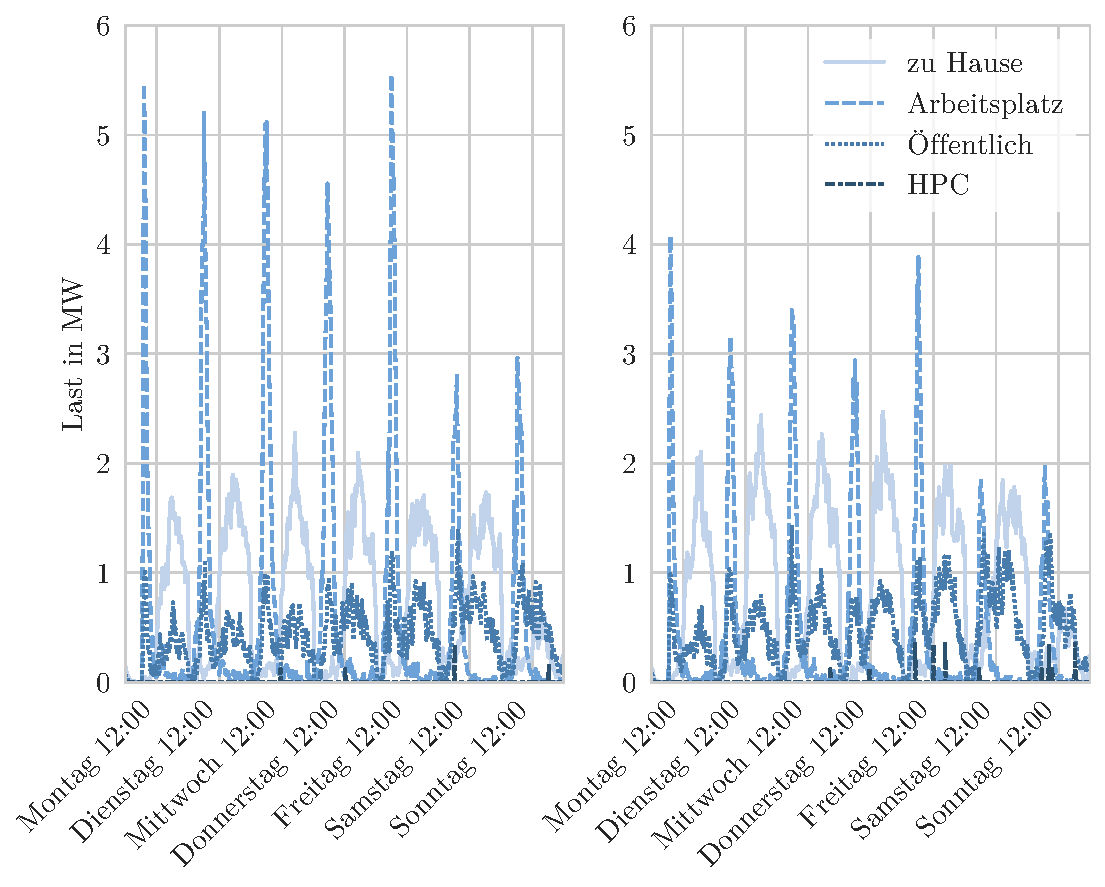
\includegraphics[width=\textwidth]{Bilder/example_load_profile}
    \caption[E-Pkw-Lastprofil für Referenz-Laden im Netz \num{176} über eine Woche im Antriebswende-Szenario und der \SzeFirmenparkplatz]{E-Pkw-Lastprofil (netzseitige Last; inkl. Umwandlungsverluste) für Referenz-Laden im Netz \(176_{\text{PV}}\) über eine Woche im Antriebswende-Szenario (links) und der \SzeFirmenparkplatz (rechts)}\label{fig:example_load_profile}
\end{figure}

Die Lastgänge \zH und \Firmeparkplatz entsprechen den Ladevorgängen im privaten Bereich.
Unter dem Lastgang \oeffen sind hingegen alle öffentlichen Ladevorgänge mit Ausnahme der Schnellladevorgänge (\gls{HPC}) zusammengefasst.
Deutlich zu erkennen ist die hohe Gleichzeitigkeit am Vormittag aufgrund des Wegezwecks \Arbeitdot.
Auch die Rückkehr zum Wohnort ist ab dem frühen Nachmittag in den Lastgängen \zH und im öffentlichen Raum deutlich zu erkennen.
Weiterhin kommt es ab Mittags zu mehr Fahrten der Wegezwecke \Einkaufdot, \Erledigung und \Freizeitdot, welche sich ebenfalls in dem Lastgang \glqq Öffentlich\grqq{} niederschlagen.
Schnellladevorgänge treten unregelmäßig im Verlauf der Woche auf.
Vor allem am Sonntag kommt es zu deutlich geringeren Anteilen von Ladevorgängen \zH und am \Firmeparkplatzdot, wodurch das Flexibilisierungspotential am Wochenende geringer ausfällt.
Gegenüber dem Antriebswende-Szenario sinkt die Höchstlast in der \SzeFirmenparkplatzdot, jedoch sinkt auch das Flexibilisierungspotential bei einem annähernd gleichbleibendem Energiebedarf durch die Verschiebung der Ladevorgänge in den öffentlichen Raum.\medskip

Die entsprechenden Dauerlastkurven für die Gemeinde über eine Woche (s. \autoref{fig:example_load_curve}) zeigen deutlich die dominante Rolle der Hochlastphase, die aufgrund der hohen Gleichzeitigkeit des Wegezwecks \Arbeit vor allem am \Firmeparkplatz aber auch im öffentlichen Raum auftritt.
So wird im Antriebswende-Szenario eine Spitzenlast von \SI{14.8}{\mw} erreicht und in der \SzeFirmenparkplatz von nur \SI{11.3}{\mw}.
Dem Netz \(176_{\text{PV}}\) werden im Antriebswende-Szenario \SI{26359}{\FZ} zugeordnet, welches einem Verhältnis von Spitzenlast zu Fahrzeugen von \SIrange[range-phrase=~bzw.~]{0.56}{0.43}{\kWperFZ} entspricht.
Zum Vergleich wurde in der \textit{Kurzstudie Elektromobilität} für den \gls{NEP} \cite{Ebner2019} für \SI{12}{\MioStk} innerhalb eines Jahres eine Spitzenlast von \SI{12}{\gw} ermittelt, welches einem Verhältnis von \SI{1.00}{\kWperFZ} entspricht.
Für eine mittlere Woche liegt die Spitzenlast in der \textit{Kurzstudie Elektromobilität} bei \SI{9}{\gw} und somit bei \SI{0.75}{\kWperFZ}.
Die Spitzenlast wird nach der \textit{Kurzstudie Elektromobilität} in der Regel am Nachmittag erreicht, da im Vergleich zu dieser Arbeit deutlich mehr Ladevorgänge \zH stattfinden.
Hierdurch ergibt sich innerhalb der Woche am Abend eine besonders hohe Gleichzeitigkeit beim Laden \zHdot, während in der durchgeführten Simulation dieser Arbeit täglich zwei Leistungsspitzen mit einer insgesamt geringeren Gleichzeitigkeit am Morgen und am Nachmittag auftreten.
Das Ergebnis liegt somit in einer ähnlichen Dimension und die Ergebnisse der Simulation können als plausibel angesehen werden.

\begin{figure}[H]
    \centering
    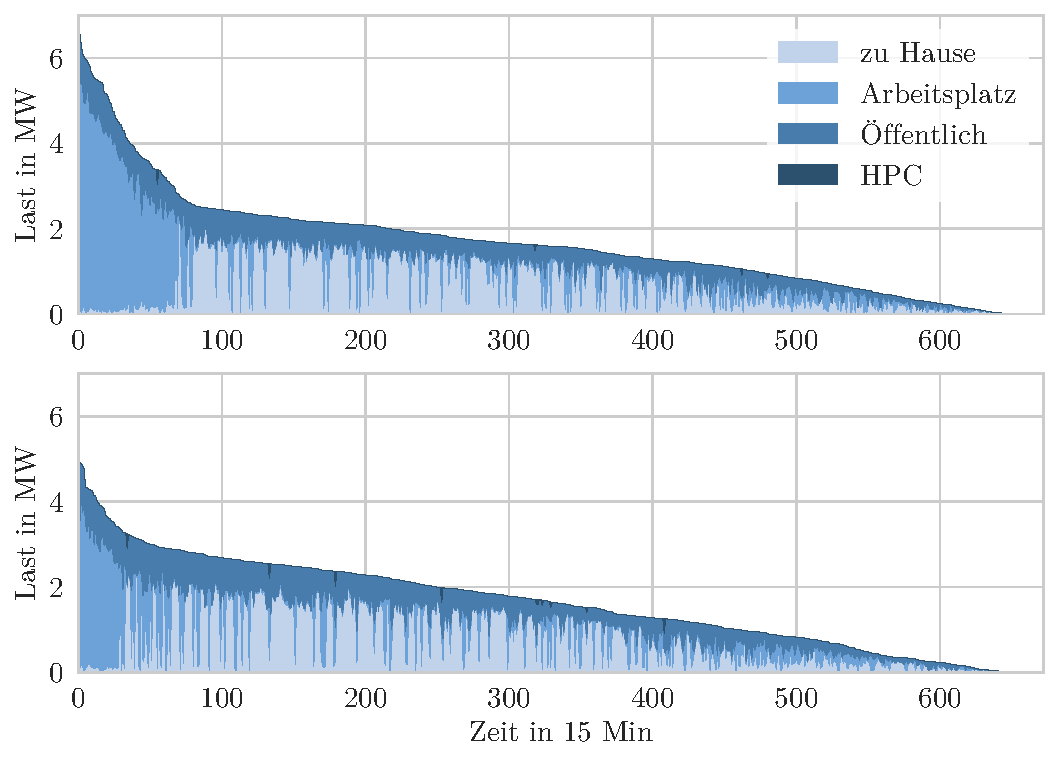
\includegraphics[width=0.9\textwidth]{Bilder/example_load_duration_curve}
    \caption{E-Pkw-Dauerlastkurve für Referenz-Laden im Netz \num{176} über eine Woche im Antriebswende-Szenario (oben) und der \SzeFirmenparkplatz (unten)}\label{fig:example_load_curve}
\end{figure}

Zum Zeitpunkt der Erstellung der Fahrtprofile war es noch nicht möglich, einen längeren Zeitraum als eine Woche am Stück zu simulieren.
Durch die Zuordnung eines zufälligen Eingangs-\gls{SOC} für einige Fahrzeuge (s. \autoref{chap:simbev_theo}) fällt der Ladebedarf am Montag nicht deutlich aus der Reihe.
Jedoch kann hierdurch ein weiterer Effekt nicht verhindert werden.
Bei Fahrzeugen, welche weder einen festen Ladepunkt \zH oder an \Firmeparkplaetzen zugewiesen bekommen haben, fällt der \gls{SOC} im Laufe der Woche langsam ab.
Hierdurch kommt es durch die Abhängigkeit der Ladewahrscheinlichkeit vom \gls{SOC} zu einer Zunahme des Ladebedarfs im öffentlichen Raum im Verlaufe der Woche.
Es ist zu vermuten, dass dies weiterhin dazu führt, dass Ladevorgänge an Schnellladeinfrastruktur un­ter­re­prä­sen­tiert dargestellt werden.


\subsection{Verteilung der Ladevorgänge auf die Ladeinfrastruktur}\label{chap:distribute_demand_ev}

Innerhalb dieses Kapitels werden die Ergebnisse der Verteilung der Ladevorgänge auf konkrete Ladestationen beschrieben.
Hierbei soll vor allem herausgestellt werden, wie sich der Ladebedarf auf die Spannungsebenen verteilt und ob es zu starken lokalen Konzentrationen des Ladebedarfs kommt.\medskip

Die Ermittlung der möglichen Anschlusspunkte nach \autoref{chap:theo_distribution} liefert je \gls{MS}-Netz eine große Anzahl an möglichen Netzanschlusspunkten.
Anschließend werden den Anschlusspunkten Ladepunkte und Ladevorgänge zugeordnet, um die Anschlussleistung zu bestimmen und den Ladebedarf zu regionalisiern.
In \autoref{fig:cps_in_grid} finden sich beispielhaft die ermittelten Netzanschlusspunkte für Ladeinfrastruktur innerhalb des Netzes \(176_{\text{PV}}\) für das Antriebswende-Szenario für Ladeinfrastruktur zu Hause, auf Firmenparkplätzen, Normalladeinfrastruktur im öffentlichen Raum und für Schnellladeinfrastruktur (\gls{HPC}).
Es wird deutlich, dass die Ladeinfrastruktur \zH die meisten Netzanschlusspunkte aufweist, während für die Schnellladeinfrastruktur nur wenige Netzanschlusspunkte benötigt werden.

\begin{figure}[H]
    \centering
    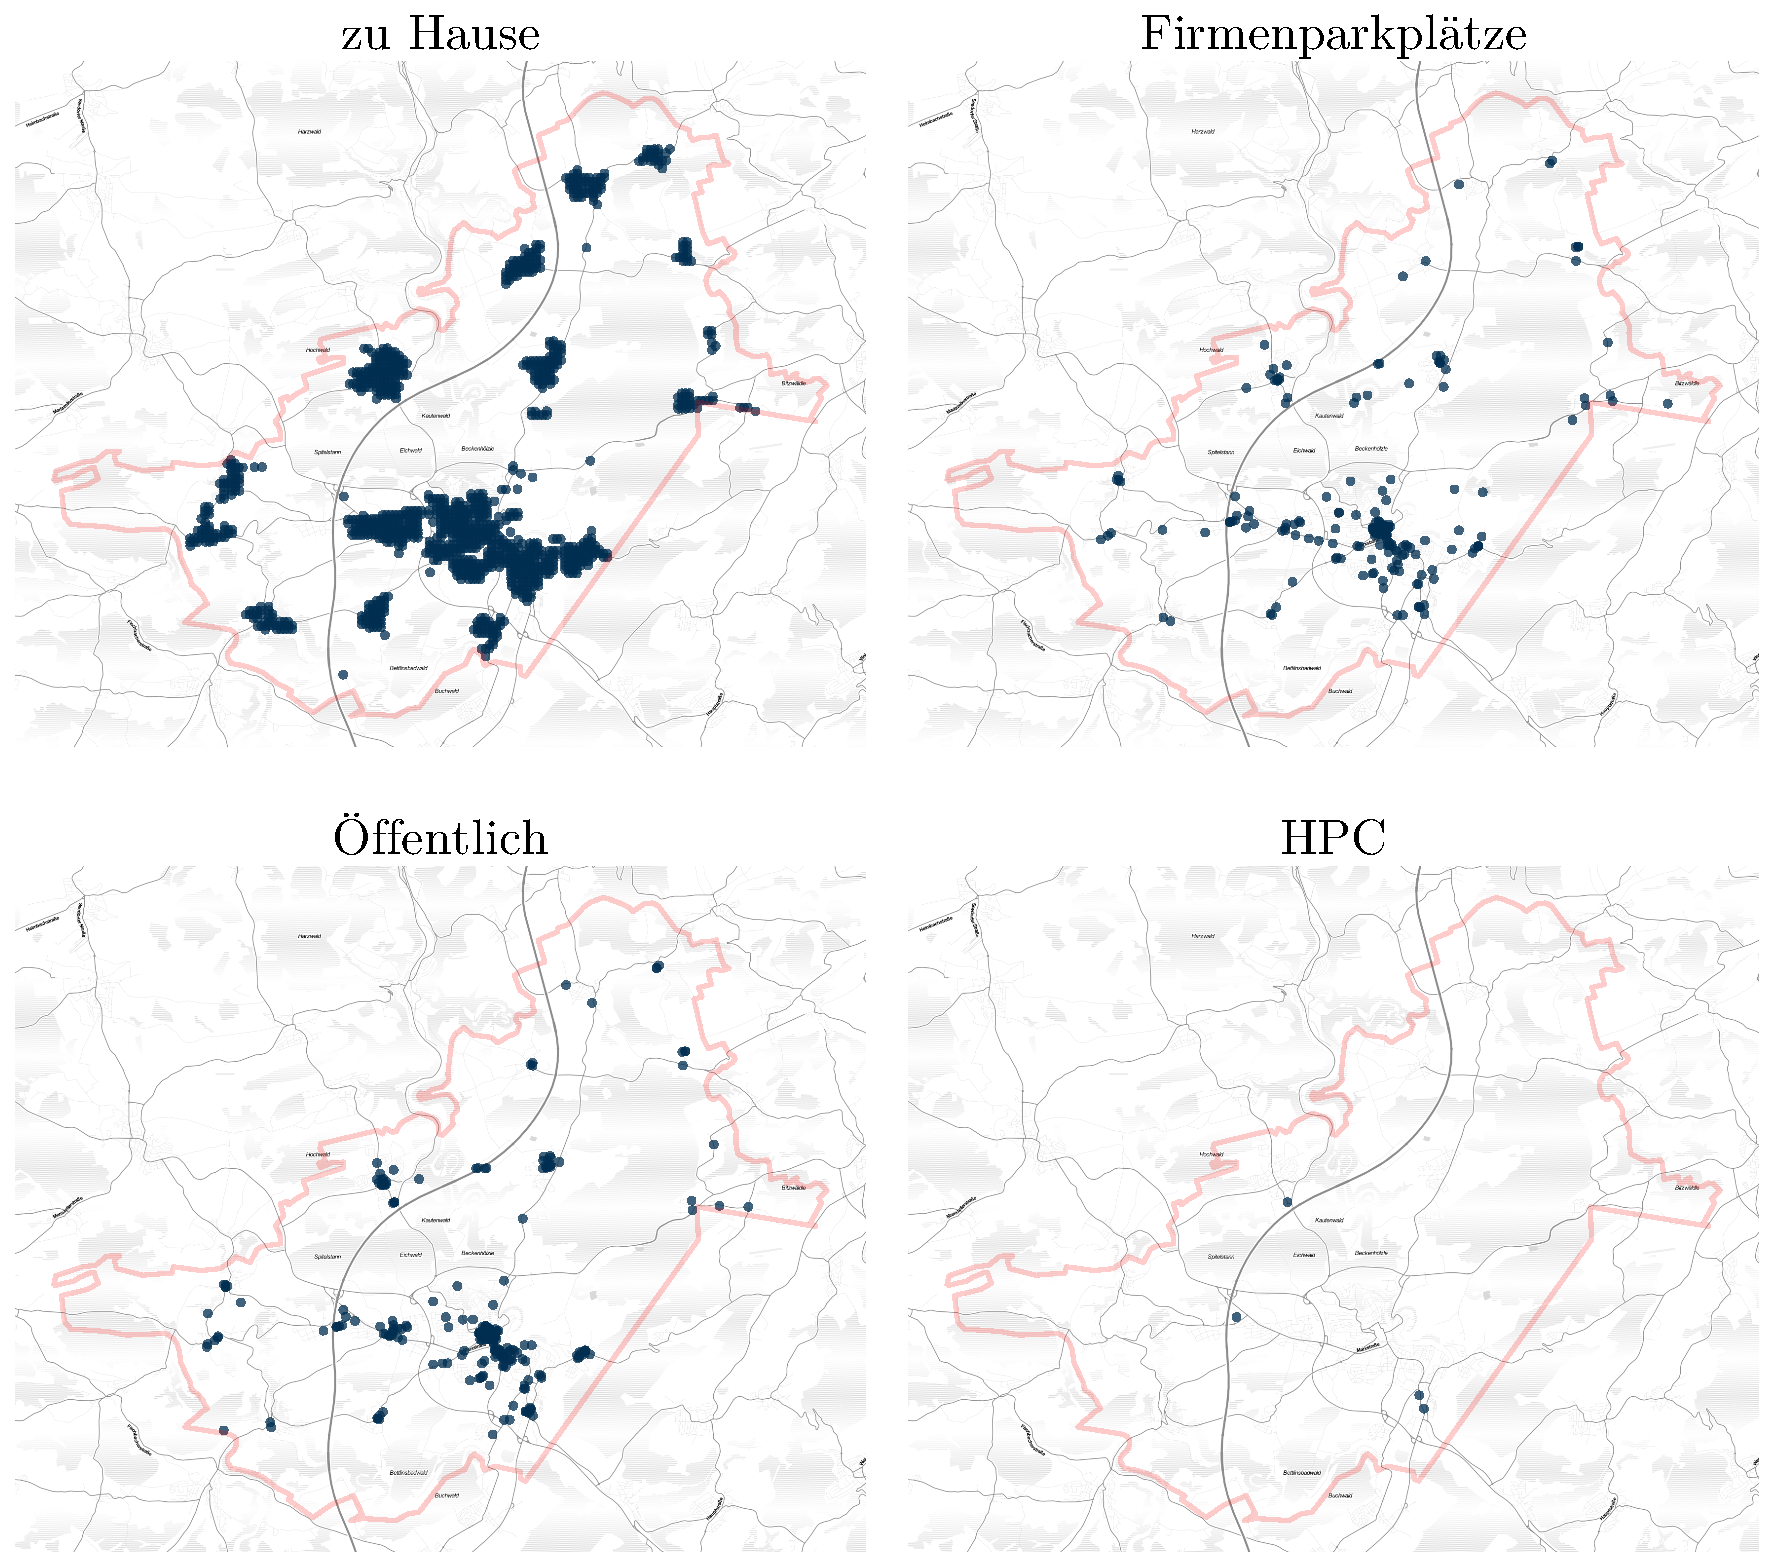
\includegraphics[width=\textwidth]{Bilder/cps_in_grid_176}
    \caption[Geographische Verteilung der ermittelten und zugewiesenen Netzanschlusspunkte für Ladeinfrastruktur im Netz \num{176} für das Antriebswende-Szenario je Lade use case]{Geographische Verteilung der ermittelten und zugewiesenen Netzanschlusspunkte für Ladeinfrastruktur im Netz \(176_{\text{PV}}\) für das Antriebswende-Szenario je Lade use case}\label{fig:cps_in_grid}
\end{figure}

Neben der geographischen Lokalisation der Ladeinfrastruktur ist es für die Netzuntersuchungen entscheidend, ob die Ladeinfrastruktur in der \gls{NS}- oder \gls{MS}-Ebene angeschlossen wird.
Erfolgt der Anschluss in der \gls{NS}-Ebene, dann werden sowohl die Betriebsmittel der \gls{NS}- und \gls{MS}-Ebene belastet, während bei einem Anschluss in der \gls{MS}-Ebene auch nur diese betroffen ist.
Außerdem findet bei einem Anschluss von privater Ladeinfrastruktur in der \gls{MS}-Ebene auch bei der Referenz-Ladestrategie reduziertes Laden statt (s. \autoref{chap:theo_strategies}).
In \autoref{tab:lvConnectionShare} findet sich der Anteil des in der \gls{NS}-Ebene anfallenden Energiebedarfs vom Gesamtenergiebedarf der Ladeinfrastruktur im \gls{MS}-Netz.
Es wird deutlich, dass der Anteil von Ladeinfrastruktur in der \gls{MS}-Ebene mit einer steigenden Zahl von Fahrzeugen zunimmt, da eine steigende Anzahl von Ladepunkten auf eine gleichbleibende Anzahl von möglichen Anschlusspunkten verteilt werden muss und somit die kumulierte Leistung der Ladestationen ansteigt.
Gleichzeitig zeigt sich, dass in der \SzeFirmenparkplatz der Anteil von Ladeinfrastruktur in der \gls{MS}-Ebene deutlich geringer ausfällt als im Antriebswende-Szenario, trotz einer gleichen Anzahl an \gls{EPKW}.
Dies lässt sich damit erklären, dass neben der öffentlichen Ladeinfrastruktur vor allem Ladeinfrastruktur des \UC \Firmeparkplatz einen Anschluss in der \gls{MS}-Ebene benötigt.
Da im Antriebswende-Szenario mehr Ladevorgänge des Wegezwecks \Arbeit auf eine gleichbleibende Anzahl von möglichen Anschlusspunkten für Ladeinfrastruktur des \UC \Firmeparkplatz verteilt werden müssen, fällt die Anschlussleistung dieser Ladeinfrastruktur deutlich höher aus und macht somit einen Anschluss in der \gls{MS}-Ebene nötig.

{
\renewcommand{\arraystretch}{1.2}% grßerer Zeilenabstand
\sisetup{range-phrase=~{--}~}% Gedankenstrich statt "bis" bei SIrange
\begin{table}[H]
	\begin{center}
		\caption{Anteil des in der NS-Ebene anfallenden Energiebedarfs vom Gesamtenergiebedarf der Ladeinfrastruktur je Szenario}
		\begin{tabu} to \textwidth {X[0.5] X[1, r] X[1, r] X[1.2, r] X[1.2, r]}
			\hline
			Netz ID    & NEP C \num{2035}    & Referenz            & Antriebswende       & \glqq Firmenparkplatz\grqq \\ \hline
			\num{176}  & \SI{98.0}{\percent} & \SI{92.9}{\percent} & \SI{82.0}{\percent} & \SI{91.3}{\percent}        \\
			\num{1056} & \SI{99.8}{\percent} & \SI{99.5}{\percent} & \SI{94.0}{\percent} & \SI{97.9}{\percent}        \\
			\num{1690} & \SI{99.8}{\percent} & \SI{97.0}{\percent} & \SI{86.5}{\percent} & \SI{92.9}{\percent}        \\
			\num{1811} & \SI{99.9}{\percent} & \SI{98.7}{\percent} & \SI{90.0}{\percent} & \SI{95.2}{\percent}        \\
			\num{177}  & \SI{96.6}{\percent} & \SI{86.8}{\percent} & \SI{77.8}{\percent} & \SI{86.7}{\percent}        \\
			\num{2534} & \SI{99.7}{\percent} & \SI{97.4}{\percent} & \SI{80.8}{\percent} & \SI{91.4}{\percent}        \\ \hline
		\end{tabu}
		\label{tab:lvConnectionShare}
	\end{center}
	\vspace{-3mm}%Put here to reduce too much white space after your table
\end{table}
}

In \autoref{tab:largestLVGridShare} ist die Anzahl an \gls{NS}-Netzen je \gls{MS}-Netz und der maximale Anteil eines \gls{NS}-Netzes am Gesamtenergiebedarf der Ladeinfrastruktur in der \gls{NS}-Ebene in allen betrachteten Szenarien dargestellt.
Hierbei wird deutlich, dass es in einigen \gls{MS}-Netzen zu einer starken lokalen Konzentration an Ladeinfrastruktur kommt.
So fallen beispielsweise im Netz \(176_{\text{PV}}\) im NEP C~\num{2035} Szenario \SI{36.3}{\percent} des Energiebedarfs der Ladeinfrastruktur in der \gls{NS}-Ebene innerhalb eines einzigen \gls{NS}-Netzes an.
Diese starke Konzentration spiegelt sich in \autoref{fig:cps_in_grid} durch eine starke Konzentration der Ladeinfrastruktur in den bewohnten Regionen wider.
In der Realität würde es bei solch starken lokalen Konzentrationen vermutlich zu einem Netzneubau kommen, welcher innerhalb dieser Arbeit nicht abgebildet werden kann.

{
\renewcommand{\arraystretch}{1.2}% grßerer Zeilenabstand
\sisetup{range-phrase=~{--}~}% Gedankenstrich statt "bis" bei SIrange
\begin{table}[H]
	\begin{center}
		\caption{Anzahl der NS-Netze je MS-Netzgebiet und maximal anfallender Energieanteil eines NS-Netzes am Gesamtenergiebedarf der Ladeinfrastruktur in den NS-Netzen in allen betrachteten Szenarien}
		\begin{tabu} to 0.7\textwidth {X[0.75] X[1, r] X[1.5, r]}
			\hline
			Netz ID    & Anzahl NS-Netze & Maximaler Energieanteil 			\\ \hline
			\num{176}  & \num{105}       & \SI{36.3}{\percent}              \\
			\num{1056} & \num{130}       & \SI{12.9}{\percent}              \\
			\num{1690} & \num{179}       & \SI{11.4}{\percent}              \\
			\num{1811} & \num{381}       & \SI{7.9}{\percent}               \\
			\num{177}  & \num{56}        & \SI{26.5}{\percent}              \\
			\num{2534} & \num{9}         & \SI{62.3}{\percent}              \\ \hline
		\end{tabu}
		\label{tab:largestLVGridShare}
	\end{center}
	\vspace{-3mm}%Put here to reduce too much white space after your table
\end{table}
}


\subsection{Auswirkungen der Ladestrategien}\label{chap:results_charging_strategies}

Innerhalb dieses Kapitels soll der Einfluss der Ladestrategien auf die Spitzenlast im Last- und Rückspeisefall aufgezeigt werden, sowie die Veränderung des Lastprofils des Ladebedarfs der \gls{EPKW} aufgrund der Ladestrategien dargestellt werden.
Im Rahmen der Netzuntersuchungen kommt den Zeitreihen der Last der \glspl{EPKW} die größte Bedeutung zu, da die Last und Erzeugung aller anderen Verbraucher und Erzeuger nicht variiert wird.
Das Ziel der Ladestrategien (s. \autoref{chap:theo_strategies}) ist es, die Netzbelastung möglichst gering zu halten.
Bei den Ladegruppen und dem reduzierten Laden soll dies durch ein präventives Lademanagement und bei dem Residuallast-Laden durch ein aktives Lademanagement erreicht werden.

\begin{figure}[H]
    \centering
    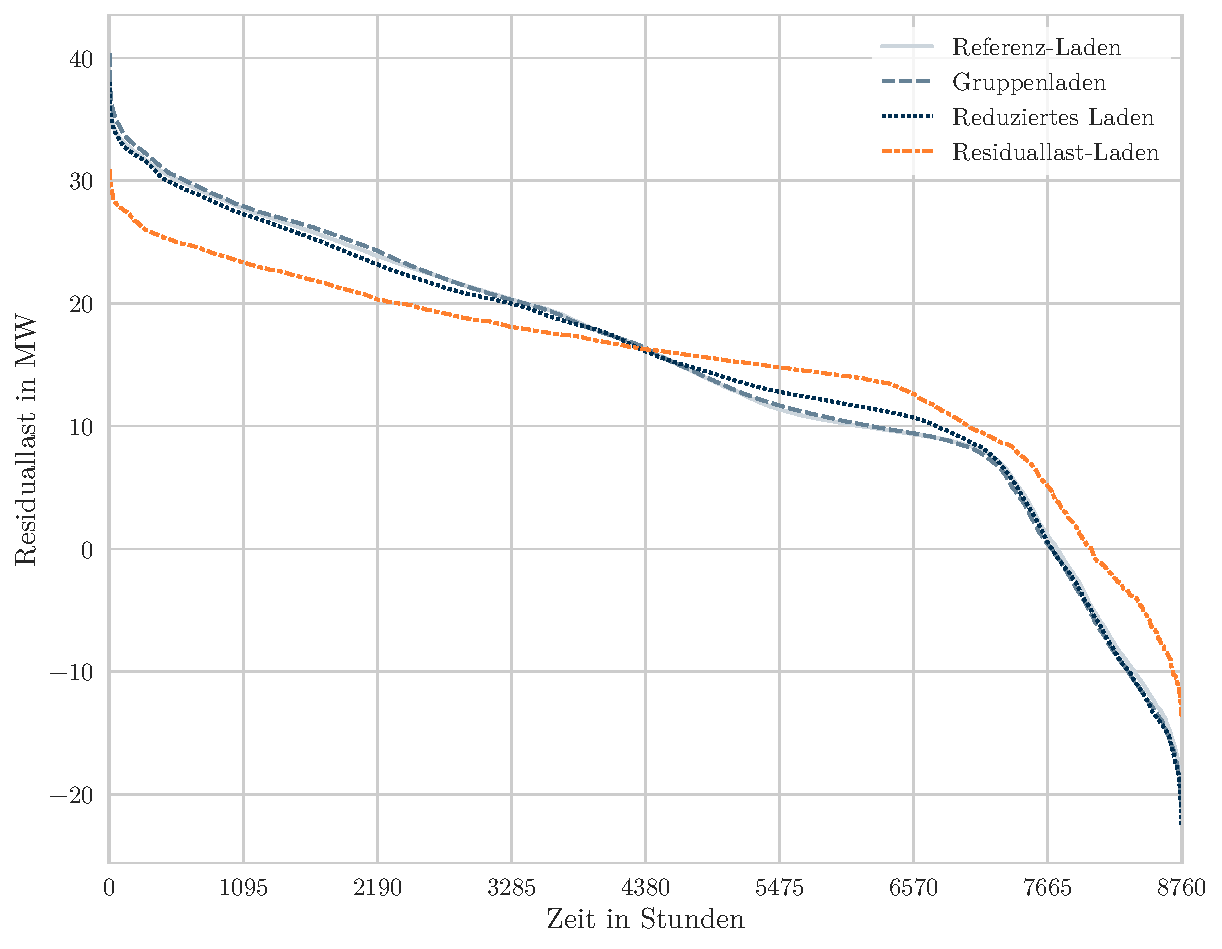
\includegraphics[width=1\textwidth]{Bilder/example_resiual_load}
    \caption{Residuallast im Netzgebiet \num{176} für das Antriebswende-Szenario}\label{fig:residual_load}
\end{figure}

\autoref{fig:residual_load} zeigt beispielhaft die Residuallast im Netz \(176_{\text{PV}}\) in Abhängigkeit von der Ladestrategie im Antriebswende-Szenario.
Dabei zeigt sich deutlich, dass nur die Residuallast-Ladestrategie zu einer deutlichen Glättung der Residuallastkurve führt.
Dies bestätigt sich in einer Betrachtung der Veränderung der Spreizung zwischen dem maximalen Last- und Rückspeisefall in den Referenznetzgebieten aufgrund der Ladestrategien in \autoref{tab:ResidualLoadSpread}.
Demnach kann durch die Residuallast-Ladestrategie die Spreizung vor allem in den \gls{PV}- und Last-domninierten Netzen stark reduziert werden.
In den Wind-dominierten Netzen fällt die Reduktion geringer aus, da das Verhältnis zwischen Einspeisung und Ladebedarf deutlich größer ausfällt und damit der Einfluss des Ladebedarfs auf die Residuallast abnimmt.
Die präventiven Ladestrategien zeigen hingegen keinen deutlichen Einfluss auf die Residuallast in den Referenznetzgebieten.
Insgesamt führen die präventiven Ladestrategien gegenüber dem Referenz-Laden sogar zu einer leichten Erhöhung der Spreizung.
Hierbei kommt es bei den Ladegruppen eher zu einer Erhöhung der Last im Lastfall, während es durch das reduzierte Laden zu einer Erhöhung im Rückspeisefall kommt, wobei auf diesen Effekt detailliert in \autoref{chap:cur_results} eingegangen wird .

{
\renewcommand{\arraystretch}{1.2}% grßerer Zeilenabstand
\sisetup{range-phrase=~{--}~}% Gedankenstrich statt "bis" bei SIrange
\begin{table}[H]
	\begin{center}
		\caption{Spreizung der Residuallast zwischen dem maximalen Last- und Rückspeisefall in den Referenznetzgebieten und die prozentuale Veränderung der Spreizung aufgrund der Ladestrategien im Antriebswende-Szenario}
		\begin{tabu} to \textwidth {X[0.5] X[1, r] X[1, r] X[1.2, r] X[1.2, r]}
			\toprule
			Netz ID    & Referenz-Laden  & Ladegruppen                               & Reduziertes Laden                          & Residuallast-Laden                         \\ \midrule
			\(176_{\text{PV}}\)  & \SI{58.4}{\mw}  & \SI[retain-explicit-plus]{+5.3}{\percent} & \SI[retain-explicit-plus]{+3.6}{\percent}  & \SI[retain-explicit-plus]{-24.0}{\percent} \\
			\(1056_{\text{PV}}\) & \SI{84.5}{\mw}  & \SI[retain-explicit-plus]{+0.0}{\percent} & \SI[retain-explicit-plus]{+0.6}{\percent}  & \SI[retain-explicit-plus]{-10.2}{\percent} \\
			\(1690_{\text{W}}\) & \SI{113.5}{\mw} & \SI[retain-explicit-plus]{+0.1}{\percent} & \SI[retain-explicit-plus]{+0.8}{\percent}  & \SI[retain-explicit-plus]{-5.7}{\percent}  \\
			\(1811_{\text{W}}\) & \SI{98.4}{\mw}  & \SI[retain-explicit-plus]{+0.3}{\percent} & \SI[retain-explicit-plus]{+0.4}{\percent}  & \SI[retain-explicit-plus]{-7.0}{\percent}  \\
			\(177_{\text{L}}\)  & \SI{36.6}{\mw}  & \SI[retain-explicit-plus]{+4.5}{\percent} & \SI[retain-explicit-plus]{-0.2}{\percent}  & \SI[retain-explicit-plus]{-25.5}{\percent} \\ \bottomrule
		\end{tabu}
		\label{tab:ResidualLoadSpread}
	\end{center}
	\vspace{-3mm}%Put here to reduce too much white space after your table
\end{table}
}

In \autoref{fig:residual_load_diff} ist die Veränderung der Last der \glspl{EPKW} im Netz \(176_{\text{PV}}\) über ein Jahr in Abhängigkeit von den verschiedenen Ladestrategien dargestellt.
Dabei zeigt die Darstellung der Referenz-Ladestrategie (oben links) die Last der \glspl{EPKW} über ein Jahr, während in den anderen drei Darstellungen die Differenz der jeweiligen Ladestrategie zum Referenz-Laden abgebildet wird.
Da im Antriebswende-Szenario im Netz \(176_{\text{PV}}\) \SI{18}{\percent} des Ladebedarfs in der \gls{MS}-Ebene anfallen (vgl. \autoref{tab:lvConnectionShare}), kommt es beim Referenz-Laden bereits zu einem erhöhten Anteil an reduzierten Ladevorgängen vor allem bei dem \UC \Firmeparkplatz und nur selten im \UC \zH (s. \autoref{chap:theo_strategies}).
Bei den Ladegruppen werden die Ladevorgänge zeitlich weniger gestreckt als bei reduzierten Ladevorgängen, weshalb gegenüber dem Referenz-Laden eine Zunahme der Last am Morgen festzustellen ist.
Bei dem \UC \zH kommt es hingegen beim Referenz-Laden nur zu wenigen reduzierten Ladevorgängen.
Gegenüber ungesteuerten Ladevorgängen werden die Ladevorgänge bei den Ladegruppen stärker zeitlich gestreckt, weshalb es vorerst am frühen Nachmittag zu einem reduzierten Ladebedarf kommt, welcher anschließend bis in die Nacht hinein nachgeholt wird.
Bei dem reduzierten Laden finden gegenüber dem Referenz-Laden die Ladevorgänge der \UCs \zH und \Firmeparkplatzdot, welche innerhalb der \gls{NS}-Ebene anfallen, bei reduzierten Ladeleistungen statt.
Hierdurch kommt es vor allem am Morgen zu einer deutlichen Senkung des Ladebedarfs des \UCs \Firmeparkplatzdot, welches im Gegenzug den Ladebedarf im Verlaufe des Vormittags erhöht.
Ab der Mittagszeit kommt es vermehrt zu Ladevorgängen des \UCs \zHdot, weshalb der Ladebedarf in dieser Zeit reduziert wird.
Anschließend kommt es zu einer stärkeren Zunahme des Ladebedarfs in der Nacht, da viele Ladevorgänge zeitlich bis in die Nacht gestreckt werden.

\begin{figure}[H]
    \centering
    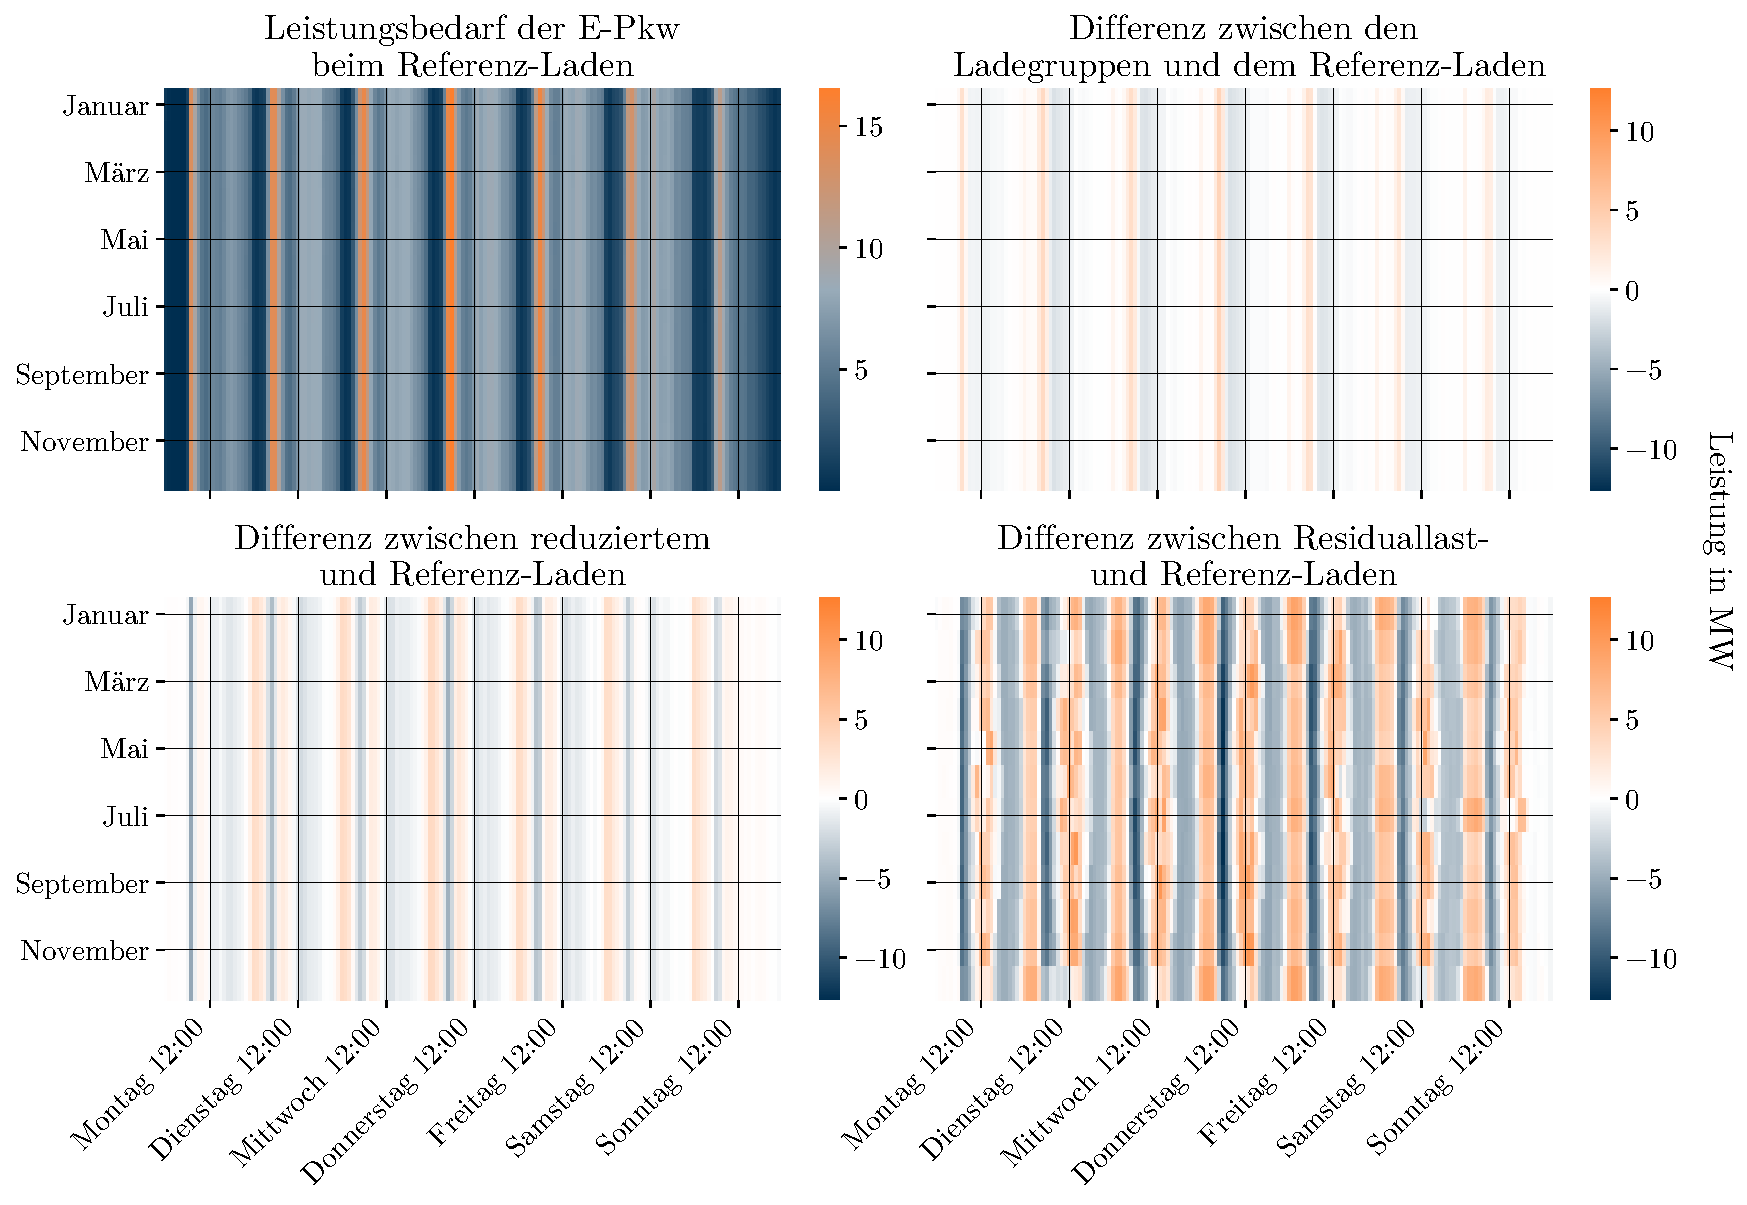
\includegraphics[width=\textwidth]{Bilder/residual_load_diff}
    \caption[Veränderung des durchschnittlichen stündlichen Leistungsbedarfs von E-Pkw je Wochentag im Netz \num{176} für das Antriebswende-Szenario über ein Jahr in Abhängigkeit von der Ladestrategie]{Veränderung des durchschnittlichen stündlichen Leistungsbedarfs von E-Pkw je Wochentag im Netz \(176_{\text{PV}}\) für das Antriebswende-Szenario über ein Jahr in Abhängigkeit von der Ladestrategie}\label{fig:residual_load_diff}
\end{figure}

Die stärksten Veränderungen werden bei der Residuallast-Ladestrategie festgestellt.
Da es sich bei dem Netz \(176_{\text{PV}}\) um ein \gls{PV}-dominiertes Netz handelt, kommt es zu einer starken Verschiebung der Ladevorgänge in die Mittagszeit.
Auch kommt es zu einer deutlichen Verschiebung der Last in die Schwachlastzeit nach Mitternacht, während die Last am Vor- und Nachmittag abnimmt.
Bei den anderen \gls{MS}-Netzen lässt sich für die Ladegruppen und das reduzierte Laden das gleiche Verhalten feststellen.
Aufgrund des \gls{PV}-Anteils in den Wind- und Last-dominierten Netzen kommt es auch bei diesen Netzklassen bei dem Residuallast-Laden zu einer Verschiebung der Last in die Mittagszeit.
Ebenfalls lässt sich eine Verschiebung in die nächtliche Schwachlastzeit feststellen.
Insgesamt zeigt sich bei den Wind-dominierten jedoch aufgrund der Fluktuation in der Erzeugung der Wind-Kapazitäten ein unregelmäßigeres Bild als in den \gls{PV}- und Last-dominierten Netzen.


\subsection{Abregelungsbedarf innerhalb der untersuchten Netze}\label{chap:cur_results}

In diesem Abschnitt werden die Ergebnisse der Ermittlung des Abregelungsbedarfs innerhalb der fünf untersuchten \gls{MS}-Netze dargestellt.
Dabei wird getrennt auf die drei Netz-Kategorien \gls{PV}-, Wind- und Last-dominiert eingegangen, um eine Aussage über die Wirksamkeit der Ladestrategien innerhalb der verschiedenen Netz-Kategorien treffen zu können.
Hierzu werden die zwei Wochen mit der minimalen (kurz: Woche~MIN) bzw. maximalen (kurz: Woche~MAX) durchschnittlichen Residuallast je \gls{MS}-Netz untersucht, um eine möglichst hohe Bandbreite an Einspeise- und Lastfällen abzudecken.
Die entsprechenden Zeiträume finden sich in \autoref{tab:extreme_weeks}, wobei die untersuchten Wochen und das fiktive betrachtete Jahr mit einem Montag beginnen.

{
\renewcommand{\arraystretch}{1.2}% grßerer Zeilenabstand
\sisetup{range-phrase=~{--}~}% Gedankenstrich statt "bis" bei SIrange
\begin{table}[H]
	\begin{center}
		\caption{Untersuchte Wochen je Netzgebiet}
		\begin{tabu} to 0.6\textwidth {X[0.5] X[1, r] X[1, r]}
			\toprule
			Netz ID	   & Woche A                         & Woche B                         \\ \midrule
			\num{176}  & \(16.04. \text{ {--} } 22.04.\) & \(08.01. \text{ {--} } 14.01.\) \\
			\num{1056} & \(30.04. \text{ {--} } 06.05.\) & \(08.01. \text{ {--} } 14.01.\) \\
			\num{1690} & \(03.12. \text{ {--} } 09.12.\) & \(29.10. \text{ {--} } 04.11.\) \\
			\num{1811} & \(10.12. \text{ {--} } 16.12.\) & \(24.09. \text{ {--} } 30.09.\) \\
			\num{177}  & \(16.04. \text{ {--} } 22.04.\) & \(10.12. \text{ {--} } 16.12.\) \\
			\num{2534} & \(16.04. \text{ {--} } 22.04.\) & \(03.12. \text{ {--} } 09.12.\) \\ \bottomrule
		\end{tabu}
		\label{tab:extreme_weeks}
	\end{center}
	\vspace{-3mm}%Put here to reduce too much white space after your table
\end{table}
}

Innerhalb der betrachteten Szenarien, Ladestrategien und Wochen schwankt der Abregelungsbedarf von nicht-\glspl{FEE} Anlagen nur in einem sehr geringen Maße, weshalb der Fokus der Betrachtung der erzeugungsseitigen Abregelungsergebnisse auf den \gls{FEE} Anlagen liegt.
Dies lässt sich dadurch begründen, dass die Abregelung der nicht-\gls{FEE} Anlagen in den betrachteten Netzen in der Regel aufgrund von Restriktionen in der \gls{NS}-Ebene erfolgt.
Da es sich bei den nicht-\gls{FEE} Anlagen ausschließlich um Biomasse- und Wasserkraftwerke handelt, findet sich innerhalb der betroffenen \gls{NS}-Netze in der Regel keine oder nur wenig Ladeinfrastruktur für \gls{EPKW}.
Hierdurch kommt es nur sehr selten zu einem Einfluss auf den Abregelungsbedarf von nicht-\gls{FEE} Anlagen.
Die vollständigen Ergebnisse für die Ermittlung des Abregelungsbedarfs finden sich im Anhang in den Netz-Steckbriefen ab \autoref{tab:steckbrief_176_A}.


\subsubsection{PV-dominierte Netze}

Die \gls{PV}-dominierten Netze \(176_{\text{PV}}\) und \(1056_{\text{PV}}\) besitzen stark unterschiedliche Charakteristika.
So weist das Netz \(176_{\text{PV}}\) im Antriebswende-Szenario in der Woche~MIN ein Verhältnis zwischen der Einspeisung von \glspl{FEE} und dem Ladebedarf der \glspl{EPKW} von etwa \(2:1\) auf, während dieses Verhältnis im Netz \(1056_{\text{PV}}\) bei etwa \(11:1\) liegt.
Auch weist das Netz \(176_{\text{PV}}\) eine deutlich größere Einspeisung von nicht-\gls{FEE} Anlagen auf und der Verbrauch der sonstigen Lasten ist mehr als dreimal so hoch wie im Netz \(1056_{\text{PV}}\).
Eine Auflistung der wichtigsten Eckdaten für die Woche~MIN beider Netze findet sich in \autoref{tab:pv_dominated_week_a_char} und der Ladebedarf je \gls{MS}-Netz und Szenario findet sich in \autoref{tab:pv_dominated_epkw_demand}.

{
\renewcommand{\arraystretch}{1.2}% grßerer Zeilenabstand
\sisetup{range-phrase=~{--}~}% Gedankenstrich statt "bis" bei SIrange
\begin{table}[H]
	\begin{center}
		\caption{Einspeisung von fEE und nicht-fEE sowie der Bedarf von sonstigen Lasten in den PV-dominierten Netzen in Woche~MIN}
		\begin{tabu} to 0.7\textwidth {X[2] X[1, r] X[1, r]}
			\toprule
											  & Netz \(176_{\text{PV}}\) & Netz \(1056_{\text{PV}}\) \\ \midrule
			Einspeisung fEE in \si{\mwh}      & \num{2262.2}   & \num{4054.8}    \\
			Einspeisung Sonstige in \si{\mwh} & \num{1459.8}   & \num{254.5}     \\
			Bedarf Sonstige  in \si{\mwh}     & \num{4196.8}   & \num{1318.0}    \\ \bottomrule
		\end{tabu}
		\label{tab:pv_dominated_week_a_char}
	\end{center}
	\vspace{-3mm}%Put here to reduce too much white space after your table
\end{table}
}

{
\renewcommand{\arraystretch}{1.2}% grßerer Zeilenabstand
\sisetup{range-phrase=~{--}~}% Gedankenstrich statt "bis" bei SIrange
\begin{table}[H]
	\begin{center}
		\caption{Ladebedarf der E-Pkw in den PV-dominierten Netzen je Szenario in Woche~MIN}
		\begin{tabu} to 0.6\textwidth {X[1.5] X[1, r] X[1, r]}
			\toprule
			Ladebedarf in   \si{\mwh} 		& Netz \(176_{\text{PV}}\) & Netz \(1056_{\text{PV}}\) \\ \midrule
			NEP C~\num{2035}                & \num{290.0}    & \num{109.3}     \\
			Referenz                        & \num{519.6}    & \num{193.7}     \\
			Antriebswende                   & \num{987.7}    & \num{368.5}     \\
			\glqq Firmenparkplatz\grqq{}    & \num{974.3}    & \num{363.1}     \\ \bottomrule
		\end{tabu}
		\label{tab:pv_dominated_epkw_demand}
	\end{center}
	\vspace{-3mm}%Put here to reduce too much white space after your table
\end{table}
}

In \autoref{tab:pv_dominated_week_a_epkw_cur} findet sich der ermittelte Abregelungsbedarf des Ladebedarfs und in \autoref{tab:pv_dominated_week_a_load_cur} der sonstigen Lasten für die Netze \(176_{\text{PV}}\) und \(1056_{\text{PV}}\) für die Referenz-Ladestrategie.
Der Abregelungsbedarf von Lasten nimmt erwartungsgemäß mit dem Hochlauf an \gls{EPKW} zu.
Im Netz \(176_{\text{PV}}\) kommt es zu einer extrem hohen Abregelung von bis zu knapp \SI{50}{\percent} des gesamten Ladebedarfs der \gls{EPKW}.
Beispielsweise entfällt in der \SzeFirmenparkplatz der Abregelungsbedarf zu etwa \SI{82}{\percent} auf nur drei \gls{NS}-Netze.
Dieses Ergebnis spiegelt die extreme Konzentration des Ladebedarfs in einigen wenigen \gls{NS}-Netzen innerhalb des Netzes \(176_{\text{PV}}\) nach \autoref{tab:largestLVGridShare} wider und lässt sich auch in den anderen Szenarien beobachten.

Demgegenüber erweist sich das Netz \(1056_{\text{PV}}\) als deutlich stabiler und weist nur einen geringen Abregelungsbedarf des Ladebedarfs von \gls{EPKW} auf.
Aufgrund der geringeren Anzahl an Lademöglichkeiten des \UC \Firmeparkplatz in der \SzeFirmenparkplatzdot, werden die Ladevorgänge gleichmäßiger über den Tag verteilt (vgl. \autoref{fig:example_load_profile} und \autoref{fig:example_load_curve}).
Zusätzlich fällt der Ladebedarf aufgrund der probabilistischen Natur der Simulation und der veränderten Eingangsparameter in der \SzeFirmenparkplatz geringer aus als im Antriebswende-Szenario.
Aus diesen Gründen fällt der Abregelungsbedarf in der \SzeFirmenparkplatz geringer aus als im Antriebswende-Szenario.
Da im Netz \(176_{\text{PV}}\) vor allem \gls{NS}-Netze mit einem hohen Anteil an Ladevorgängen des \UCs \zH von den starken Abregelungen betroffen sind, tritt hierbei ein gegenteiliger Effekt auf und der Abregelungsbedarf erhöht sich in der \SzeFirmenparkplatzdot.

{
\renewcommand{\arraystretch}{1.2}% grßerer Zeilenabstand
\sisetup{range-phrase=~{--}~}% Gedankenstrich statt "bis" bei SIrange
\begin{table}[H]
	\begin{center}
		\caption{Abregelungsbedarf des Ladebedarfs von E-Pkw in den PV-dominierten Netzen je Szenario für die Referenz-Ladestrategie in Woche~MIN}
		\begin{tabu} to 0.6\textwidth {X[1.5] X[1, r] X[1, r]}
			\toprule
			Abregelung in   \si{\mwh}    & Netz \num{176} & Netz \num{1056} \\ \midrule
			NEP C~\num{2035}             & \num{91.2}     & \num{3.3}       \\
			Referenz                     & \num{212.7}    & \num{12.0}      \\
			Antriebswende                & \num{418.1}    & \num{31.9}      \\
			\glqq Firmenparkplatz\grqq{} & \num{470.8}    & \num{24.5}      \\ \bottomrule
		\end{tabu}
		\label{tab:pv_dominated_week_a_epkw_cur}
	\end{center}
	\vspace{-3mm}%Put here to reduce too much white space after your table
\end{table}
}

{
\renewcommand{\arraystretch}{1.2}% grßerer Zeilenabstand
\sisetup{range-phrase=~{--}~}% Gedankenstrich statt "bis" bei SIrange
\begin{table}[H]
	\begin{center}
		\caption{Abregelungsbedarf der sonstigen Lasten in den PV-dominierten Netzen je Szenario für die Referenz-Ladestrategie in Woche~MIN}
		\begin{tabu} to 0.6\textwidth {X[1.5] X[1, r] X[1, r]}
			\toprule
			Abregelung in   \si{\mwh}    & Netz \num{176} & Netz \num{1056} \\ \midrule
			NEP C~\num{2035}             & \num{9.5}      & \num{16.2}      \\
			Referenz                     & \num{10.8}     & \num{19.6}      \\
			Antriebswende                & \num{12.0}     & \num{29.0}      \\
			\glqq Firmenparkplatz\grqq{} & \num{11.8}     & \num{22.9}      \\ \bottomrule
		\end{tabu}
		\label{tab:pv_dominated_week_a_load_cur}
	\end{center}
	\vspace{-3mm}%Put here to reduce too much white space after your table
\end{table}
}

In \autoref{fig:176_1056_cur_load_grid_week_A} findet sich der Einfluss der Ladestrategien auf den Abregelungsbedarf der Lasten (inkl. E-Pkw) für die Netze \(176_{\text{PV}}\) und \(1056_{\text{PV}}\).
Hierbei zeigt sich, dass die Ladegruppen gegenüber dem Referenz-Laden in beiden Netzen keine nennenswerten Vorteile aufweist, während durch das reduzierte Laden der Abregelunsgebdarf deutlich gesenkt werden kann.

\begin{figure}[H]
    \centering
    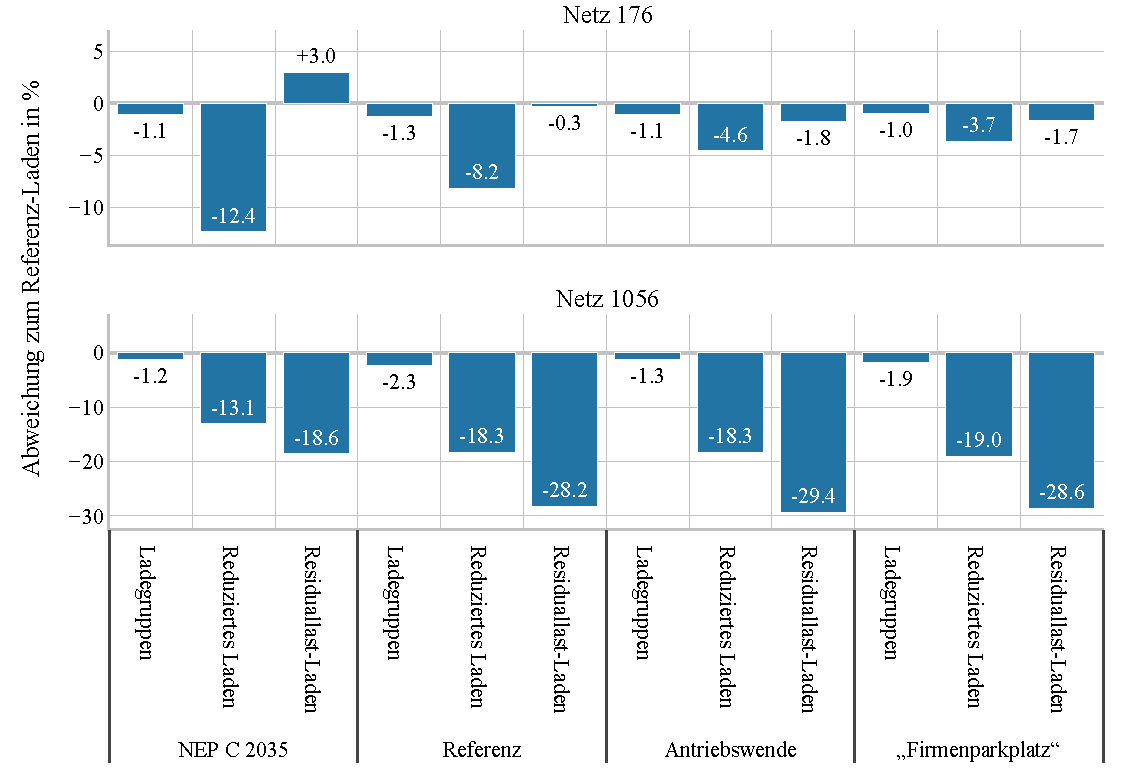
\includegraphics[width=\textwidth]{Bilder/176_1056_cur_load_grid_week_A}
    \caption[Prozentuale Veränderung des Abregelungsbedarfs von allen Lasten in Abhängigkeit von der Ladestrategie in Woche~MIN gegenüber dem Abregelungsbedarf für die Referenz-Ladestrategie je Szenario für die Netze \num{176} und \num{1056}]{Prozentuale Veränderung des Abregelungsbedarfs von allen Lasten in Abhängigkeit von der Ladestrategie in Woche~MIN gegenüber dem Abregelungsbedarf für die Referenz-Ladestrategie je Szenario für die Netze \(176_{\text{PV}}\) (oben) und \(1056_{\text{PV}}\) (unten)}\label{fig:176_1056_cur_load_grid_week_A}
\end{figure}

Im Netz \(176_{\text{PV}}\) nimmt der Nutzen des reduzierten Ladens mit dem Hochlauf an \gls{EPKW} immer weiter ab, während im Netz \(1056_{\text{PV}}\) der Nutzen auf einem sehr konstanten Niveau verläuft.
In \autoref{fig:176_load_curtailment_per_strategy} findet sich die durchschnittliche Abregelung von Lasten im Netz \(176_{\text{PV}}\) für die Szenarien NEP C~\num{2035} und Antriebswende.
Es zeigt sich, dass im NEP C~\num{2035} Szenario noch erfolgreich Last vom Nachmittag und Abend in die Nacht verschoben werden kann, ohne den Abregelungsbedarf nachts zu erhöhen.
Im Antriebswende-Szenario ist dies nicht mehr möglich und es kommt beim reduzierten Laden nachts zu einem stark erhöhten Abregelungsbedarf.
So wird bei einer starken Überlastung des Netzes die Abregelung nur zeitlich vom Nachmittag und Abend auf die Nacht verschoben, ohne dass ein wesentlicher Anteil an Abregelung vermieden werden kann.
Diese extremen Überlastungssituationen treten im Netz \(1056_{\text{PV}}\) nicht auf, weshalb das reduzierte Laden unabhängig von den Szenarien immer ähnliche Erfolge mit sich bringt.

\begin{figure}[H]
    \centering
    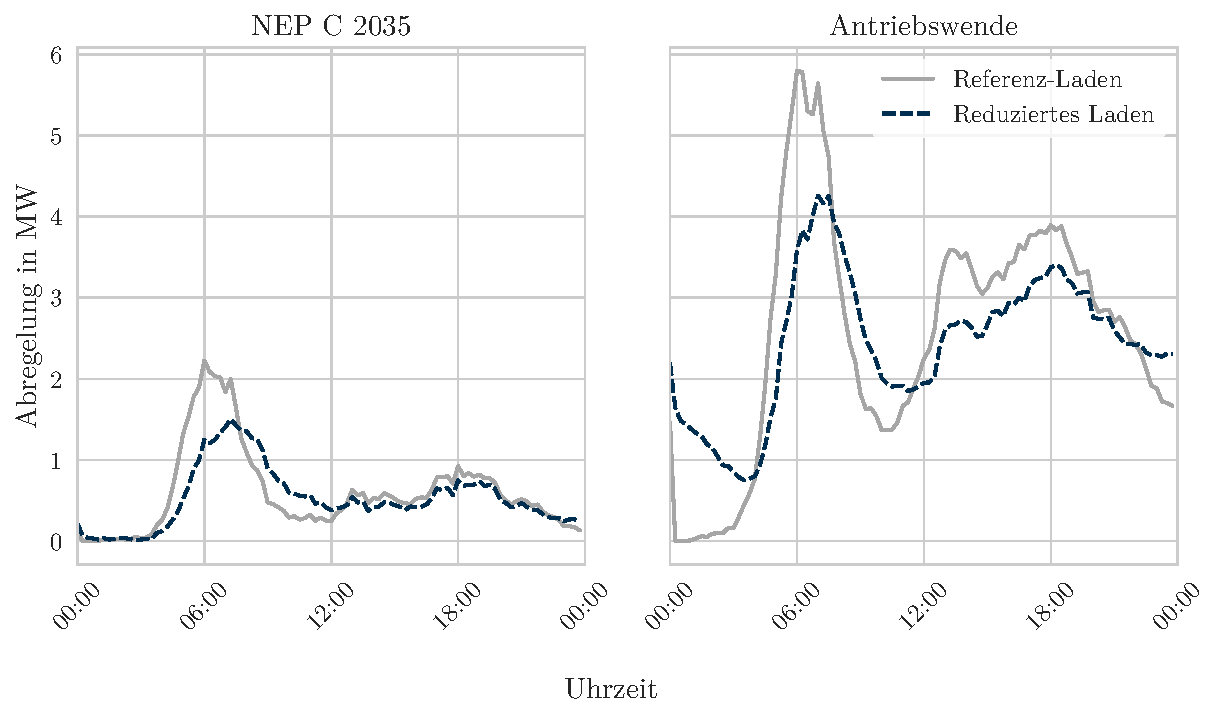
\includegraphics[width=\textwidth]{Bilder/176_load_curtailment_per_strategy}
    \caption{Durchschnittliche Abregelung von Lasten im NEP C~\num{2035} Szenario (links) und Antriebswende-Szenario (rechts) innerhalb von Woche~MIN im Netz \num{176}}\label{fig:176_load_curtailment_per_strategy}
\end{figure}

Das Residuallast-Laden kann den lastseitigne Abregelungsbedarf im Netz \(1056_{\text{PV}}\) noch deutlich stärker senken, als das reduzierte Laden.
In dem stark \gls{PV}-dominierten Netz \(1056_{\text{PV}}\) können im Antriebswende-Szenario sogar \SI{29.4}{\percent} der Abregelung durch die Residuallast-Ladestrategie verhindert werden, da die entsprechenden \gls{NS}-Netzkapazitäten für eine starke Verschiebung der Last gegeben sind.
Im Netz \(176_{\text{PV}}\)kommt es innerhalb der Hochzeit der \gls{PV}-Einspeisung bereits zu lastseitigen Abregelungen.
Da beim Residuallast-Laden viel Last in dieses Zeitfenster verschoben wird, erhöht sich der Abregelungsbedarf am frühen Nachmittag.
Aus diesem Grund fällt der Einfluss des Residuallast-Ladens auf den lastseitigen Abregelungsbedarf sehr gering aus, oder erhöht diesen sogar.\medskip

In Woche~MAX fällt der Abregelungsbedarf der Lasten beim Referenz-Laden im Netz \(176_{\text{PV}}\) mit \SIrange{115}{503}{\mwh} und im Netz \(1056_{\text{PV}}\) mit \SIrange{79}{149}{\mwh} erwartungsgemäß höher aus als in Woche~MIN.
Das Netz \(176_{\text{PV}}\) weist nach \autoref{fig:176_1056_cur_load_grid_week_B} ein sehr ähnliches Verhalten wie in Woche~MIN auf.
So kann vor allem in Szenarien mit einem niedrigeren Hochlauf an \gls{EPKW} Abregelung durch das reduzierte Laden verhindert werden.
Die beiden anderen Ladestrategien zeigen in der Regel nur einen minimalen Einfluss auf den Abregelungsbedarf.\medskip

Im NEP C~\num{2035} Szenario fällt der Einfluss der Lastverschiebung des Ladebedarfs auf die Residuallast aufgrund des insgesamt geringen Ladebedarfs begrenzt aus.
Aus diesem Grund wird viel Last in wenige Zeitschritte der Hochzeit der \gls{PV}-Einspeisung verschoben, weshalb die Gleichzeitigkeit besonders hoch ausfällt und es zu lastseitigem Abregelungsbedarf kommt.
Da hierbei teilweise auch Last aus Zeitschitten ohne Abregelungsbedarf nun in Zeitschritte mit Abregelungsbedarf verschoben wird, kommt es im NEP C~\num{2035} Szenario sogar zu einem erhöhten lastseitigen Abregelungsbedarf.
Durch die Zunahme des Einflusses auf die Residuallast mit einem steigenden Ladebedarf, fällt dieser Effekt in den anderen Szenarien schwächer aus.\medskip

Im Netz \(1056_{\text{PV}}\) kann hingegen der Abregelungsbedarf durch das Residuallast-Laden um bis zu \SI{10.5}{\percent} gesenkt werden.
Aufgrund der Zunahme der zur Verfügung stehenden flexiblen Leistung und Energie der \gls{EPKW} mit den Szenarien, kann auch immer stärker eine Glättung der Residuallast erreicht werden.
Hierdurch werden sowohl im Netz \(1056_{\text{PV}}\) als auch im Netz \(176_{\text{PV}}\) zunehmend immer mehr Zeitschritte zum Laden verwendet und die zeitliche Konzentration von Ladevorgängen innerhalb einiger weniger Zeitschritte nimmt im Vergleich ab, wodurch sich die Effektivität des Residuallast-Ladens mit den Szenarien graduell erhöht.\medskip

Lastseitig können im Netz \(1056_{\text{PV}}\) sowohl durch die Residuallast-Ladestrategie als auch durch das reduzierte Laden in erster Linie morgens große Mengen an Abregelung verhindert werden (vgl \autoref{fig:1056_fEE_load_diff}).
Zusätzlich kann durch die Residuallast-Ladestrategie auch am Abend ein signifikanter Anteil an Abregelung vermieden werden.
Zur Mittagszeit zeigt sich lastseitig ein erhöhter Abregelungsbedarf durch die Residuallast-Ladestrategie.
Es wird somit ein zu großer Anteil von Fahrzeugen innerhalb eines kurzen Zeitfensters geladen und vor allem die Betriebsmittel auf der \gls{NS}-Ebene überlastet.

\begin{figure}[H]
    \centering
    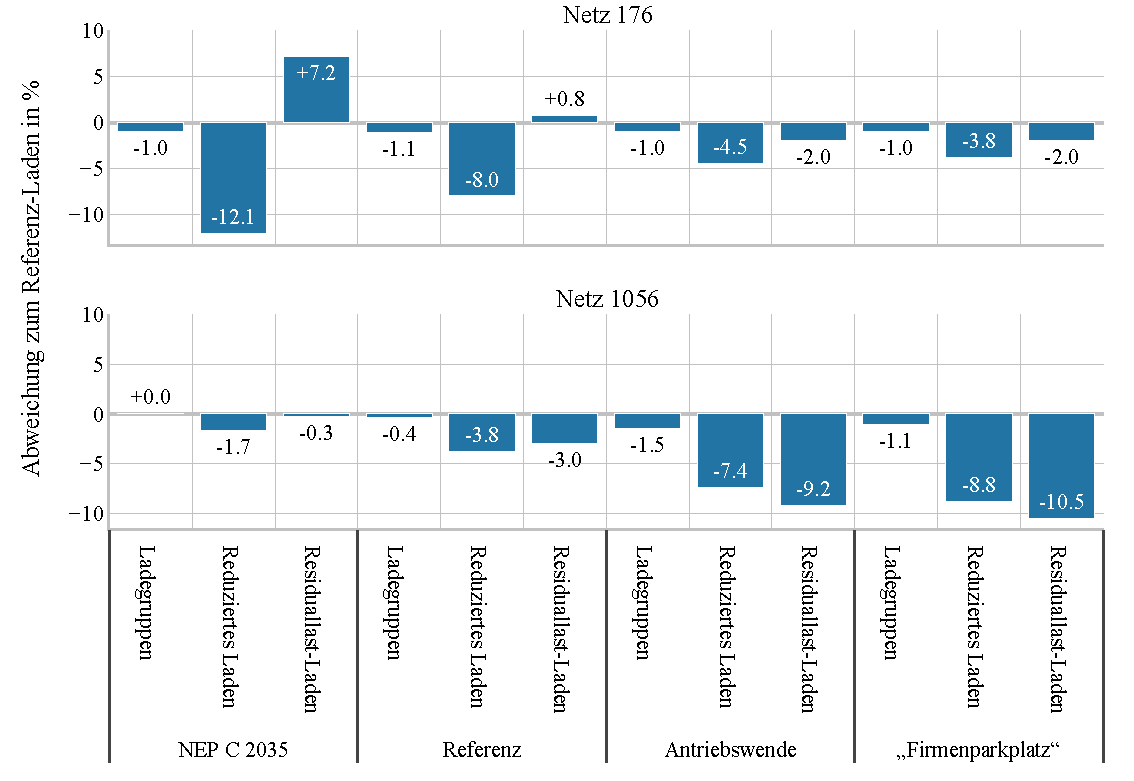
\includegraphics[width=\textwidth]{Bilder/176_1056_cur_load_grid_week_B}
    \caption[Prozentuale Veränderung des Abregelungsbedarfs von allen Lasten in Abhängigkeit von der Ladestrategie in Woche~MAX gegenüber dem Abregelungsbedarf für die Referenz-Ladestrategie je Szenario für die Netze \num{176} und \num{1056}]{Prozentuale Veränderung des Abregelungsbedarfs von allen Lasten in Abhängigkeit von der Ladestrategie in Woche~MAX gegenüber dem Abregelungsbedarf für die Referenz-Ladestrategie je Szenario für die Netze \(176_{\text{PV}}\) (oben) und \(1056_{\text{PV}}\) (unten)}\label{fig:176_1056_cur_load_grid_week_B}
\end{figure}

Bei den \gls{FEE} Anlagen zeigt sich, dass innerhalb von Woche~MAX in beiden \gls{PV}-dominierten Netzen keine Abregelung von \gls{FEE} Anlagen nötig ist, weshalb eine Betrachtung der Woche~MAX entfällt.
In Woche~MIN sinkt nach \autoref{tab:pv_dominated_week_a_fee_cur} der Abregelungsbedarf beim Referenz-Laden mit einem steigenden Hochlauf an \gls{EPKW}.
Dabei fällt auf, dass der Abregelungsbedarf von \gls{FEE} Anlagen in der \SzeFirmenparkplatz stärker abfällt als im Antriebswende-Szenario.
Dies lässt sich dadurch begründen, dass durch den höheren Anteil an Ladevorgängen im öffentlichen Raum und \zH nach \autoref{fig:example_load_profile} mehr Ladevorgänge in den zeitlichen Bereich hoher Einspeisung am frühen Nachmittag fallen und somit ein besserer Ausgleich zwischen Angebot und Nachfrage entsteht.
Im Antriebswende-Szenario finden beim Referenz-Laden hingegen deutlich mehr Ladevorgänge am Morgen statt.
In dieser Zeit kommt es zu keiner hohen Einspeisung durch \glspl{PVA}.
Innerhalb von \gls{NS}-Netzen mit einem hohen Anteil an Ladevorgängen \zH befinden sich oft auch viele \glspl{PVA}.
Da in der \SzeFirmenparkplatz mehr Ladevorgänge \zH stattfinden, wird der Abregelungsbedarf von \gls{FEE} Anlagen somit gesenkt.

{
\renewcommand{\arraystretch}{1.2}% grßerer Zeilenabstand
\sisetup{range-phrase=~{--}~}% Gedankenstrich statt "bis" bei SIrange
\begin{table}[H]
	\begin{center}
		\caption{Abregelungsbedarf von fEE Anlagen in den PV-dominierten Netzen je Szenario für die Referenz-Ladestrategie in Woche~MIN}
		\begin{tabu} to 0.6\textwidth {X[1.5] X[1, r] X[1, r]}
			\toprule
			Abregelung in   \si{\mwh}    & Netz \(176_{\text{PV}}\) & Netz \(1056_{\text{PV}}\) \\ \midrule
			NEP C~\num{2035}             & \num{20.5}     & \num{88.8}      \\
			Referenz                     & \num{18.4}     & \num{84.3}      \\
			Antriebswende                & \num{15.8}     & \num{76.0}      \\
			\glqq Firmenparkplatz\grqq{} & \num{15.1}     & \num{73.6}      \\ \bottomrule
		\end{tabu}
		\label{tab:pv_dominated_week_a_fee_cur}
	\end{center}
	\vspace{-3mm}%Put here to reduce too much white space after your table
\end{table}
}

\autoref{fig:176_1056_cur_fee_grid_week_A} zeigt die prozentuale Veränderung des Abregelungsbedarfs von \gls{FEE} Anlagen in Abhängigkeit von der Ladestrategie.
So kann der Abregelungsbedarf durch die Residuallast-Ladestrategie im Netz \(1056_{\text{PV}}\) um bis zu \SI{10.7}{\percent} und im Netz \(176_{\text{PV}}\) aufgrund des geringeren Verhältnisses zwischen Einspeisung und Ladebedarf sogar um bis zu \SI{20.3}{\percent} gesenkt werden.
Da im Antriebswende-Szenario deutlich mehr flexible Leistung und Energie durch \gls{EPKW} zur Verfügung steht als in den anderen Szenarien, kann innerhalb dieses Szenarios die stärkste Reduktion erreicht werden.
Weiterhin finden gegenüber der \SzeFirmenparkplatz mehr flexible Ladevorgänge (vgl. \autoref{tab:ChargingShare}) statt.
Da innerhalb der Standzeiten des \UC \Firmeparkplatz in der Regel auch die Hochzeiten der Einspeisung von \glspl{PVA} liegen, bietet dieses Szenario in beiden Netzen ein um mehr als \SI{30}{\percent} größeres Einsparpotential beim Abregelungsbedarf von \gls{FEE} Anlagen.


\begin{figure}[H]
    \centering
    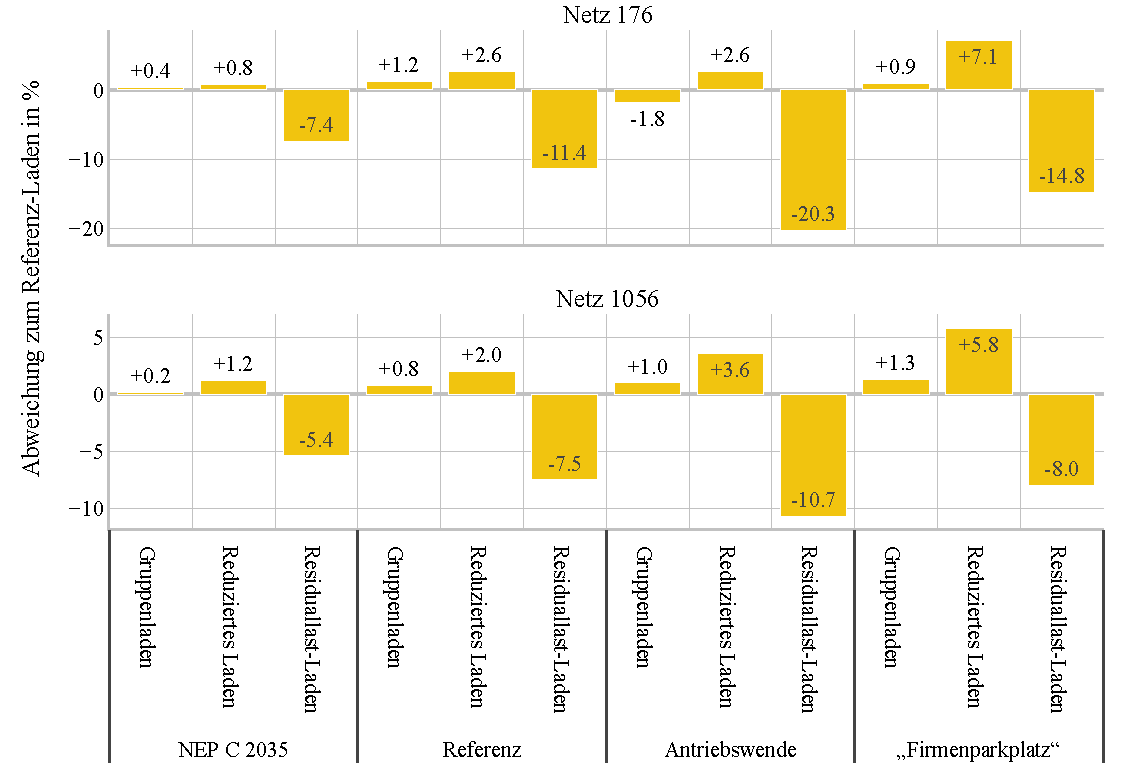
\includegraphics[width=\textwidth]{Bilder/176_1056_cur_fee_grid_week_A}
    \caption{Prozentuale Veränderung des Abregelungsbedarf von fEE Anlagen in Abhängigkeit von der Ladestrategie in Woche A gegenüber dem Abregelungsbedarf für die Referenz-Ladestrategie je Szenario für die Netze \num{176} (oben) und \num{1056} (unten)}\label{fig:176_1056_cur_fee_grid_week_A}
\end{figure}

In \autoref{fig:1056_fEE_load_diff} findet sich die durchschnittliche Abregelung von \gls{FEE} Anlagen und Lasten (oben) in Abhängigkeit von der Uhrzeit in Woche~MIN für das Referenz-Laden im Netz \(1056_{\text{PV}}\).
Zusätzlich ist die Differenz zwischen den Ladestrategien und dem Referenz-Laden (unten) dargestellt, wobei negative Werte einen geringeren Abregelungsbedarf signalisieren.
Dabei zeigt sich, dass in dem stark \gls{PV}-dominierten Netz \(1056_{\text{PV}}\) Abregelung von \gls{FEE} Anlagen ausschließlich tagsüber und vor allem am frühen Nachmittag nötig ist.
Demgegenüber treten die lastseitigen Abregelungsspitzen hierzu versetzt morgens und abends auf.
Durch die Residuallast-Ladestrategie kann der Abregelungsbedarf von \gls{FEE} Anlagen vor allem in Zeiten von Spitzeneinspeisung gesenkt werden.\medskip

In den beiden \gls{PV}-dominierten Netzen kommt es insgesamt zu einer Abnahme der Effizienz erzeugerseitige Abregelung zu verhindern, mit jeder zusätzlich verschobenen Kilowattstunde.
So beträgt im Netz \(1056_{\text{PV}}\) im NEP C~\num{2035} Szenario das Verhältnis zwischen der Einsparung erzeugerseitiger Abregelung aufgrund des Residuallast-Ladens gegenüber dem Referenzladen und dem flexibilsierbaren Ladebedarf noch \SI{-6.1}{\percent}.
Mit Hilfe dieser Kennzahl soll die Effizienz des Residuallast-Ladens zwischen den \gls{MS}-Netzen vergleichbar gemachtw erden, wobei negative Werte für eine Reduktion des Abregelungsbedarfs von \gls{FEE} Anlagen stehen.
Im Antriebswende-Szenario sinkt dieser Wert auf \SI{-3.1}{\percent}.
Für das Netz \(176_{\text{PV}}\) liegen beide Werte mit \SI{-0.7}{\percent} bzw. \SI{-0.5}{\percent} deutlich niedriger, da der Ladebedarf in diesem Netz höher und der erzeugerseitige Abregelungsbedarf geringer ausfällt.
Da hauptsächlich Ladevorgänge des \UCs \Firmeparkplatz in die für erzeugerseitige Abreglung relevanten Zeitfenster verschoben werden, fällt dieser Wert in den beiden Netzen mit \SIrange[range-phrase=~bzw.~]{-2.4}{-0.3}{\percent} in der \SzeFirmenparkplatz noch geringer aus.
Eine vollständige Aufstellung ist im Anhang in \autoref{tab:ratio_cur_demand} dargestellt.

\begin{figure}[H]
    \centering
    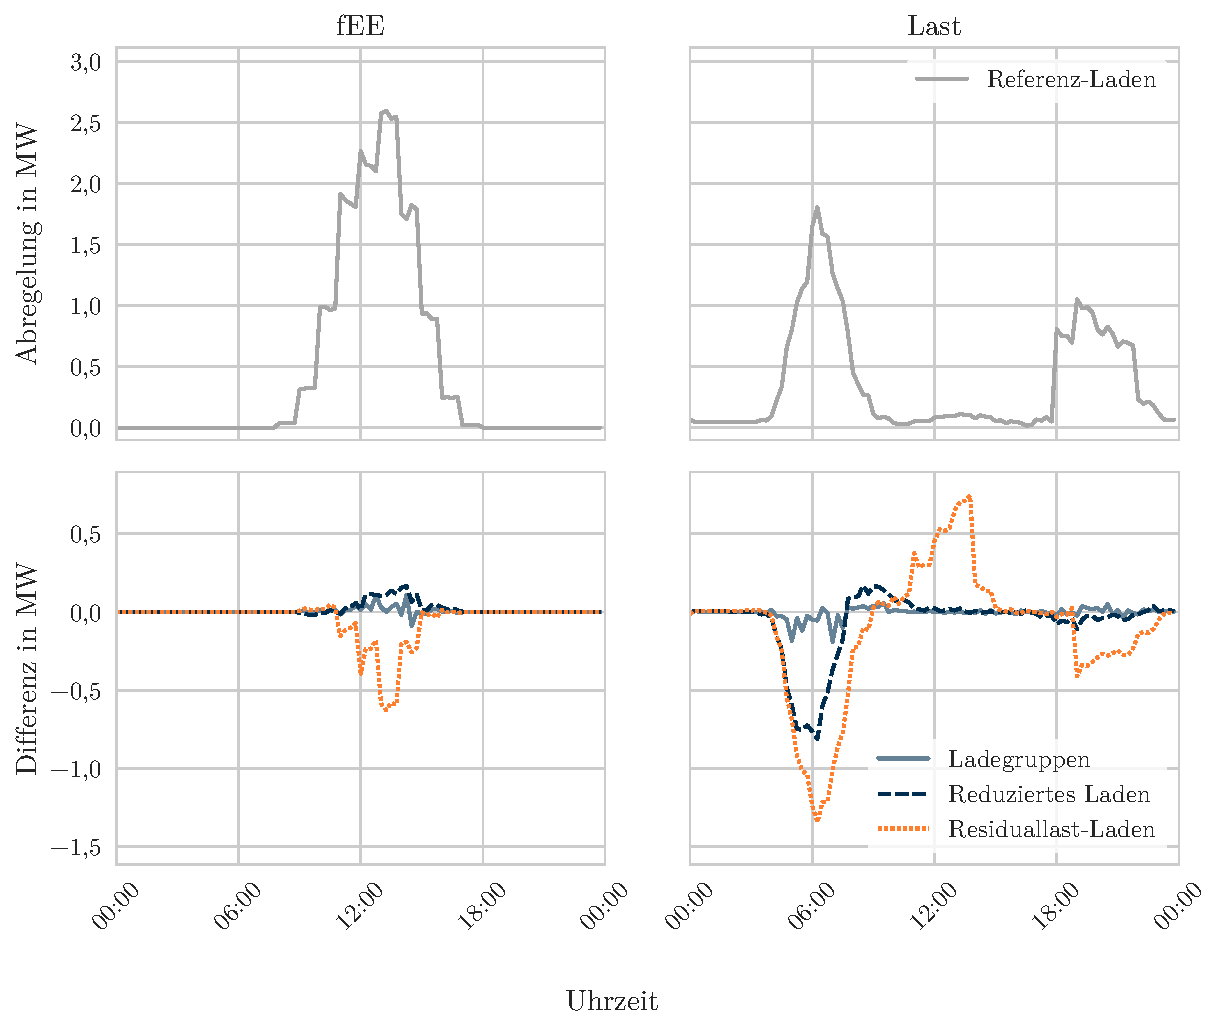
\includegraphics[width=\textwidth]{Bilder/1056_fEE_load_diff}
    \caption{Durchschnittliche Abregelung von fEE Anlagen (oben links) und Lasten (oben rechts) innerhalb von Woche A und die durchschnittliche Differenz des Abregelungsbedarfs der Ladestrategien gegenüber dem Referenz-Laden für fEE Anlagen (unten links) und Lasten (unten rechts) im Antriebswende-Szenario im Netz \num{1056}}\label{fig:1056_fEE_load_diff}
\end{figure}

Beim den Ladegruppen und beim reduzierten Laden kommt es zu einem erhöhten Abregelunsgebedarf von \gls{FEE} Anlagen zur Mittagszeit.
Nach \autoref{fig:example_load_profile} werden ab der Mittagszeit viele Fahrzeuge \zH geladen.
Durch die präventiven Ladestrategien kommt es dazu, dass der Ladebedarf für den \UC \zH in dieser Zeit im Durchschnitt geringer ausfällt als beim Referenz-Laden, da die Ladevorgänge zeitlich gestreckt werden.
Da in \gls{NS}-Netzen mit einem hohen Anteil an Ladevorgängen des \UCs \zH in der Regel auch viele \glspl{PVA} angeschlossen sind, kommt es insgesamt zu einer Erhöhung des erzeugerseitigen Abregelungsbedarfs.
Vor allem beim reduzierten Laden spiegelt sich dies in dem Absinken der Residuallast in Zeiten von Spitzeneinspeisung (vgl. \autoref{fig:residual_load}) wider.


\paragraph{Fazit:}

Der Hochlauf der Elektromobilität gestaltet sich in den beiden betrachteten \gls{PV}-dominierten Netzen stark unterschiedlich.
Im Falle des Netzes \(176_{\text{PV}}\) werden einzelne \gls{NS}-Netze so stark überlastet, dass ein großer Anteil des Ladebedarfs der \gls{EPKW} abgeregelt werden muss.
Demgegenüber fällt der Abregelungsbedarf des Ladebedarfs im Netz \(1056_{\text{PV}}\) deutlich moderater aus. \medskip

Die Ladegruppen zeigen insgesamt eine sehr geringe Wirksamkeit auf den Abregelungsbedarf.
Für die anderen Ladestrategien ergeben sich aus der unterschiedlich starken Überlastung der beiden Netze starke Potentialunterschiede in der Wirksamkeit.
So kann das reduzierte Laden weitgehend den lastseitigen Abregelungsbedarf um einen signifikanten Anteil senken.
Dabei zeigt sich jedoch, dass das Einsparpotential mit einer zunehmenden Überlastung der \gls{NS}-Netze abnimmt, da es zunehmend auch nachts und mittags zu Abregelungen des Ladebedarfs kommt und dieser zeitlich nur noch verschoben aber nicht verhindert wird.
Das aktive Residuallast-Laden kann gegenüber den präventiven Ladestrategien weitere lastseitige Abregelung verhindern, wenn die entsprechenden \gls{NS}-Netzkapazitäten gegeben sind oder/und die Erzeugerkapazitäten in den gleichen \gls{NS}-Netzen liegen, in denen auch der Ladebedarf anfällt.\medskip

Es zeigt sich, dass nur durch die aktive Verschiebung des Ladebedarfs in die Hochzeiten der Einspeisung von \gls{FEE} Anlagen bei der Residuallast-Ladestrategie der erzeugerseitige Abregelungsbedarf reduziert werden kann.
Allerdings wird in der Regel so viel Ladebedarf in die Hochzeiten der Einspeisung verschoben, dass es aufgrund der hohen Gleichzeitigkeit zu einer erhöhten Abregelung des Ladebedarfs kommt.
Das Potential, den lastseitigen und erzeugerseitigen Abregelungsbedarf zu senken, wird auf diese Weise nicht voll ausgeschöpft.
Es empfiehlt sich neben dem Optimierungsansatz der Residuallast-Glättung vor allem auch die Belastungsgrenzen der \gls{NS}-Betriebsmittel zu beachten.
Auf diese Weise würde mehr Ladebedarf in Zeiten einer schwächeren Einspeisung verschoben werden und voraussichtlich könnte der Abregelungsbedarf last- und einspeiseseitig weiter gesenkt werden.
Die präventiven Ladestrategien führen demgegenüber zu einer Erhöhung des erzeugerseitigen Abregelungsbedarfs, da der Ladebedarf am frühen Nachmittag reduziert wird und somit nicht mehr in die Hochzeiten der Einspeisung der \glspl{PVA} fällt.


\subsubsection{Wind-dominierte Netze}\label{chap:wind_cur_results}

Die Wind-dominierten Netze \(1690_{\text{W}}\) und \(1811_{\text{W}}\) weisen gegenüber den \gls{PV}-dominierten Netzen eine deutlich größere Differenz zwischen Erzeugung und Bedarf auf.
So liegt das Verhältnis zwischen der Einspeisung von \gls{FEE} Anlagen und dem Ladebedarf von \gls{EPKW} nach \autoref{tab:wind_dominated_week_a_char} und \autoref{tab:wind_dominated_epkw_demand} im Antriebswende-Szenario in Woche~MIN im Netz \(1811_{\text{W}}\) bei etwa \(19:1\) und im Netz \(1690_{\text{W}}\) sogar bei etwa \(33:1\).
Hieraus folgt gegenüber den \gls{PV}-dominierten Netzen ein deutlich reduziertes Potential die Residuallast und den Abregelungsbedarf von \gls{FEE} Anlagen zu beeinflussen.

{
\renewcommand{\arraystretch}{1.2}% grßerer Zeilenabstand
\sisetup{range-phrase=~{--}~}% Gedankenstrich statt "bis" bei SIrange
\begin{table}[H]
	\begin{center}
		\caption{Einspeisung von fEE und nicht-fEE sowie der Bedarf von sonstigen Lasten in den Wind-dominierten Netzen in Woche~MIN}
		\begin{tabu} to 0.6\textwidth {X[1.7] X[1, r] X[1, r]}
			\toprule
			Angaben in \si{\mwh}	& Netz \(1690_{\text{W}}\) & Netz \(1811_{\text{W}}\) \\ \midrule
			Einspeisung fEE      	& \num{11971.2}   & \num{8966.5}    \\
			Einspeisung Sonstige 	& \num{4808.5}    & \num{2541.0}    \\
			Bedarf Sonstige     	& \num{1442.8}    & \num{1599.2}    \\ \bottomrule
		\end{tabu}
		\label{tab:wind_dominated_week_a_char}
	\end{center}
	\vspace{-3mm}%Put here to reduce too much white space after your table
\end{table}
}

{
\renewcommand{\arraystretch}{1.2}% grßerer Zeilenabstand
\sisetup{range-phrase=~{--}~}% Gedankenstrich statt "bis" bei SIrange
\begin{table}[H]
	\begin{center}
		\caption{Ladebedarf der E-Pkw in den Wind-dominierten Netzen je Szenario}
		\begin{tabu} to 0.6\textwidth {X[1.5] X[1, r] X[1, r]}
			\toprule
			Ladebedarf in   \si{\mwh}    & Netz \num{1690} & Netz \num{1811} \\ \midrule
			NEP C~\num{2035}             & \num{111.9}     & \num{135.2}     \\
			Referenz                     & \num{199.2}     & \num{244.6}     \\
			Antriebswende                & \num{361.5}     & \num{465.3}     \\
			\glqq Firmenparkplatz\grqq{} & \num{363.0}     & \num{459.9}     \\ \bottomrule
		\end{tabu}
		\label{tab:wind_dominated_epkw_demand}
	\end{center}
	\vspace{-3mm}%Put here to reduce too much white space after your table
\end{table}
}

In \autoref{tab:wind_dominated_week_a_epkw_cur} findet sich der Abregelungsbedarf des Ladebedarfs von \gls{EPKW} in den Wind-dominierten Netzen für die Referenz-Ladestrategie in Woche~MIN und in \autoref{tab:wind_dominated_week_a_load_cur} ergänzend der Abregelungsbedarf für die sonstigen Lasten.
Auch bei den Wind-dominierten Netzen kommt es zu einer Zunahme des Abregelungsbedarfs mit dem Hochlauf der \gls{EPKW}.
Da die Windkraft-Erzeugerkapazitäten in der Regel direkt in der \gls{MS}-Ebene angeschlossen werden und auch absolut eine größer Erzeugerleistung in den Wind-dominierten Netzen installiert ist (vgl. \autoref{fig:bar_representatives}), ist die \gls{MS}-Ebene in den Wind-dominierten Netzen auf höhere Lasten ausgelegt als in den \gls{PV}-dominierten Netzen.
Der lastseitige Abregelungsbedarf beschränkt sich deshalb beinahe vollständig auf die \gls{NS}-Ebene.
Das Netz \(1690_{\text{W}}\) zeigt vergleichbar zum Netz \(176_{\text{PV}}\) einen höheren Abregelungsbedarf in der \SzeFirmenparkplatz gegenüber dem Antriebswende-Szenario.
So zeigt auch das Netz \(1690_{\text{W}}\) die Tendenz, dass vor allem \gls{NS}-Netze mit einem hohen Anteil an Ladeinfrastruktur \zH stark ausgelastet sind und der zusätzliche Ladebedarf \zH in der \SzeFirmenparkplatz somit den Abregelungsbedarf erhöht.
Zusätzlich fällt der Ladebedarf insgesamt in der \SzeFirmenparkplatz höher aus, als im Antriebswende-Szenario.

{
\renewcommand{\arraystretch}{1.2}% grßerer Zeilenabstand
\sisetup{range-phrase=~{--}~}% Gedankenstrich statt "bis" bei SIrange
\begin{table}[H]
	\begin{center}
		\caption{Abregelungsbedarf des Ladebedarfs von E-Pkw in den Wind-dominierten Netzen je Szenario für die Referenz-Ladestrategie in Woche A}
		\begin{tabu} to 0.6\textwidth {X[1.5] X[1, r] X[1, r]}
			\toprule
			Abregelung in   \si{\mwh}    & Netz \num{1690} & Netz \num{1811} \\ \midrule
			NEP C~\num{2035}             & \num{2.5}       & \num{1.6}       \\
			Referenz                     & \num{7.8}       & \num{7.1}       \\
			Antriebswende                & \num{18.4}      & \num{20.4}      \\
			\glqq Firmenparkplatz\grqq{} & \num{20.1}      & \num{17.7}      \\ \bottomrule
		\end{tabu}
		\label{tab:wind_dominated_week_a_epkw_cur}
	\end{center}
	\vspace{-3mm}%Put here to reduce too much white space after your table
\end{table}
}

{
\renewcommand{\arraystretch}{1.2}% grßerer Zeilenabstand
\sisetup{range-phrase=~{--}~}% Gedankenstrich statt "bis" bei SIrange
\begin{table}[H]
	\begin{center}
		\caption{Abregelungsbedarf der sonstigen Lasten in den Wind-dominierten Netzen je Szenario für die Referenz-Ladestrategie in Woche A}
		\begin{tabu} to 0.6\textwidth {X[1.5] X[1, r] X[1, r]}
			\toprule
			Abregelung in   \si{\mwh}    & Netz \num{1690} & Netz \num{1811} \\ \midrule
			NEP C~\num{2035}             & \num{3.5}       & \num{2.6}       \\
			Referenz                     & \num{4.4}       & \num{3.7}       \\
			Antriebswende                & \num{7.0}       & \num{6.3}       \\
			\glqq Firmenparkplatz\grqq{} & \num{7.0}       & \num{6.3}       \\ \bottomrule
		\end{tabu}
		\label{tab:wind_dominated_week_a_load_cur}
	\end{center}
	\vspace{-3mm}%Put here to reduce too much white space after your table
\end{table}
}

In den Wind-dominierten Netzen kann der lastseitige Abregelungsbedarf nach \autoref{fig:1690_1811_cur_load_grid_week_A} und \autoref{fig:1690_1811_cur_load_grid_week_B} in beinahe allen Fällen durch die Ladestrategien gesenkt werden.
Es zeigt sich erneut, dass die Ladegruppen nur einen geringen Einfluss auf den lastseitigen Abregelungsbedarf aufweist.
Das reduzierte Laden erweist sich im Gegensatz zu den \gls{PV}-dominierten Netzen in allen Fällen effektiver als das Residuallast-Laden, um den lastseitigen Abregelungsbedarf zu senken.\medskip

\begin{figure}[H]
    \centering
    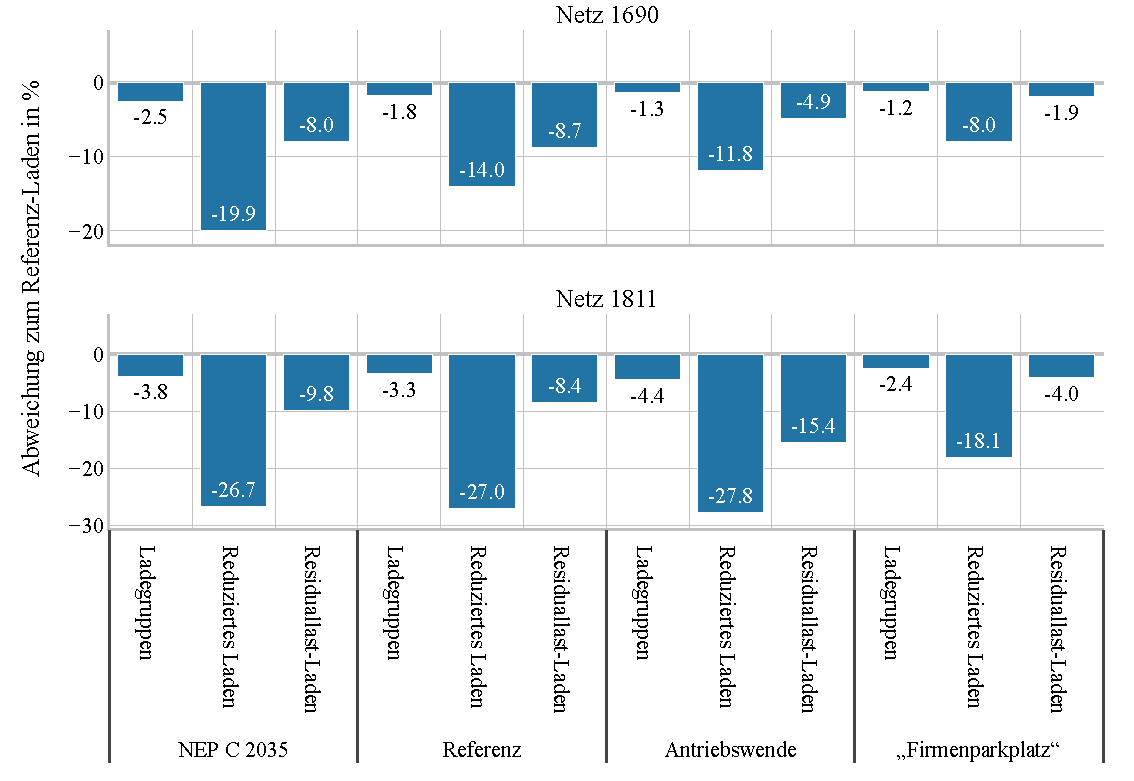
\includegraphics[width=\textwidth]{Bilder/1690_1811_cur_load_grid_week_A}
    \caption[Prozentuale Veränderung des Abregelungsbedarfs von allen Lasten in Abhängigkeit von der Ladestrategie in Woche~MIN gegenüber dem Abregelungsbedarf für die Referenz-Ladestrategie je Szenario für die Netze \num{1690} und \num{1811}]{Prozentuale Veränderung des Abregelungsbedarfs von allen Lasten in Abhängigkeit von der Ladestrategie in Woche~MIN gegenüber dem Abregelungsbedarf für die Referenz-Ladestrategie je Szenario für die Netze \(1690_{\text{W}}\) (oben) und \(1811_{\text{W}}\) (unten)}\label{fig:1690_1811_cur_load_grid_week_A}
\end{figure}

In Woche~MIN kann im Netz \(1811_{\text{W}}\) durch das reduzierte Laden noch eine annähernd konstante Senkungswirkung der lastseitigen Abregelung in den unterschiedlichen Szenarien erreicht werden.
Demgegenüber kann in Woche~MAX und und im Netz \(1690_{\text{W}}\) eine Abnahme des Einsparpotentials an lastseitiger Abregelung mit einem zunehmenden Hochlauf an \gls{EPKW} festgestellt werden.
Die beiden Netze Verhalten sich hierbei ähnlich wie das \gls{PV}-dominierte Netz \(176_{\text{PV}}\).
Im Unterschied zu dem Netz \(176_{\text{PV}}\) kommt es in den Wind-dominierten Netzen nachts in der Regel nicht zu einer lastseitigen Abregelung (vgl. \autoref{fig:1690_fEE_load_diff} (oben rechts)).
Hierdurch kann durch das reduzierte Laden Ladebedarf erfolgreich in die Nacht verschoben werden, ohne den Abregelungsbedarf zu erhöhen.
In den Szenarien mit einem geringeren Hochlauf an \gls{EPKW} kommt es beim Referenz-Laden in erster Linie zur Abregelung von Last am Morgen und am Abend.
Bei einem höheren Hochlauf an \gls{EPKW} kommt es zusätzlich zur lastseitigen Abregelungen zur Mittagszeit und am frühen Nachmittag.
Durch das reduzierte Laden kann in diesen Fällen Abregelungsbedarf nur mit nachlassendem Erfolg verhindert werden, da vermehrt Abregelungsbedarf nur noch vom Vormittag auf den frühen Nachmittag verschoben wird.
Das Netz \(1811_{\text{W}}\) besitzt bei einem moderat erhöhten Ladebedarf gegenüber dem Netz \(1690_{\text{W}}\) eine deutlich höhere Anzahl an \gls{NS}-Netzen weshalb die einzelnen \gls{NS}-Netze meist geringer belastet werden.
Hierdurch entsteht dieser Trend im Netz \(1811_{\text{W}}\) erst in den erhöhten Lastfällen der Woche~MAX.

\begin{figure}[H]
    \centering
    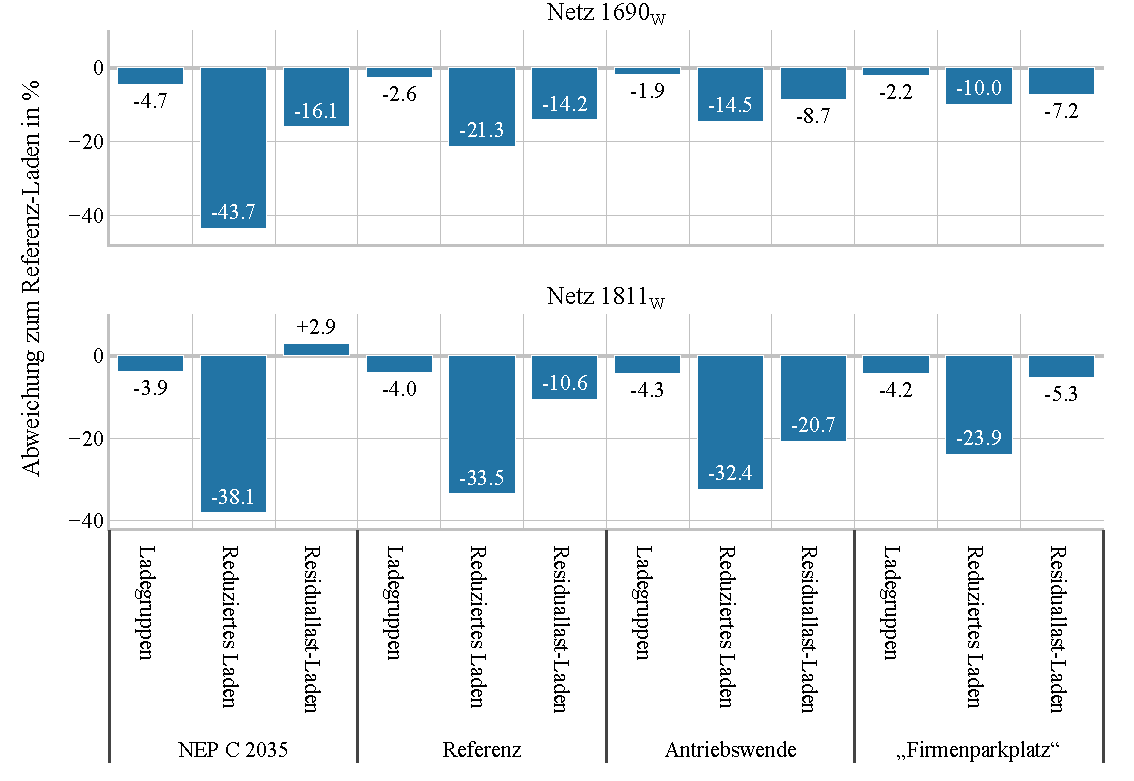
\includegraphics[width=\textwidth]{Bilder/1690_1811_cur_load_grid_week_B}
    \caption[Prozentuale Veränderung des Abregelungsbedarfs von allen Lasten in Abhängigkeit von der Ladestrategie in Woche~MAX gegenüber dem Abregelungsbedarf für die Referenz-Ladestrategie je Szenario für die Netze \num{1690} und \num{1811}]{Prozentuale Veränderung des Abregelungsbedarfs von allen Lasten in Abhängigkeit von der Ladestrategie in Woche~MAX gegenüber dem Abregelungsbedarf für die Referenz-Ladestrategie je Szenario für die Netze \(1690_{\text{W}}\) (oben) und \(1811_{\text{W}}\) (unten)}\label{fig:1690_1811_cur_load_grid_week_B}
\end{figure}

Der Vorteil des reduzierten Ladens gegenüber dem Residuallast-Laden entsteht, weil es auch in den Wind-dominierten Netzen einen gewissen Anteil an \gls{PV}-Erzeugerkapazitäten gibt.
Dies führt dazu, dass beim Residuallast-Laden ein großer Anteil an Ladevorgängen in die Hochzeit der \gls{PV}-Einspeisung zum Mittag und frühen Nachmittag verschoben wird.
Da die \gls{NS}-Netze in diesem Zeitraum, wie zuvor beschrieben, bereits stark belastet sind, führt diese zusätzliche Last zu einem erhöhten Abregelungsbedarf, welches in \autoref{fig:1690_fEE_load_diff} (unten rechts) zu erkennen ist.
Weiterhin ist aufgrund des hohen Verhältnisses zwischen Einspeisung und Ladebedarf in den Wind-dominierten Netzen der Einfluss des Ladebedarfs auf die Residuallast gering.
Hierdurch tritt eine besonders starke zeitliche Konzentration der Ladevorgänge in den Wind-dominierten Netzen beim Residuallast-Laden auf, was den Abregelungsbedarf weiter erhöht.

{
\renewcommand{\arraystretch}{1.2}% grßerer Zeilenabstand
\sisetup{range-phrase=~{--}~}% Gedankenstrich statt "bis" bei SIrange
\begin{table}[H]
	\begin{center}
		\caption{Abregelungsbedarf von fEE Anlagen in den Wind-dominierten Netzen je Szenario für die Referenz-Ladestrategie in Woche~MIN}
		\begin{tabu} to 0.6\textwidth {X[1.5] X[1, r] X[1, r]}
			\toprule
			Abregelung in   \si{\mwh}    & Netz \num{1690} & Netz \num{1811} \\ \midrule
			NEP C~\num{2035}             & \num{319.1}     & \num{0.0}       \\
			Referenz                     & \num{315.2}     & \num{0.0}       \\
			Antriebswende                & \num{312.3}     & \num{0.0}       \\
			\glqq Firmenparkplatz\grqq{} & \num{311.9}     & \num{0.0}       \\ \bottomrule
		\end{tabu}
		\label{tab:wind_dominated_week_a_fee_cur}
	\end{center}
	\vspace{-3mm}%Put here to reduce too much white space after your table
\end{table}
}

Bei der Abregelung von \gls{FEE} Anlagen in den Wind-dominierten Netzen zeigt sich, dass keine Abregelung in Woche~MAX nötig ist.
Weiterhin ist im Netz \(1811_{\text{W}}\) nach \autoref{tab:wind_dominated_week_a_fee_cur} auch in Woche~MIN keine Abregelung notwendig, weshalb der Fokus auf der Betrachtungen der Woche~MIN im Netz \(1690_{\text{W}}\) liegt.
Im Netz \(1690_{\text{W}}\) zeigt sich vergleichbar zu den \gls{PV}-dominierten Netzen eine Abnahme des Abregelungsbedarfs mit dem Hochlauf an \gls{EPKW}.\medskip

Die Ladestrategien zeigen nach \autoref{fig:1690_cur_fee_grid_week_A} insgesamt einen extrem geringen Einfluss auf den erzeugungsseitigen Abregelungsbedarf von maximal \SI{1}{\percent}.
Dies liegt zum einen darin begründet, dass das Verhältnis aus Erzeugung zu Ladebedarf im Netz \(1690_{\text{W}}\) extrem hoch ausfällt und zum anderen darin, dass in Woche~MIN in \SI{83}{\percent} der Zeitschritte eine erzeugerseitige Abregelung nötig ist, welches sich in \autoref{fig:1690_fEE_load_diff} darin äußert, dass die durchschnittliche Abregelung der \gls{FEE} Anlagen (oben links) nie auf Null sinkt.
Hierdurch ergibt sich auf der einen Seite, dass das Potential zur Einflussnahme sehr gering ausfällt und auf der anderen Seite, dass auch erzeugerseitige Abregelung nur zeitlich verschoben wird.
So wird beispielsweise beim reduzierten Laden vor allem nachts Abregelung von Windkraftanlagen verhindert.
Dafür kommt es morgens und nachmittags zu einem erhöhten Abregelungsbedarf, da der Ladebedarf in diesen Zeitfenstern stark reduziert wird.
Insgesamt wird der Abregelungsbedarf hierdurch leicht erhöht.

\begin{figure}[H]
    \centering
    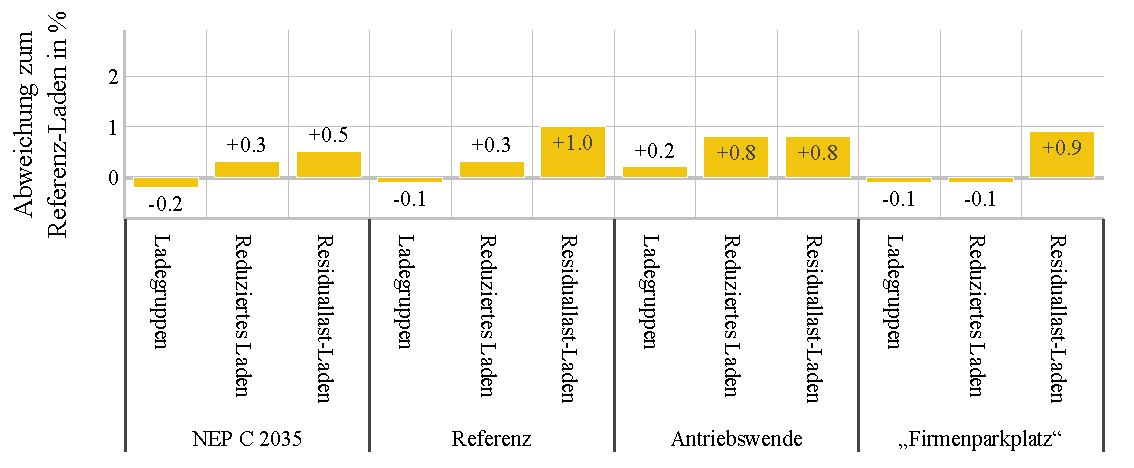
\includegraphics[width=\textwidth]{Bilder/1690_cur_fee_grid_week_A}
    \caption[Prozentuale Veränderung des Abregelungsbedarfs von fEE Anlagen in Abhängigkeit von der Ladestrategie in Woche~MIN gegenüber dem Abregelungsbedarf für die Referenz-Ladestrategie je Szenario für das Netze \num{1690}]{Prozentuale Veränderung des Abregelungsbedarfs von fEE Anlagen in Abhängigkeit von der Ladestrategie in Woche~MIN gegenüber dem Abregelungsbedarf für die Referenz-Ladestrategie je Szenario für das Netze \(1690_{\text{W}}\)}\label{fig:1690_cur_fee_grid_week_A}
\end{figure}

Im Gegensatz zu den \gls{PV}-dominierten Netzen zeigt sich, dass der erzeugerseitige Abregelungsbedarf durch die Residuallast-Ladestrategie nicht abgesenkt werden kann und sich sogar deutlicher erhöht als bei den präventiven Ladestrategien.
Hierbei kommt es zu einer ungünstigen zeitlichen und lokalen Konzentration von Ladevorgängen.
So kann der erzeugerseitige Abregelungsbedarf nach \autoref{fig:1690_fEE_load_diff} am frühen Nachmittag (grüner Bereich) gesenkt werden, während sich der Abregelungsbedarf anschließend (roter Bereich) erhöht.
In dem grünen Bereich kommt es in erster Linie zu einer Anhebung des Ladebedafs des \UC \Firmeparkplatzdot, da aufgrund des \gls{PV}-Anteils im \gls{MS}-Netz in der Regel die geringste Residuallast während der üblichen Standzeiten des \UCs \Firmeparkplatz vorherrscht.
Weiterhin sind die Standzeiten des \UC \Firmeparkplatz in der Regel kürzer als \zH (vgl. \autoref{tab:StandingTime}), weshalb die Priorität dieser Ladevorgänge bei der Vergabe der Ladezeitfenster nach \autoref{chap:theo_strategies} höher ausfällt.
Innerhalb der \gls{NS}-Netze, in denen viele Ladevorgänge des \UC \Firmeparkplatz stattfinden, befinden sich im Netz \(1690_{\text{W}}\) nur wenige \glspl{PVA}.
Aus diesem Grund kommt es zwar insgesamt zu einer Reduktion des erzeugerseitigen Abregelungsbedarfs innerhalb dieses Zeitfensters, aber der vermiedene Abregelungsbedarf fällt im Verhältnis zum aufgewendeten Ladebedarf gering aus.
Zusätzlich erhöht sich der lastseitige Abregelungsbedar, was die Effizienz der Ladestrategie weiter senkt.

\begin{figure}[H]
    \centering
    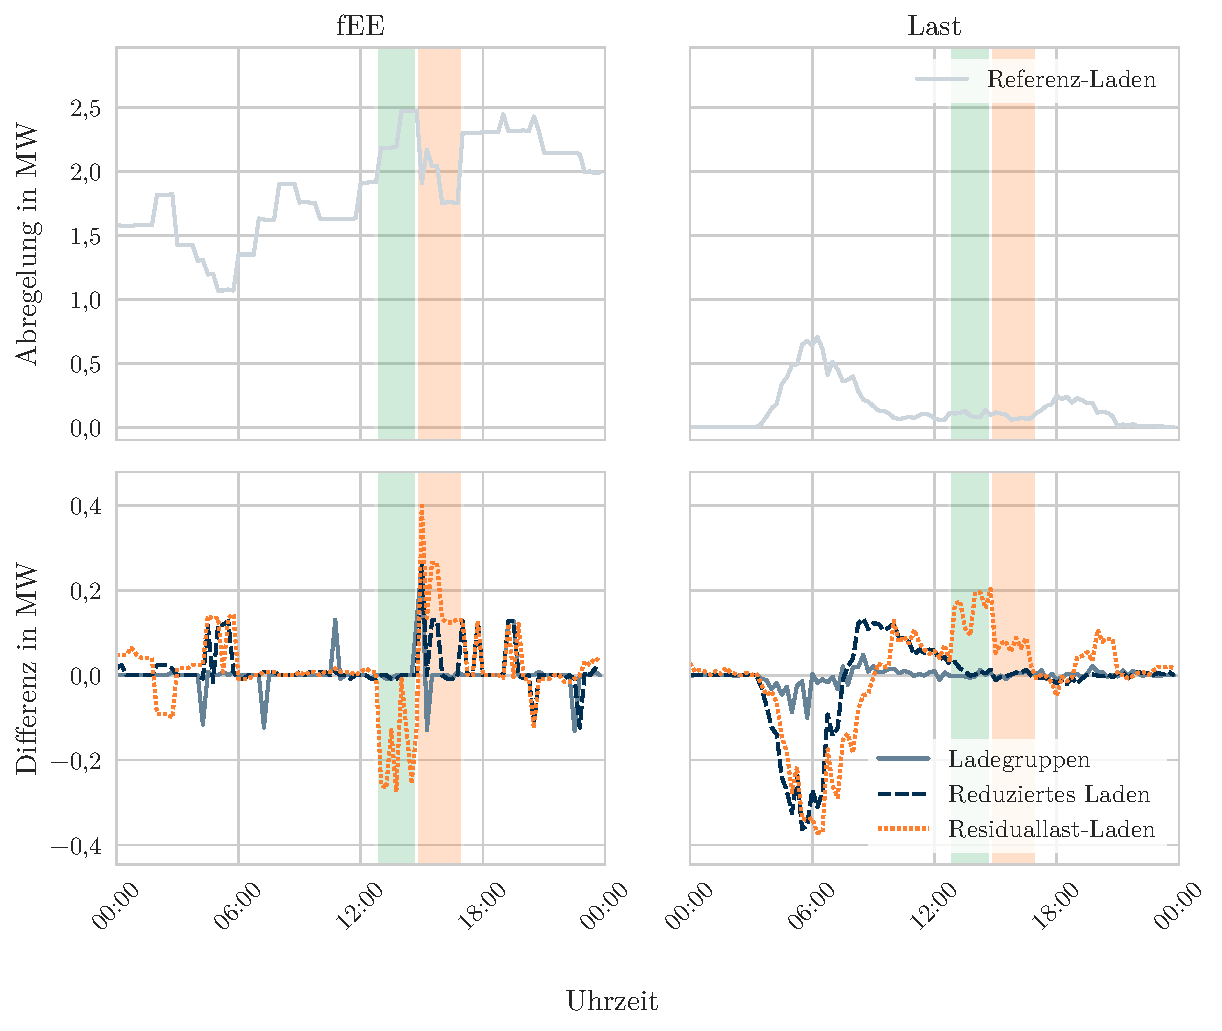
\includegraphics[width=\textwidth]{Bilder/1690_fEE_load_diff}
    \caption{Durchschnittliche Abregelung von fEE Anlagen (oben links) und Lasten (oben rechts) innerhalb von Woche~MIN und die durchschnittliche Differenz des Abregelungsbedarfs der Ladestrategien gegenüber dem Referenz-Laden für fEE Anlagen (unten links) und Lasten (unten rechts) im Antriebswende-Szenario im Netz \num{1690}}\label{fig:1690_fEE_load_diff}
\end{figure}

Im roten Bereich kommt es ebenfalls zu einem erhöhten Ladebedarf des \UC \Firmeparkplatzdot.
Diese Erhöhung fällt jedoch geringer aus als im grünen Bereich und der lastseitige Abregelungsbedarf wird entsprechend weniger stark erhöht.
Gleichzeitig wird der Ladebedarf des \UCs \zH gegenüber der Referenz-Ladestrategie abgesenkt, da die Residuallast in der Regel nachts niedriger ausfällt als in diesem Zeitfenster und die Ladevorgänge \zH somit vermehrt nachts stattfinden.
Innerhalb der \gls{NS}-Netze in denen primär Ladevorgänge \zH stattfinden, befinden sich im \gls{MS}-Netz \(1690_{\text{W}}\) viele \glspl{PVA}.
Hierdurch erhöht sich sowohl der erzeugerseitige \gls{NS}- als auch \gls{MS}-Abregelungsbedarf.
Windkraftanlagen befinden sich demgegenüber nicht in der örtlichen Nähe der \gls{NS}-Netze in denen primär Ladevorgänge \zH stattfinden.
Da es jedoch nachts ausschließlich zu Abregelungen von Windkraftanlagen kommt, wird der nächtliche Abregelungsbedarf durch die Ladevorgänge nur wenig beeinflusst.


\paragraph{Fazit:}

In den Wind-dominierten Netzen kommt es lastseitig vor allem zu Abregelungen auf der \gls{NS}-Ebene, da die \gls{MS}-Ebene in der Regel gut ausgebaut ist.
Erzeugerseitige Abregelung findet nur im Netz \(1690_{\text{W}}\) statt.\medskip

Auch bei den Wind-domninierten Netzen zeigen sich die Ladegruppen als weitgehend ineffektiv und kann den lastseitigen Abregelungsbedarf nur leicht reduzieren.
Das reduzierte Laden kann hingegen in der Regel einen großen Anteil des lastseitigen Abregelungsbedarfs verhindern, wobei sich bestätigt, dass das Einsparpotential mit einer zunehmenden Belastung der \gls{NS}-Netze abnimmt.
Das aktive Residuallast-Laden erweist sich lastseitig in den Wind-dominierten Netzen als weniger effektiv als das reduzierte Laden.
Aufgrund des hohen Verhältnisses zwischen Einspeisung und Ladebedarf kommt es beim Residuallast-Laden zu einer hohen Konzentration des Ladebedarfs auf wenige Zeitschritte.
Hierdurch kann der lastseitige Abregelungsbedarf, trotz einer starken Reduktion am Morgen, insgesamt nur leicht gesenkt werden, da der Abregelungsbedarf am Nachmittag stark zunimmt.\medskip

Der Abregelungsbedarf von \gls{FEE} Anlagen kann durch die untersuchten Ladestrategien zum einen nur in einem sehr geringen Maße und zum anderen nicht positiv beeinflusst werden.
So richtet sich das Residuallast-Laden nach einer globalen Residuallast im \gls{MS}-Netz die keine lokalen Unterschiede beachtet.
So werden Ladevorgänge zwar zeitlich in günstige Zeitfenster verschoben, aber diese finden an ungünstigen Lokalitäten statt, wodurch sich der Abregelungsbedarf sogar weiter erhöht.
Es empfiehlt sich somit, die lokale Netztopologie mit in die Priorisierung der Ladevorgänge einzubeziehen, um eine ungünstige lokale Verteilung der Ladevorgänge zu vermeiden.


\subsubsection{Last-dominiertes Netz}

In dem Last-dominierten Netz \(177_{\text{L}}\) kommt es in Woche~MIN im Antriebswende-Szenario zu einem annähernd ausgewogenen Verhältnis zwischen der Einspeisung aus \gls{FEE} Anlagen und dem Ladebedarf der \gls{EPKW}.
In Woche~MAX kommt es hingegen nur zu einer minimalen Einspeisung aus \gls{FEE} Anlagen.
Die wichtigsten Eckdaten des Netzes \(177_{\text{L}}\) finden sich in \autoref{tab:load_dominated_char} und der Ladebedarf je Szenario findet sich in \autoref{tab:load_dominated_epkw_demand}.

{
\renewcommand{\arraystretch}{1.2}% grßerer Zeilenabstand
\sisetup{range-phrase=~{--}~}% Gedankenstrich statt "bis" bei SIrange
\begin{table}[H]
	\begin{center}
		\caption{Einspeisung von fEE und nicht-fEE Anlagen sowie der Bedarf von sonstigen Lasten in dem Last-dominierten Netz}
		\begin{tabu} to 0.7\textwidth {X[2] X[1, r] X[1, r]}
			\toprule
											  & Woche A      & Woche B      \\ \midrule
			Einspeisung fEE in \si{\mwh}      & \num{871.5}  & \num{51.8}   \\
			Einspeisung Sonstige in \si{\mwh} & \num{47.2}   & \num{47.2}   \\
			Bedarf Sonstige  in \si{\mwh}     & \num{5413.0} & \num{5716.0} \\ \bottomrule
		\end{tabu}
		\label{tab:load_dominated_char}
	\end{center}
	\vspace{-3mm}%Put here to reduce too much white space after your table
\end{table}
}

{
\renewcommand{\arraystretch}{1.2}% grßerer Zeilenabstand
\sisetup{range-phrase=~{--}~}% Gedankenstrich statt "bis" bei SIrange
\begin{table}[H]
	\begin{center}
		\caption{Ladebedarf der E-Pkw im Last-dominierten Netz je Szenario}
		\begin{tabu} to 0.6\textwidth {X[1.5] X[1, r] X[1, r]}
			\toprule
			Ladebedarf\(^*\) in   \si{\mwh}    & Woche~MIN     & Woche~MAX     \\ \midrule
			NEP C~\num{2035}             & \num{271.3} & \num{271.3} \\
			Referenz                     & \num{485.3} & \num{485.3} \\
			Antriebswende                & \num{919.0} & \num{919.0} \\
			\glqq Firmenparkplatz\grqq{} & \num{915.3} & \num{915.3} \\ \bottomrule
			\multicolumn{3}{l}{\(^*\)netzseitiger Ladebedarf (inkl. Umwandlungsverluste)}
		\end{tabu}
		\label{tab:load_dominated_epkw_demand}
	\end{center}
	\vspace{-3mm}%Put here to reduce too much white space after your table
\end{table}
}

Bei dem Abregelunsgbedarf des Ladebedarfs der \gls{EPKW} beim Referenz-Laden nach \autoref{tab:load_dominated_epkw_cur} zeigt sich ein ähnliches Verhalten wie in dem \gls{PV}-dominierten Netz \(176_{\text{PV}}\), da es auch im Netz \(177_{\text{L}}\) nach \autoref{tab:largestLVGridShare} zu einer starken Konzentration des Ladebedarfs in wenigen \gls{NS}-Netzen kommt.
So muss in jedem Szenario ein großer Anteil des Ladebedarfs abgeregelt werden, weil einzelne \gls{NS}-Netze stark überlastet werden.
Im Antriebswende-Szenario entfallen in Woche~MIN \SI{98}{\percent} des Abregelungsbedarf auf die \gls{NS}-Ebene, wobei bereits drei \gls{NS}-Netze mehr als \SI{60}{\percent} des Abregelungsbedarfs ausmachen.
Im Gegensatz zum Netz \(176_{\text{PV}}\) kommt es nach \autoref{tab:load_dominated_load_cur} in dem Last-dominierten Netz zusätzlich zu einem größeren Anteil an Abregelung von sonstigen Lasten.

{
\renewcommand{\arraystretch}{1.2}% grßerer Zeilenabstand
\sisetup{range-phrase=~{--}~}% Gedankenstrich statt "bis" bei SIrange
\begin{table}[H]
	\begin{center}
		\caption{Abregelungsbedarf des Ladebedarfs von E-Pkw in dem Last-dominierten Netz je Szenario für die Referenz-Ladestrategie}
		\begin{tabu} to 0.6\textwidth {X[1.5] X[1, r] X[1, r]}
			\toprule
			Abregelung in   \si{\mwh}    & Woche~MIN     & Woche~MAX     \\ \midrule
			NEP C~\num{2035}             & \num{60.5}  & \num{68.9}  \\
			Referenz                     & \num{147.4} & \num{160.8} \\
			Antriebswende                & \num{337.8} & \num{360.9} \\
			\glqq Firmenparkplatz\grqq{} & \num{381.5} & \num{405.5} \\ \bottomrule
		\end{tabu}
		\label{tab:load_dominated_epkw_cur}
	\end{center}
	\vspace{-3mm}%Put here to reduce too much white space after your table
\end{table}
}

{
\renewcommand{\arraystretch}{1.2}% grßerer Zeilenabstand
\sisetup{range-phrase=~{--}~}% Gedankenstrich statt "bis" bei SIrange
\begin{table}[H]
	\begin{center}
		\caption{Abregelungsbedarf der sonstigen Lasten im Last-dominierten Netz je Szenario für die Referenz-Ladestrategie}
		\begin{tabu} to 0.6\textwidth {X[1.5] X[1, r] X[1, r]}
			\toprule
			Abregelung in   \si{\mwh}    & Woche A     & Woche B     \\ \midrule
			NEP C~\num{2035}             & \num{179.6} & \num{247.7} \\
			Referenz                     & \num{211.7} & \num{274.3} \\
			Antriebswende                & \num{253.1} & \num{318.5} \\
			\glqq Firmenparkplatz\grqq{} & \num{253.2} & \num{319.5} \\ \bottomrule
		\end{tabu}
		\label{tab:load_dominated_load_cur}
	\end{center}
	\vspace{-3mm}%Put here to reduce too much white space after your table
\end{table}
}

In \autoref{fig:177_cur_load_both_weeks} findet sich die Veränderung des lastseitigen Abregelungsbedarfs aufgrund der Ladestrategien gegenüber dem Referenz-Laden für die beiden untersuchten Wochen.
Auch bei dem Last-dominierten Netz erweist sich das reduzierte Laden am effektivsten, um den lastseitigen Abregelungsbedarf zu senken.
Dabei fällt das relative Senkungspotential des Abregelungsbedarfs aufgrund der hohen Auslastung der \gls{NS}-Netze in allen Szenarien verhältnismäßig niedrig aus.
Durch das Residuallast-Laden kann die Abregelung in der Regel in einem ähnlichen Maße gesenkt werden, wie durch das reduzierte Laden.
Demgegenüber kann durch die Ladegruppen der Abregelungsbedarf nur leicht gesenkt werden und erweist sich somit auch in dem Last-dominierten Netz als wenig effektiv.

\begin{figure}[H]
    \centering
    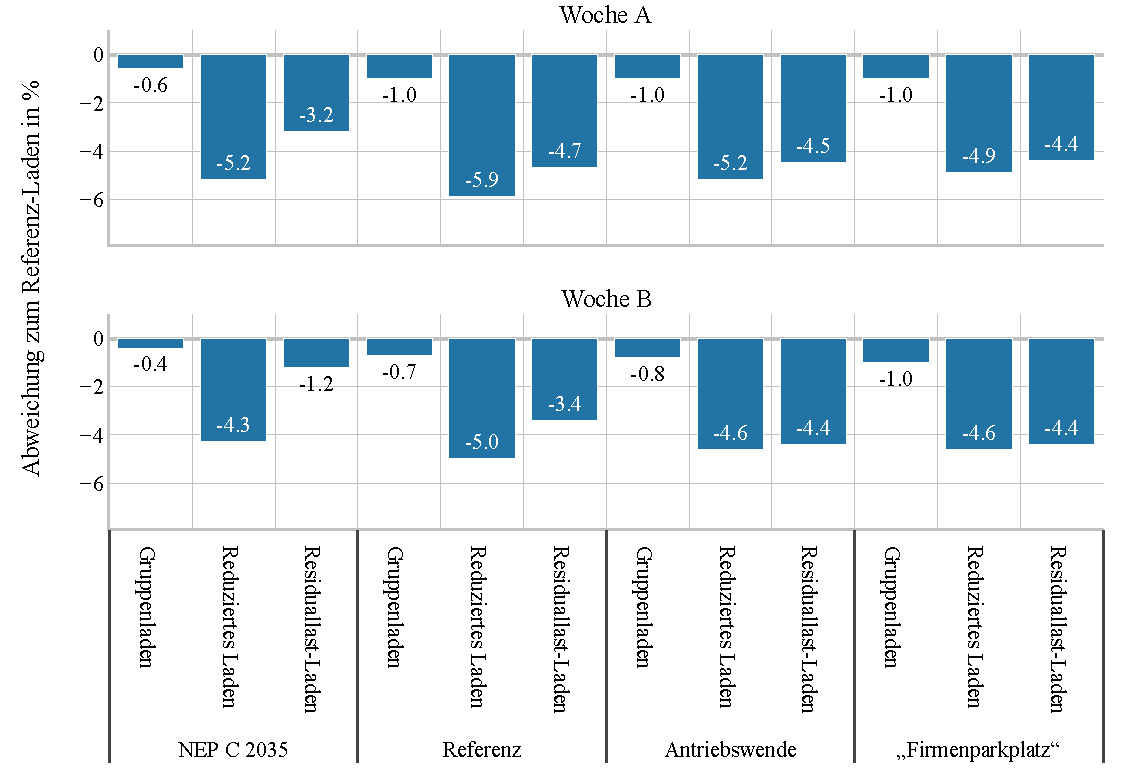
\includegraphics[width=\textwidth]{Bilder/177_cur_load_both_weeks}
    \caption{Prozentuale Veränderung des Abregelungsbedarfs von allen Lasten in Abhängigkeit von der Ladestrategie in Woche~A (oben) und Woche~B (unten) gegenüber dem Abregelungsbedarf für die Referenz-Ladestrategie je Szenario für das Netz \num{177}}\label{fig:177_cur_load_both_weeks}
\end{figure}

In \autoref{fig:177_load_diff} findet sich die durchschnittliche Abregelung von Lasten im Antriebswende-Szenario innerhalb von Woche~MIN beim Referenz-Laden (oben) und die Differenz des Abregelungsbedarfs zwischen den Ladestrategien und dem Referenz-Laden (unten).
Demnach kommt es im Durchschnitt im Netz \(177_{\text{L}}\) in den meisten Zeitschritten zu einem starken Abregelungsbedarf.
Hiervon ausgenommen ist in allen Szenarien die Nacht in der es nur selten zu lastseitiger Abregelung kommt.\medskip

Beim reduzierten Laden kann am Morgen und ab dem Mittag bis zum Abend lastseitige Abregelung verhindert werden.
Demgegenüber erhöht sich der Abregelungsbedarf in den verbleibenden Zeitschritten.
Der Ladebedarf des \UC \Firmeparkplatz wird vom morgen in den Vormittag gestreckt, wodurch der Ladebedarf in Zeiten verschoben wird, in denen auch die Einspeisung der \glspl{PVA} höher ausfällt.
Zusätzlich wird Ladebedarf \zH in die nächtliche Schwachlastzeit verschoben.
Durch diese zwei günstigen zeitlichen Verschiebungen des Ladebedarfs kommt es insgesamt zu einer Reduktion des lastseitigen Abregelungsbedarfs.

\begin{figure}[H]
    \centering
    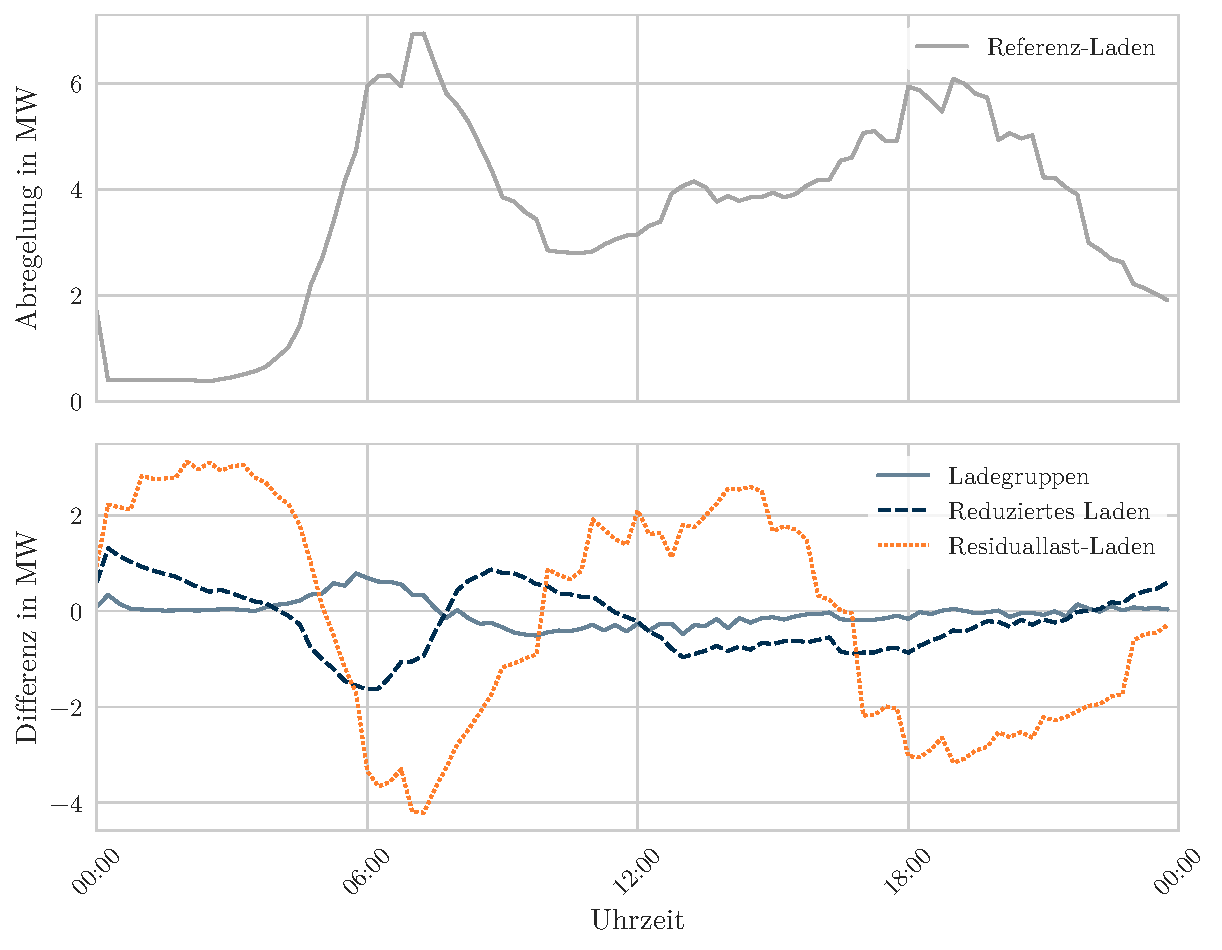
\includegraphics[width=\textwidth]{Bilder/177_load_diff}
    \caption{Durchschnittliche Abregelung von Lasten (oben) innerhalb von Woche~MIN und die durchschnittliche Differenz des Abregelungsbedarfs der Ladestrategien gegenüber dem Referenz-Laden für Lasten (unten) im Antriebswende-Szenario im Netz \num{177}}\label{fig:177_load_diff}
\end{figure}

Beim Residuallast-Laden zeigt sich ein ähnlicher Trend wie beim reduzierten Laden, wobei die Verschiebung der Last wesentlich stärker ausgeprägt ist.
Der Abregelungsbedarf erhöht sich nachts deutlich, während die Abregelung am Abend stark abgesenkt werden kann.
Am Morgen und am Vormittag kann durch die Verschiebung des Ladebedarfs in die Hochzeit der Einspeisung ein großer Anteil an Abregelung verhindert werden.
Da einige \gls{NS}-Netze in der Mittagszeit bereits beim Referenz-Laden überlastet sind, erhöht sich der lastseitige Abregelungsbedarf im Schnitt deutlich.
Insgesamt kann auf diese Weise nur eine moderate Reduktion des lastseitigen Abregelungsbedarfs erreicht werden.\medskip

Im Netz \(177_{\text{L}}\) kommt es im Gegensatz zu den zuvor untersuchten Netzen zu einer verstärkten lastseitigen Abregelung auf der \gls{MS}-Ebene.
Diese ist aufgrund der geringen installierten Leistung von \gls{FEE} Anlagen weniger stark ausgebaut als in den zuvor betrachteten Netzen.
Da nach \autoref{tab:largestLVGridShare} im Netz \(177_{\text{L}}\) zusätzlich ein besonders hoher Anteil von Ladestationen direkt in der \gls{MS}-Ebene angeschlossen ist, kommt es beim Referenz-Laden bereits zu einem hohen Anteil von reduzierten Ladevorgängen.
Hiervon sind vor allem Ladestationen des \UCs \Firmeparkplatz betroffen.
Da gegenüber den reduzierten Ladevorgängen bei den Ladegruppen der Ladebedarf zeitlich weniger gestreckt wird, kommt es am morgen kurzzeitig zu einem erhöhten Abregelungsbedarf, welcher in \autoref{fig:177_load_diff} nachvollzogen werden kann.

{
\renewcommand{\arraystretch}{1.2}% grßerer Zeilenabstand
\sisetup{range-phrase=~{--}~}% Gedankenstrich statt "bis" bei SIrange
\begin{table}[H]
	\begin{center}
		\caption{Abregelungsbedarf von fEE im Last-domnierten Netz je Szenario für die Referenz-Ladestrategie}
		\begin{tabu} to 0.6\textwidth {X[1.5] X[1, r] X[1, r]}
			\toprule
			Abregelung in   \si{\mwh}    & Woche~MIN   & Woche~MAX   \\ \midrule
			NEP C~\num{2035}             & \num{0.7} & \num{0.0} \\
			Referenz                     & \num{0.5} & \num{0.0} \\
			Antriebswende                & \num{0.3} & \num{0.0} \\
			\glqq Firmenparkplatz\grqq{} & \num{0.2} & \num{0.0} \\ \bottomrule
		\end{tabu}
		\label{tab:load_dominated_fee_cur}
	\end{center}
	\vspace{-3mm}%Put here to reduce too much white space after your table
\end{table}
}

Der Abregelungsbedarf von \gls{FEE} Anlagen fällt im Netz \(177_{\text{L}}\) nach \autoref{tab:load_dominated_fee_cur} mit maximal \SI{0.7}{\mwh} sehr gering aus und macht in Woche~MIN weniger als \SI{0.1}{\percent} der Einspeisung von \gls{FEE} Anlagen aus.
Auch beschränkt sich der Abregelungsbedarf auf einige wenige Zeitschritte am frühen Nachmittag in einem einzigen \gls{NS}-Netz.
Dementsprechend führen nach \autoref{fig:177_cur_fee_grid_week_A} bereits kleine absolute Änderungen im Abregelungsbedarf zu großen relativen Ausschlägen.
So erhöht sich der erzeugerseitige Abregelungsbedarf in dem Last-dominierten Netz wie bei den \gls{PV}-dominierten Netzen sowohl durch die Ladegruppen als auch das reduzierte Laden.
Da es ausschließlich in einem \gls{NS}-Netz mit einem hohen Anteil an Ladevorgängen \zH zu einer Abregelung von \gls{FEE} Anlagen kommt, kommt es durch die Reduktion des Ladebedarfs am frühen Nachmittag beim Gruppen- und reduzierten Laden (vgl. \autoref{fig:residual_load_diff}) zu einer stärkeren Erhöhung des Abregelungsbedarfs in der \SzeFirmenparkplatz im Vergleich zu den anderen Szenarien.

\begin{figure}[H]
    \centering
    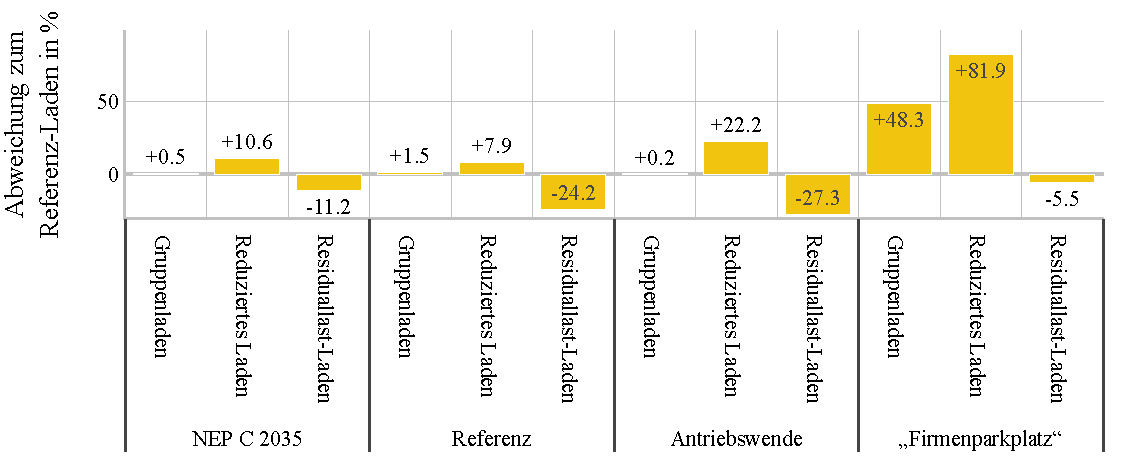
\includegraphics[width=\textwidth]{Bilder/177_cur_fee_grid_week_A}
    \caption[Prozentuale Veränderung des Abregelungsbedarfs von fEE Anlagen in Abhängigkeit von der Ladestrategie in Woche~MIN gegenüber dem Abregelungsbedarf für die Referenz-Ladestrategie je Szenario für das Netze \num{177}]{Prozentuale Veränderung des Abregelungsbedarfs von fEE Anlagen in Abhängigkeit von der Ladestrategie in Woche~MIN gegenüber dem Abregelungsbedarf für die Referenz-Ladestrategie je Szenario für das Netze \(177_{\text{L}}\)}\label{fig:177_cur_fee_grid_week_A}
\end{figure}

Grundsätzlich kann durch die Residuallast-Ladestrategie der Abregelungsbedarf der \gls{FEE} Anlagen gesenkt werden.
Da innerhalb des von erzeugerseitiger Abregelung betroffenen \gls{NS}-Netzes jedoch ein signifikanter Anteil des Ladebedarfs in die Nacht verschoben wird und sich der Ladebedarf am frühen Nachmittag gegenüber der Referenz-Ladestrategie nur gering verändert, kann der Abregelungsbedarf in absoluten Zahlen nur wenig gesenkt werden.
Da dies vor allem für Ladevorgänge \zH gilt, verstärkt sich dieser Effekt in der \SzeFirmenparkplatzdot, weshalb das Einsparpotential hierbei geringer ausfällt.


\paragraph{Fazit:}

Insgesamt zeigt das Last-dominierte Netz \(177_{\text{L}}\) aufgrund der hohen Konzentration des Ladebedarfs in einigen wenigen \gls{NS}-Netzen viele Parallelen zu dem \gls{PV}-dominierten Netz \(176_{\text{PV}}\).
Durch den geringeren \gls{PV}-Anteil im Netz \(177_{\text{L}}\) ist das Netz insgesamt jedoch weniger stark ausgebaut, weshalb es zu einem deutlich höheren lastseitigen Abregelungsbedarf kommt, während der erzeugerseitige Abregelungsbedarf minimal ausfällt.\medskip

In dem Last-dominierten Netz bestätigt sich wiederholt die geringe Effektivität der Ladegruppen.
Das reduzierte Laden kann hingegen den lastseitigen Abregelungsbedarf am effektivsten senken, da der Ladebedarf teilweise noch erfolgreich in die nächtliche Schwachlastzeit und in das Einspeisezeitfenster der \glspl{PVA} im Verlaufe des Tages verschoben werden kann.
Das Residuallast-Laden weist einen ähnlichen Verlauf auf.
Jedoch kommt es hierbei zu einer starken Übersteuerung, weshalb der Abregelungsbedarf nur in einem geringeren Maße als beim reduzierten Laden gesenkt werden kann.
Insgesamt fällt das Potential lastseitige Abregelung zu verhindern aufgrund der hohen Überlastung einzelner \gls{NS}-Netze gering aus.\medskip

Der Abregelungsbedarf von \gls{FEE} Anlagen erhöht sich durch die präventiven Ladestrategien, da der Ladebedarf in den Hochzeiten der Einspeisung am frühen Nachmittag reduziert wird.
Das Residuallast-Laden kann hingegen den erzeugerseitigen Abregelungsbedarf senken.
Da jedoch ein signifikanter Anteil des Ladebedarfs \zH in die Nacht verschoben wird, fällt das Einsparpotential verhältnismäßig gering aus.

\clearpage


\section{Schlussbetrachtung und Ausblick}\label{chap:schlussbetrachtung}

Das Ziel dieser Arbeit war es, die Auswirkungen verschiedener präventiver und aktiver Ladestrategien bei unterschiedlichen Durchdringungstiefen von \glspl{EPKW} auf die drei Netzgebietsklassen \gls{PV}-, Wind- und Last-dominiert aufzuzeigen.
Dafür wurde der jeweils nötige last- und erzeugerseitige Abregelungsbedarf innerhalb der untersuchten \gls{MS}-Netze inklusive darunterliegender \gls{NS}-Netze quantifiziert.\medskip

Mit \glsi{SIMBEV} wurde ein Software Tool mitentwicklet, mit dessen Hilfe plausible Fahrtprofile von \gls{EPKW} erzeugt werden können.
Die Fahrtprofile zeigen, dass ein Großteil der Ladevorgänge im privaten Bereich stattfindet.
Bei privaten Ladevorgängen wird zudem ersichtlich, dass die Ladung der \glspl{EPKW} nur einen geringen Anteil der Standzeit ausmacht.
In den untersuchten Szenarien entstehen die stärksten Leistungsspitzen am Morgen durch das Laden am Arbeitsplatz, während das Laden zu Hause den größten Energiebedarf aufweist.
Die anschließende Verortung des Ladebedarfs führt teilweise zu unplausiblen Belastungen einzelner \gls{NS}-Netze innerhalb der Referenznetzgebiete.
In der Realität würde in solchen Situationen vermutlich ein umfänglicher Netzausbau oder sogar ein Netzneubau vorgenommen, welches innerhalb dieser Arbeit nicht abgebildet werden kann.\medskip

Mit einem steigenden Ladebedarf, aufgrund eines erhöhten Hochlaufs der \glspl{EPKW} in den Szenarien nimmt der Bedarf an lastseitigen Abregelungen in den meisten Referenznetzgebieten immer stärker zu.
Hierdurch verringert sich das relative Senkungspotential des lastseitigen Abregelungsbedarfs, da der Abregelungsbedarf verstärkt verschoben, jedoch nicht verhindert werden kann.
Die Untersuchung der \SzeFirmenparkplatz ergibt, dass beim Referenz-Laden in den meisten Fällen der Bedarf an last- und erzeugerseitiger Abregelung im Vergleich zum Antriebswende-Szenario geringer ausfällt.
Hierfür verantwortlich ist in der Regel der hohe Anteil an \glspl{PVA} in den \gls{NS}-Netzen mit einem hohen Anteil an Ladevorgängen des \UC \zHdot.
Sind diese \gls{NS}-Netze lastseitig bereits stark ausgelastet, dann erhöht sich der lastseitige Abregelungsbedarf in der \SzeFirmenparkplatz gegenüber dem Antriebswende-Szenario.\medskip

Bei den Ladestrategien führen die präventiven Ladestrategien zu einer Erhöhung der Spreizung zwischen der maximalen und minimalen Residuallast.
Dies kann als Indikator für eine möglicherweise benötigte Erhöhung der Dimensionierung der Netze gegenüber dem Referenz-Laden gedeutet werden.
Der negative Effekt der präventiven Ladestrategien lässt sich primär in Netzen mit einem hohen Anteil an \glspl{PVA} beobachten.
Am frühen Nachmittag ist in diesen Netzen aufgrund der präventiven Ladestrategien ein geringerer Ladebedarf zu verzeichnen.
Da in diesem Zeitfenster die Einspeisung der \glspl{PVA} in der Regel hoch ausfällt, wird die Residuallast gesenkt.
Von diesem Effekt sind in erster Linie Ladevorgänge des \UC \zH betroffen.
Da in \gls{NS}-Netzen mit einem hohen Anteil an Ladevorgängen des \UC \zH in der Regel auch viele \glspl{PVA} verortet sind, erhöht sich in diesen Fällen aufgrund der präventiven Ladestrategien der Abregelungsbedarf von \gls{FEE}.
Dies gilt vor allem für die \gls{PV}-dominierten Netze.
Aufgrund der in den Netzen installierten \gls{PV}-Kapazitäten sind jedoch auch die Wind- und Last-dominierten Netze hiervon betroffen.
In den Wind-dominierten Netzen fällt der Effekt aufgrund des niedrigeren Anteils von \glspl{PVA} an den Erzeugerkapazitäten relativ geringer aus.\medskip

Im Gegensatz zu den präventiven Ladestrategien kann durch das Residuallast-Laden sowohl der maximale Last- als auch Einspeisefall im Netzgebiet gesenkt werden.
Erweiternd kann der Abregelungsbedarf von \gls{FEE} in den \gls{PV}- und Last-dominierten Netzen gesenkt werden.
Hierbei werden viele Ladevorgänge in die Mittagszeit verschoben und es findet ein besserer Ausgleich zwischen Last und Erzeugung statt.
In den Wind-dominierten Netzen zeigt sich demgegenüber ein erhöhter Abregelungsbedarf von \gls{FEE}, wobei sich zwei Effekte beobachten lassen.
Zum einen befindet sich in den Wind-dominierten Netzen zusätzlich ein gewisser Anteil an \glspl{PVA}, welcher wie zuvor beschrieben vermehrt in \gls{NS}-Netzen mit einem hohen Anteil an Ladevorgängen des \UC \zH verortet ist.
Aufgrund einer niedrigen Residuallast in der Nacht werden viele Ladevorgänge des \UC \zH in die Nacht verschoben.
Zum anderen befinden sich Wind-Kapazitäten nicht in örtlicher Nähe zu der privaten Ladeinfrastruktur und werden auf der \gls{MS}-Ebene angeschlossen.
Hierdurch wird der Abregelungsbedarf der Wind-Kapazitäten durch die Ladestrategien kaum beeinflusst, während sich der Abregelungsbedarf der \glspl{PVA}, und somit in Summe der Abregelungsbedarf von \gls{FEE}, erhöht.\medskip

Der lastseitige Abregelungsbedarf kann in den meisten Fällen sowohl durch das reduzierte Laden als auch das Residuallast-Laden gesenkt werden.
Dabei ist insbesondere der Erfolg des Residuallast-Ladens von mehreren Randbedingungen abhängig.
Zum einen ist es aufgrund von Ausgleichseffekten zwischen der Last und Erzeugung entscheidend, ob sich die Erzeugerkapazitäten in den gleichen \gls{NS}-Netzen befinden, in denen auch die Ladevorgänge stattfinden, und ob Ladevorgänge und Einspeisung innerhalb eines \gls{NS}-Netzes gleichzeitig stattfinden.
Zum anderen ist von großer Bedeutung, wie stark die einzelnen \gls{NS}-Netze ausgelastet sind.
Wenn ein \gls{NS}-Netz bereits innerhalb des Großteils der Zeitpunkte überlastet ist, kann der lastseitige Abregelungsbedarf in der Regel nur noch verschoben, jedoch nicht verhindert werden.
Sind diese Bedingungen gegeben, kann durch das Residuallast-Laden ein hoher Anteil des lastseitigen Abregelungsbedarfs vermieden werden.
Ist dies hingegen nicht der Fall, führen hohe Gleichzeitigkeiten, welche durch das Residuallast-Laden entstehen können, zu negativen lastseitigen Auswirkungen.
So entsteht primär in den Wind-dominierten Netzen der Effekt, dass sich das Residuallast-Laden an einer globalen Residuallast im gesamten Netzgebiet orientiert, welche nur bedingt die lokale Situation in den einzelnen \gls{NS}-Netzen widerspiegelt.
In diesen Fällen erweist sich das reduzierte Laden als besser geeignet, um den lastseitigen Abregelungsbedarf zu senken.
Die Ladegruppen führen hingegen nur zu einer geringen Senkung dieses gegenüber dem Referenz-Laden.
So kann die Gleichzeitigkeit durch die Ladegruppen nur in einem geringen Maße beeinflusst werden.
Auf der \gls{MS}-Ebene erhöht sich zudem die maximale Last gegenüber dem Referenz-Laden, da reduzierte Ladevorgänge durch Ladevorgänge in Ladegruppen ersetzt werden.\medskip

Zusammenfassend zeigt sich, dass sowohl präventive als auch aktive Ladestrategien die Netzintegration von \gls{EPKW} unterstützen können.
Das präventive reduzierte Laden erweist sich als besonders erfolgreich den lastseitigen Abregelungsbedarf zu mindern.
Demgegenüber können durch die ebenfalls präventiven Ladegruppen keine signifikanten Reduzierungen des Abregelungsbedarfs erreicht werden.
Unter den richtigen Bedingungen kann der lastseitige Abregelungsbedarf durch das aktive Residuallast-Laden am stärksten gesenkt werden.
Erweiternd kann das Residuallast-Laden auch die Netzintegration von \gls{FEE} unterstützen.
Dies können die präventiven Ladestrategien nicht leisten und führen sogar zu einer Verschlechterung des Abregelungsbedarfs von \gls{FEE}.
Der Erfolg des Residuallast-Ladens ist davon abhängig, ob die globale Residuallast im \gls{MS}-Netzgebiet die Situationen in den einzelnen \gls{NS}-Netzen näherungsweise gut widerspiegelt.
Ist dies nicht gegeben, erweist sich das reduzierte Laden als die beste Alternative, um den lastseitigen Abregelungsbedarf zu minimieren und somit die Netzintegration von \glspl{EPKW} zu unterstützen.\medskip

Neben den untersuchten Ladestrategien, gibt es noch eine Vielzahl von denkbaren Ladestrategien, welche ebenfalls auf ihre netzdienlichen Effekte untersucht werden sollten.
Erweiternd zu den netzdienlichen Ladestrategien sollte auch bei der Verortung der Ladeinfrastruktur auf ein möglichst netzdienliches Vorgehen geachtet werden, indem Gegebenheiten des Netzes miteinbezogen werden.
Weiterhin sollte \glsi{SIMBEV} dahingehend erweitert werden, einen Zeitraum von mindestens einem Jahr und saisonale Schwankungen im Verbrauch der \gls{EPKW} und dem Fahrtverhalten der Fahrzeugnutzer\(^*\)innen abbilden zu können.
Hierdurch würde die Realitätsnähe des Tools erhöht und eine größere Anzahl von unterschiedlichen Bedarfsfällen abgedeckt werden.\medskip

Konkret sollte geprüft werden, ob das Residuallast-Laden erweitert und dadurch verbessert werden kann.
Hierbei sollten zwei Optionen untersucht werden, wobei darauf zu achten ist, dass diese Konzepte auch in der Realität abgebildet werden können.
Zum einen können dem Residuallast-Laden Randbedingungen hinzugefügt werden.
So kann beispielsweise die Belastungsgrenze der jeweiligen \gls{ONS} beachtet werden und/oder die Wirkleistung der installierten \gls{FEE} Erzeugerkapazitäten in den \gls{NS}-Netzen als ein Gewichtungsfaktor in die Ladestrategie mit eingehen.
Zum anderen kann statt der globalen Residuallast innerhalb des Netzgebietes auch die Residuallast einzelner Abschnitte des Netzgebietes als Leitlinie dienen.
Hierbei kann beispielsweise die Residuallast der einzelnen \gls{MS}-Abgänge oder sogar die Residuallast einzelner \gls{NS}-Netze genutzt werden.
Es ist zu vermuten, dass aufgrund dieser Maßnahmen lokale Engpässe in den Netzen besser berücksichtigt werden und die Netzintegration von \gls{EPKW} stärker unterstützt werden kann.

% je mehr MS Ebene, desto besser wird Referenz-Laden ggü den Ladegruppen

%\newpage

%\section{Einleitung}

\lipsum[24]

% You need inkscape for this
% inkscape needs to be in your PATH
\begin{figure}[H]
    \centering
    \includesvg[width=\textwidth]{Bilder/SurfPlot}
    \caption{Beispiel eines \texttt{Surface Plots} der drei Gleichungen des Gleichungssystems $A\vec{x} = \vec{b}$ nach $x_3$ aufgelöst}\label{fig:SurfPlot}
\end{figure}

In \autoref{fig:SurfPlot} findet sich ein Beispiel für eine \texttt{SVG}-Grafik. \lipsum[13]

\section{Theoretische Grundlagen}

\lipsum[32]

\begin{equation}
	E = \hbar \omega
	\label{eq:plancksrelation}
\end{equation}

\autoref{eq:plancksrelation} zeigt ein Beispiel für eine Gleichung. \lipsum

\section{Methodik}

\lipsum[27]

%{
\renewcommand{\arraystretch}{1.2}% grßerer Zeilenabstand
\sisetup{range-phrase=~{--}~}% Gedankenstrich statt "bis" bei SIrange
\begin{table}[H]
	\begin{center}
		\caption{Emissionsfaktoren von Biogasanlagen mit direkter Biogasverbrennung}
		\begin{tabu} to \textwidth {X X[1.5, r]}
			\hline
			Schadstoff	& Emissionen in \si[per-mode=symbol]{\mgkwh}					\\ \hline
			\ce{CO}		& \SIrange{922}{1116}{\relax}                               	\\
			\ce{SO2}	& \SI{90}{\relax}                                       		\\
			\ce{NO_X}	& \SIrange{727}{1944}{\relax}                               	\\
			\ce{NMVOC}	& \SIrange{36}{76}{\relax}                                  	\\
			\ce{CH2O}	& \SIrange{31}{50}{\relax}                                  	\\ \hline
			\multicolumn{2}{l}{Quellen: \cite{Paolini2018}}
		\end{tabu}
		\label{tab:tab_air-pollutants}
	\end{center}
	\vspace{-3mm}%Put here to reduce too much white space after your table
\end{table}
}

\autoref{tab:tab_air-pollutants} zeigt ein Beispiel für eine Tabelle. \lipsum

\section{Ergebnisse}

\lipsum[14]

\begin{code}
    \captionof{listing}{Gaußsches Eliminationsverfahren}\label{code:GaussElem}
    \begin{minted}[
		linenos=true,
		numbersep=-10pt,
		obeytabs=true,
		tabsize=4,
		]{matlab}
		%% Gaussian Elimination
		% bringing the Matrix into upper triangular form
		% initializing a new matrix to keep the previous results
		GaussMat = OrdMat;
		% and a new vector
		GaussVec = OrdVec;
		% for loop over m-1 elements
		for i = 1:m-1
		   % Calculating the Row Multiplier by dividing the
		   % i Element of the row i+1:m through the
		   % i,i Element of the matrix
		   Mult = GaussMat(i+1:m,i) / GaussMat(i,i);
		   % Calculating the new rows of the matrix
		   GaussMat(i+1:m,:) = GaussMat(i+1:m,:) - Mult*GaussMat(i,:);
		   % and the vector
		   GaussVec(i+1:m,:) = GaussVec(i+1:m,:) - Mult*GaussVec(i,:);
		end

		% removing rounding errors near zero
		threshold=10^(-12);
		% set near zeros to zero in the Matrix
		GaussMat(abs(GaussMat)<threshold) = 0;
		% set near zeros to zero in the Vector
		GaussVec(abs(GaussVec)<threshold) = 0;
		% initializing the solution vector x
		X = zeros(m,1);
		% determining the first element of the solution
		X(m,:) = GaussVec(m,:)/GaussMat(m,m);
		% for loop over the missing solutions
		for i = m-1:-1:1
		   % Calculating the i element of x by substracting product
		   % of the known elements of x and the corresponding row of
		   % the Gauss Matrix from the corresponding element of the
		   % Gauss Vector and dividing the outcome by
		   % the matrix element i,i
		   X(i,:) = ((GaussVec(i,:) -...
					GaussMat(i,i+1:m)*X(i+1:m,:))/GaussMat(i,i));
		end
	\end{minted}
\end{code}

Im \autoref{code:GaussElem} findet sich ein Beispiel für die Darstellung eines Codeblockes. \lipsum

\section{Diskussion}

\lipsum[18] Beispiel für die Darstellung von \texttt{SI}-Einheiten: \SIrange{1.20}{7.32}{\newton\per\square\meter}. \lipsum

\section{Fazit}

Hier findet sich ein Beispiel für eine Abkürzung: \gls{FEE}. Anschließend wird automatisch die Kurzform ausgegeben: \gls{FEE}. Um die Darstellung der Liste zu überprüfen, findet sich hier eine weitere Abkürzung im Plural: \glspl{EEG}. \lipsum~Ein weiteres Beispiel für eine Quelle mit Seitenzahl: \cite[][vgl. S. 12]{WIKUE2006}% Einige Beispiele

\newpage

\begin{sloppypar}% erlaubt mehr whitespace, um URL's besser zu brechen
	\printbibliography% Ausgabe der Literatur
\end{sloppypar}%

\newpage

\appendix

\section{Anhang}

\subsection{Daten der Metaanalyse}

{
\renewcommand{\arraystretch}{1.2}% grßerer Zeilenabstand
\sisetup{range-phrase=~{--}~}% Gedankenstrich statt "bis" bei SIrange
\begin{table}[H]
	\begin{center}
		\caption{Szenarienvergleich des Fahrzeugbestands von BEV bis zum Jahr \num{2050}}
		\begin{tabu} to \textwidth {X[5] X[1, r] X[1, r] X[1, r]}
			\hline
            Studie                                                                                          & \num{2030}     & \num{2040}     & \num{2050}     \\\hline
            \num{2014} {--} BMWi {--} Energiereferenzprognose \cite{PrognosAG2014}                          & \num{1755000}  & \num{3777000}  & \num{5514000}  \\
            \num{2014} {--} Öko{--}Institut e.V. {--} Grenzenlos \cite{Hacker2014}                          & \num{2000000}  & \num{16000000} & \num{29000000} \\
            \num{2014} {--} Öko{--}Institut e.V. {--} Regional \cite{Hacker2014}                            & \num{3000000}  & \num{11000000} & \num{15000000} \\
            \num{2014} {--} Shell {--} Alternativ \cite{Shell2014}                                          & \num{1200000}  & \num{3130000}  &                \\
            \num{2014} {--} Shell {--} Trend \cite{Shell2014}                                               & \num{730000}   & \num{1610000}  &                \\
            \num{2015} {--} DIW {--} BAU \cite{Schill2015}                                                  & \num{900000}   &                &                \\
            \num{2015} {--} DIW {--} EM\Plus~\cite{Schill2015}                                              & \num{1000000}  &                &                \\
            \num{2015} {--} Öko-Institut e.V. {--} KSZ {--} \SI{80}{\percent}-Pfad \cite{OekoInstitut2015}  &                &                & \num{19982000} \\
            \num{2015} {--} Öko-Institut e.V. {--} KSZ {--} \SI{95}{\percent}-Pfad \cite{OekoInstitut2015}  &                &                & \num{21619000} \\
            \num{2015} {--} Öko-Institut e.V. {--} KSZ {--} Referenz \cite{OekoInstitut2015}                &                &                & \num{3192000}  \\
            \num{2015} {--} SCelecTRA {--} konservativ \cite{Kanudia2016}                                   & \num{1060359}  &                &                \\
            \num{2015} {--} SCelecTRA {--} optimistisch \cite{Kanudia2016}                                  & \num{5197630}  &                &                \\
            \num{2016} {--} Renewbility {--} Basis \cite{Institut2016}                                      & \num{449000}   &                & \num{3203000}  \\
            \num{2016} {--} Renewbility {--} Effizienz \cite{Institut2016}                                  & \num{1001000}  &                & \num{17794000} \\
            \num{2016} {--} Renewbility {--} Effizienz-Plus \cite{Institut2016}                             & \num{1037000}  &                & \num{15452000} \\
            \num{2016} {--} TREMOD \cite{Knoerr2016}                                                        & \num{1960000}  &                &                \\
            \num{2016} {--} UBA {--} E\Plus~\cite{Kasten2016}                                               & \num{1629834}  & \num{11450915} & \num{23849848} \\
            \num{2016} {--} UBA {--} Fl\Plus~\cite{Kasten2016}                                              & \num{434355}   & \num{1341568}  & \num{2744870}  \\
            \num{2017} {--} BMWi {--} LFS {--} \SI{80}{\percent}-Pfad \cite{Pfluger2017}                    &                &                & \num{15500000} \\
            \num{2017} {--} BMWi {--} LFS {--} \SI{95}{\percent}-Pfad \cite{Pfluger2017}                    &                &                & \num{7200000}  \\
            \num{2017} {--} Öko-Institut e.V. \cite{Timpe2017}                                              & \num{1035900}  &                &                \\
            \num{2018} {--} BCG/prognos {--} \SI{80}{\percent}-Pfad \cite{BCG2018}                          & \num{4000000}  & \num{11000000} & \num{21000000} \\
            \num{2018} {--} BCG/prognos {--} \SI{95}{\percent}-Pfad \cite{BCG2018}                          & \num{4000000}  & \num{13000000} & \num{28000000} \\
            \num{2018} {--} BCG/prognos {--} Referenz \cite{BCG2018}                                        & \num{2000000}  & \num{5000000}  & \num{9000000}  \\
            \num{2018} {--} dena-Leitstudie {--} EL \cite{DEAGH2018}                                        & \num{13300000} &                & \num{30200000} \\
            \num{2018} {--} dena-Leitstudie {--} Referenz \cite{DEAGH2018}                                  & \num{1900000}  &                & \num{5300000}  \\
            \num{2018} {--} dena-Leitstudie {--} TM \cite{DEAGH2018}                                        & \num{5600000}  &                & \num{12100000} \\
            \num{2018} {--} NPE {--} konservativ \cite{NPE2018}                                             & \num{4200000}  &                &                \\
            \num{2018} {--} NPE {--} optimistisch \cite{NPE2018}                                            & \num{7000000}  &                &                \\
            \num{2019} {--} Dynamis fuEL \cite{Fattler2019}                                                 & \num{9457200}  & \num{24440400} & \num{27410400} \\
            \num{2020} {--} BNetzA {--} B \num{2040} \cite{BNetzA2020}                                      &                & \num{14100000} &                \\
            \num{2020} {--} NPM \cite{NPZMAVE2020}                                                          & \num{7231000}  &                &                \\\hline
            \multicolumn{4}{l}{Erweiterung der Metastudie des FfE e.V. \cite{Ebner2019}}
		\end{tabu}
		\label{tab:RampUpBEV}
	\end{center}
	\vspace{-3mm}%Put here to reduce too much white space after your table
\end{table}
}

{
\renewcommand{\arraystretch}{1.2}% grßerer Zeilenabstand
\sisetup{range-phrase=~{--}~}% Gedankenstrich statt "bis" bei SIrange
\begin{table}[H]
	\begin{center}
		\caption{Szenarienvergleich des Fahrzeugbestands von PHEV bis zum Jahr \num{2050}}
		\begin{tabu} to \textwidth {X[5] X[1, r] X[1, r] X[1, r]}
			\hline
            Studie                                                                                              & \num{2030}     & \num{2040}     & \num{2050}     \\\hline
            \num{2014} {--} BMWi {--} Energiereferenzprognose   \cite{PrognosAG2014}                            & \num{1084000}  & \num{2180000}  & \num{3298000}  \\
            \num{2014} {--} Öko-Institut e.V. {--} Grenzenlos   \cite{Hacker2014}                               & \num{2000000}  & \num{3000000}  & \num{3000000}  \\
            \num{2014} {--} Öko-Institut e.V. {--} Regional \cite{Hacker2014}                                   & \num{1000000}  & \num{2000000}  & \num{1000000}  \\
            \num{2014} {--} Shell {--} Alternativ \cite{Shell2014}                                              & \num{1920000}  & \num{5450000}  & \num{5500000}  \\
            \num{2014} {--} Shell {--} Trend \cite{Shell2014}                                                   & \num{1070000}  & \num{2620000}  &                \\
            \num{2015} {--} DIW {--} BAU \cite{Schill2015}                                                      & \num{2900000}  &                &                \\
            \num{2015} {--} DIW {--} EM\Plus~ \cite{Schill2015}                                                 & \num{3700000}  &                &                \\
            \num{2015} {--} Öko-Institut e.V. {--} KSZ {--}   \SI{80}{{\percent}}-Pfad \cite{OekoInstitut2015}  &                &                & \num{10301000} \\
            \num{2015} {--} Öko-Institut e.V. {--} KSZ {--} \SI{95}{{\percent}}-Pfad   \cite{OekoInstitut2015}  &                &                & \num{9178000}  \\
            \num{2015} {--} Öko-Institut e.V. {--} KSZ {--} Referenz   \cite{OekoInstitut2015}                  &                &                & \num{11995000} \\
            \num{2016} {--} Renewbility {--} Basis \cite{Institut2016}                                          & \num{2513000}  &                & \num{6478000}  \\
            \num{2016} {--} Renewbility {--} Effizienz   \cite{Institut2016}                                    & \num{5387000}  &                & \num{13928000} \\
            \num{2016} {--} Renewbility {--} Effizienz{--}Plus \cite{Institut2016}                              & \num{6485000}  &                & \num{13618000} \\
            \num{2016} {--} TREMOD \cite{Knoerr2016}                                                            & \num{3410000}  &                &                \\
            \num{2016} {--} UBA {--} E\Plus~ \cite{Kasten2016}                                                  & \num{7460315}  & \num{18418291} & \num{15562406} \\
            \num{2016} {--} UBA {--} Fl\Plus~ \cite{Kasten2016}                                                 & \num{5824650}  & \num{14965197} & \num{18409351} \\
            \num{2017} {--} BMWi {--} LFS {--} \SI{80}{{\percent}}-Pfad \cite{Pfluger2017}                      &                &                & \num{14600000} \\
            \num{2017} {--} BMWi {--} LFS {--}   \SI{95}{{\percent}}-Pfad \cite{Pfluger2017}                    &                &                & \num{8100000}  \\
            \num{2017} {--} Öko{--}Institut e.V. \cite{Timpe2017}                                               & \num{3798200}  &                &                \\
            \num{2018} {--} BCG/prognos {--}   \SI{80}{{\percent}}-Pfad \cite{BCG2018}                          & \num{6000000}  & \num{11000000} & \num{10000000} \\
            \num{2018} {--} BCG/prognos {--} \SI{95}{{\percent}}-Pfad \cite{BCG2018}                            & \num{6000000}  & \num{12000000} & \num{7000000}  \\
            \num{2018} {--} BCG/prognos {--} Referenz \cite{BCG2018}                                            & \num{7000000}  & \num{11000000} & \num{16000000} \\
            \num{2018} {--} dena-Leitstudie {--} EL \cite{DEAGH2018}                                            & \num{11000000} &                & \num{5600000}  \\
            \num{2018} {--} dena-Leitstudie {--} Referenz   \cite{DEAGH2018}                                    & \num{3200000}  &                & \num{6000000}  \\
            \num{2018} {--} dena-Leitstudie {--} TM \cite{DEAGH2018}                                            & \num{16400000} &                & \num{16000000} \\
            \num{2020} {--} NPM \cite{NPZMAVE2020}                                                              & \num{3259000}  &                &                \\\hline
            \multicolumn{4}{l}{Erweiterung der Metastudie des FfE e.V. \cite{Ebner2019}}
		\end{tabu}
		\label{tab:RampUpPHEV}
	\end{center}
	\vspace{-3mm}%Put here to reduce too much white space after your table
\end{table}
}

{
\renewcommand{\arraystretch}{1.2}% grßerer Zeilenabstand
\sisetup{range-phrase=~{--}~}% Gedankenstrich statt "bis" bei SIrange
\begin{table}[H]
	\begin{center}
		\caption{Bestand an Personenkraftwagen nach Segmenten am \DTMdate{2020-01-01} und Einteilung in Fahrzeugklassen}
		\begin{tabu} to \textwidth {X[1] X[1] X[1, r] X[1, r]}
            \hline
            Segment            & Klasse       & Anzahl         & Anteil              \\ \hline
            Kleinwagen         & Kleinwagen   & \num{8934345}  & \SI{18.7}{\percent} \\
            Minis              & Kleinwagen   & \num{3344523}  & \SI{7.0}{\percent}  \\
            Kompaktklasse      & Mittelklasse & \num{11983057} & \SI{25.1}{\percent} \\
            Mittelklasse       & Mittelklasse & \num{6286659}  & \SI{13.2}{\percent} \\
            Grossraum-Van      & Mittelklasse & \num{2024873}  & \SI{4.2}{\percent}  \\
            Mini-Van           & Mittelklasse & \num{1995789}  & \SI{4.2}{\percent}  \\
            Obere Mittelklasse & Mittelklasse & \num{1923514}  & \SI{4.0}{\percent}  \\
            Sonstige           & Mittelklasse & \num{1154183}  & \SI{2.4}{\percent}  \\
            SUVs               & Oberklasse   & \num{3765451}  & \SI{7.9}{\percent}  \\
            Geländewagen       & Oberklasse   & \num{2594849}  & \SI{5.4}{\percent}  \\
            Utilities          & Oberklasse   & \num{1931837}  & \SI{4.0}{\percent}  \\
            Sportwagen         & Oberklasse   & \num{918102}   & \SI{1.9}{\percent}  \\
            Wohnmobile         & Oberklasse   & \num{589354}   & \SI{1.2}{\percent}  \\
            Oberklasse         & Oberklasse   & \num{269441}   & \SI{.6}{\percent}   \\ \hline
            \multicolumn{4}{l}{Quelle: \cite{KBASegments2020}}
		\end{tabu}
		\label{tab:KBASegments}
	\end{center}
	\vspace{-3mm}%Put here to reduce too much white space after your table
\end{table}
}

{
\renewcommand{\arraystretch}{1.2}% grßerer Zeilenabstand
\sisetup{range-phrase=~{--}~}% Gedankenstrich statt "bis" bei SIrange
\begin{table}[H]
	\begin{center}
		\caption{Anteil der Fahrzeugklassen am Fahrzeugbestand am \DTMdate{2020-01-01}}
		\begin{tabu} to \textwidth {X[1] X[1, r]}
		    \hline
            Klasse       & Anteil              \\ \hline
            Kleinwagen   & \SI{25.7}{\percent} \\
            Mittelklasse & \SI{53.2}{\percent} \\
            Oberklasse   & \SI{21.1}{\percent} \\ \hline
            \multicolumn{2}{l}{Quelle: \cite{KBASegments2020}}
		\end{tabu}
		\label{tab:Segments}
	\end{center}
	\vspace{-3mm}%Put here to reduce too much white space after your table
\end{table}
}% Anhang

\end{document}